
% \documentclass[rascunho,xindy,acronym,symbols]{article}
% \usepackage[nolist,nohyperlinks]{acronym}

\documentclass[rascunho,xindy,acronym,symbols]{package/fei}

\usepackage[utf8]{inputenc}
%\usepackage[lmarging=3cm,tmargin=3cm,rmargin=2cm,bmargin=2cm]{geometry}
%\usepackage[onehalfspacing]{setspace}
%\usepackage[T1]{fontenc}
%\usepackage[brazil]{babel}

\usepackage{biblatex} %Imports biblatex package

\usepackage{url}
\usepackage{stix}
\usepackage{svg}
\usepackage{amsmath}
\usepackage{graphicx}
\usepackage{ulem}
\usepackage{pdfpages}
% \usepackage{natbib}

%\usepackage
%\usepackage[portugues,lined]{algorithm2e}
%\usepackage[breaklinks=true]{hyperref}
%\usepackage{breakcites}

% \usepackage{easyReview} % READICIONAR

%\newcommand\Tau{\mathcal{T}}
%%%% -- Configuracoes Iniciais
%%%%%%%%%%%%%%%%%%%%%%%%%%%%%%%%%%%%%%%%%%%%%%%%%%%%%%%%%%%%%%%%%%%%%%%%%%%%%%%%%%%%%%%%%%%%%%%%%%%%%%%%%

\author{Diogo F. de M. Santiago }
\title{Análise de Imagens de Ressonância Magnética para Classificação de Cardiomiopatia com o Apoio de Mecanismos de Atenção }
% \subtitulo{subtítulo}

%\cidade{Cidade}
%\instituicao{Instituição de Ensino}

%%%% -- Entradas Listas de Abreviaturas e Simbolos
%%%%%%%%%%%%%%%%%%%%%%%%%%%%%%%%%%%%%%%%%%%%%%%%%%%%%%%%%%%%%%%%%%%%%%%%%%%%%%%%%%%%%%%%%%%%%%%%%%%%%%%%%

% \newacronym[]{RM}{RM}{\textit{ressonância magnética}}
% \newacronym[]{DL}{DL}{\textit{deep learning}}
\newacronym[]{TC}{TC}{tomografia computadorizada}
\newacronym[]{IA}{IA}{inteligência artificial}
\newacronym[]{RMC}{RMC}{ressonância magnética cardiovascular}
\newacronym[]{AP}{AP}{aprendizado profundo}
\newacronym[]{CNN}{CNN}{rede neural convolucional}
\newacronym[]{RNP}{RNP}{redes neurais profundas}
\newacronym[]{CMH}{CMH}{cardiomiopatia hipertrófica}
\newacronym[]{CMD}{CMD}{cardiomiopatia dilatada}
\newacronym[]{FEI}{FEI}{Fundação Educacional Inaciana}
\newacronym[]{InCor}{InCor}{Instituto do Coração do Hospital das Clínicas da FMUSP}
\newacronym[]{EB}{EB}{\textit{exabytes}}
\newacronym[]{LLM}{LLM}{\textit{large language models}}
\newacronym[]{BCE}{BCE}{\textit{binary cross entropy}}
\newacronym[]{GLCM}{GLCM}{\textit{gray-level cooccurrence matrix}}
\newacronym[]{ACDC}{ACDC}{\textit{automated cardiac diagnosis challenge}}
\newacronym[]{SE}{SE}{\textit{squeeze-and-excitation}}
\newacronym[]{CBAM}{CBAM}{\textit{convolutional block attention module}}
\newacronym[]{DCM}{DCM}{\textit{dilated cardiomyopathy}}
\newacronym[]{HCM}{HCM}{\textit{hypertrophic cardiomyopathy}}
\newacronym[]{NOR}{NOR}{\textit{normal}}
\newacronym[]{MINF}{MINF}{\textit{myocardial infarction}}
\newacronym[]{RV}{RV}{\textit{right Ventricular abnormality}}
\newacronym[]{Adam}{Adam}{\textit{adaptive moment estimation}}
\newacronym[]{ROC}{ROC}{\textit{receiver operating characteristic curve}}
\newacronym[]{AUC}{AUC}{\textit{area under the ROC curve}}
\newacronym[]{ROI}{ROI}{\textit{region of interest}}
\newacronym[]{TCIA}{TCIA}{\textit{cancer imaging archive}}
\newacronym[]{GBM}{GBM}{\textit{glioblastoma muiltifoma}}
\newacronym[]{LSTM}{LSTM}{\textit{long short term memory}}
\newacronym[]{LoG}{LoG}{\textit{laplace of gaussian}}
\newacronym[]{SE}{SE}{\textit{Squeeze and Excitation}}

\usepackage{caption}
\usepackage{subcaption}
\usepackage{lipsum}  

%% -- Simbolos
% \newglossaryentry{A}{type=symbols,name={\ensuremath{A}},sort=a,description={exchanger total heat transfer area, $m^2$}}
% \newglossaryentry{G}{type=symbols,name={\ensuremath{G}},sort=g,description={exchanger flow-stream mass velocity, $kg/(s m^2)$}}
% \newglossaryentry{f}{type=symbols,name={\ensuremath{j}},sort=j,description={friction factor, dimensionless}}
% \newglossaryentry{deltap}{type=symbols,name={\ensuremath{\Delta P}},sort=p,description={pressure drop, $Pa$}}
% \newglossaryentry{nu}{type=symbols,name={\ensuremath{\nu}},sort=b,description={specific volume, $m^3/kg$}}
% \newglossaryentry{beta}{type=symbols,name={\ensuremath{\beta}},sort=b,description={ratio of free-flow area $A_{ff}$ and frontal area $A_{fr}$ of one side of exchanger, dimensionless}}
% \newglossaryentry{fr}{type=symbols,name={\ensuremath{fr}},sort=fr,description={frontal}}
% \newglossaryentry{in}{type=symbols,name={\ensuremath{i}},sort=in,description={inlet}}
% \newglossaryentry{out}{type=symbols,name={\ensuremath{o}},sort=out,description={outlet}}
%%%%%%%%%%%%%%%%%%%%%%%%%%%%%%%%%%%%%%%%%%%%%%%%%%%%%%%%%%%%%%%%%%%%%%%%%%%%%%%%%%%%%%%%%%%%%%%%%%%%%%%

\addbibresource{refs.bib}

\makeglossaries
\makeindex

\begin{document}

\maketitle
\begin{folhaderosto}
Proposta de Mestrado apresentada ao Centro Universitário FEI, como parte dos requisitos necessários para obtenção do título de Mestre em Engenharia Elétrica. Orientado pela Profa. Dra. Leila Cristina C. Bergamasco.
\end{folhaderosto}

% \fichacatalografica
% \folhadeaprovacao

% \dedicatoria{A quem eu quero dedicar o texto.}

% \include{agradecimentos}


% \epigrafe{A good scientist is a person with original ideas.
% A good engineer is a person who makes a design that works with as few original ideas as possible.
% There are no prima donnas in engineering.}{Freeman Dyson 
% \nocite{dyson_disturbing_1979}
% }

\begin{resumo}
% \lipsum[1-2]
Este trabalho consiste em unificar abordagens contemporâneas na avaliação da cardiomiopatia. Como apoio da análise radiômica, a qual extrai-se informações das características estatísticas e de textura de uma imagem médica e de \textit{features} oriundas de uma rede neural clássica para visão computacional, a \textit{ResNet50}, foi possível obter resultados promissores. Os resultados certificam que a união de informações de diversos âmbitos, a cerca de um dado paciente, quando aliadas, podem culminar em resultados mais interessados comparados quando avaliados os dados de forma isolada. O presente trabalho visa, usar as abordagens citadas, baseado em literaturas prévias, efetuando uma aplicação inédita para o teste de cardiomiopatia, adaptando e propondo uma arquitetura mais robusta de forma obter bons resultados.

\palavraschave{Radiomics, Mecanismo de Atenção, Transformers, Cardiomiopatia}
 
\end{resumo}
\begin{abstract}

\lipsum[2-4]

    
    
    \keywords{x,y,z}
\end{abstract}

\listoffigures
\listoftables
% \listofalgorithms
\printglossaries

\tableofcontents

\chapter{Introdução}
\label{chap:intro}

A tecnologia tem perpetrado cada vez mais diversas áreas do saber, trazendo diversos benefícios e praticidades a vida contemporânea. Destas diferentes áreas, uma das que mais se beneficiaram com a tecnologia e a inovação foi a área médica. Desde meados dos anos 2000, a quantidade de dados disponível vêm crescendo exponencialmente e alcançando uma projeção de centenas de milhares de \gls{EB} para os anos de 2020 em diante \cite{gantzDIGITALUNIVERSE2020}.

A Medicina vem gerando cada vez mais dados, sejam textuais, clínicos ou de imagem, e se utilizado deles para comporem seus diagnósticos. Tanto a \gls{TC} quanto a \gls{RMC} são exemplos de exames que podem gerar objetos tridimensionais (3D) de estruturas específicas do corpo humano a partir de dezenas de fatias que representam de forma bidimensional (2D), determinada estrutura do corpo humano dado um instante de tempo $t$. A \gls{IA} emergiu como uma das principais inovações no campo da imagem diagnóstica, com um impacto substancial em toda área médica inclusive com a análise de \gls{RMC}. A \gls{IA} estará cada vez mais presente no mundo médico, com forte potencial para maior eficiência e precisão diagnóstica \cite{argentieroApplicationsArtificialIntelligence2022}.

A IA, tem como um de seus componentes as redes neurais profundas, também conhecida como \gls{AP}. O \gls{AP} é utilizado também para resolver problemas do espectro de visão computacional, como: classificadores de imagens, detectores de objetos, segmentadores, etc. Estas redes, com suas múltiplas camadas profundas, geram características discriminantes, uma vez otimizadas a cerca do conjunto de dados em que foi treinada. Outro modelo de rede que vem tendo uso cada vez maior e se encontra em diversas arquiteturas atuais, são as redes \textit{transformers}. As redes \textit{transformers} ficaram populares por serem comumente usadas em redes generativas auto-regressivas para geração sintética de texto, também conhecidas como \gls{LLM}, tendo como como seu exemplo mais conhecido o \textit{ChatGPT}. Os \textit{transformers} são arquiteturas que possuem como ponto forte, sua capacidade de paralelismo e seu mecanismo de autoatenção que permite que o modelo se concentre nas partes relevantes dos dados de entrada, aprimorando a compreensão do contexto e das relações entre os dados \cite{russell2020artificial}.

Outras técnicas de processamento de imagem como a análise de textura, já vem sendo utilizada por várias décadas em diversos domínios da medicina. Em oncologia, a análise de textura de imagens de \gls{TC} mostrou correlação com a biologia tumoral subjacente, ao analisar características histológicas diferentes e mutações genéticas específicas. A biologia tumoral subjacente representa mecanismos biológicos fundamentais que estão na base do desenvolvimento, crescimento e progressão de tumores. Em problemas de tumores malignos já bem estabelecidos, a análise de textura se relaciona com a histologia nos exemplos sólidos comuns (pulmão, colorretal, esofágico, mama), se correlaciona com mutações genéticas específicas e pode acompanhar respostas terapêuticas. Fora da oncologia, mudanças não malignas em órgãos podem ser detectadas, como por exemplo cirrose hepática e pneumonite intersticial. No domínio da análise de imagens cardíacas, a análise de textura aplicada à \gls{RMC} tem avaliado o risco de arritmia pós-infarto do miocárdio. O uso de análise de textura para \gls{RMC} em imagens sem contraste e com realce tardio de gadolínio em pacientes com \gls{CMH} para prever o resultado do exame é uma área particular de interesse \cite{schofieldTextureAnalysisCardiovascular2019a}.

%-----------------------------------------

Uma área que se utiliza desse tipo de técnica é a análise radiômica que consiste no processo em obter dados qualitativos destas imagens de radiografias combinadas, e por vezes, a extração também da textura destas \cite{lambinRadiomicsExtractingMore2012}. A análise radiômica pode até ser usada para avaliar a resposta ao tratamento ou para transmitir certas características prognósticas. Dentre as doenças do coração, a \gls{CMH} é desenvolvida prioritariamente em jovens e pessoas de meia idade, sendo a mais comum das cardiomiopatias . Mesmo que a \gls{CMH} se apresente de forma assintomática em parte dos casos, esta pode culminar em morte súbita cardíaca, insuficiência cardíaca, acidente vascular cerebral e arritmia . A análise radiômica auxilia com o diagnóstico prévio afim de compreender e atuar nos casos de \gls{CMH} que demonstrem risco ao paciente \cite{kwonComparisonMortalityCause2022}.

%-----------------------------------------

% Algumas de suas características são: extração de características, quantificação e padronização, possibilidade de correlação com dados clínicos. As aplicações da análise radiômica consiste em diversas aplicações clínicas, incluindo diagnóstico auxiliado por computador, predição de resposta ao tratamento, estratificação de pacientes, identificação de biomarcadores e personalização de tratamentos.

A análise radiômica em conjunto com técnicas de \gls{IA} tem um grande potencial e há pesquisas que já tentam unificar os dois campos. O trabalho de \citeonline{aiSelfAttentionBasedFusion2023}, propôs a união de características radiômicas e características profundas, assim chamadas por serem extraídas de um modelo de \gls{AP}. O modelo proposto utiliza mecanismo de autoatenção para analisar e prever \gls{CMH}, tendo como entrada as características concatenadas. O uso destas duas abordagens aliadas na extração de características a cerca da doença, tem o potencial de obter melhores resultados preditivos se comparados as técnicas isoladas. A arquitetura proposta é conferida na Figura \ref{fig:fig006}. Os resultado deste trabalho obtiveram acurácia de $82,35\%$ e AUC de $0,74$.

\begin{figure}[t!]
    \centering
    \captionsetup{justification=centering}
    \caption{Arquitetura Proposta em \citeonline{aiSelfAttentionBasedFusion2023}}
    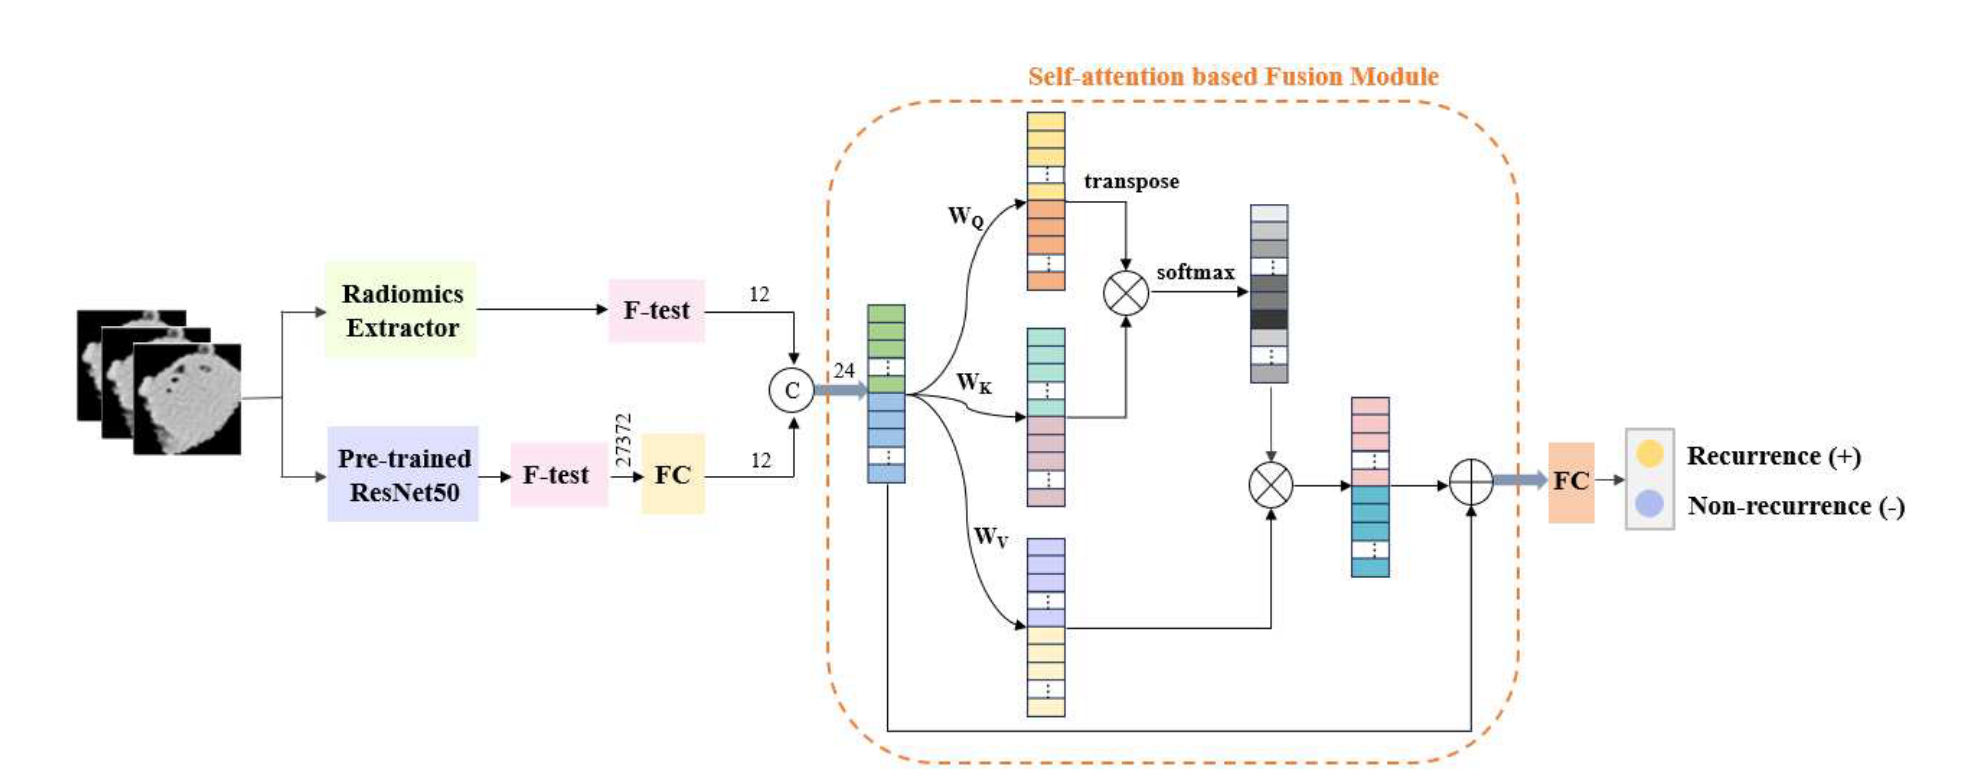
\includegraphics[width=1\textwidth]{figures/fig006.png}
    \caption*{Fonte: \cite{aiSelfAttentionBasedFusion2023}}
    \label{fig:fig006}
\end{figure}

% \newpage
\clearpage

%---------------------------------------------------------
\section{Objetivo}
\label{sec:cap1_objetivo}

Dado o contexto na qual o presente projeto de pesquisa está inserido, o objetivo deste será implementar e validar uma estratégia de fusão que combina características manuais extraídas da análise de textura radiômica e características profundas, para melhorar a expressividade e a habilidade de generalização do modelo de \gls{RNP}. Será utilizado imagens de \gls{RMC} e as doenças \gls{CMH} e \gls{CMD} como objetos de estudo para avaliar o desempenho da abordagem. Como objetivos específicos, têm-se:

\begin{enumerate}

\item Implementação do modelo, que utiliza características radiômicas e
características profundas.

\item Coleta de resultados em conjunto de dados públicos, como linha de base da análise.

\item Avaliação dos resultados iniciais.

\item Proposta de novas abordagens tanto no pré-processamento quanto na arquitetura, mediante coleta dos resultados.

\item Iteração e análise dos resultados obtidos, sua documentação e comparação.
\end{enumerate}

%---------------------------------------------------------
\section{Estrutura do trabalho}
\label{sec:cap1_estrutura_trabalho}

Esta proposta está organizada em seis capítulos, a saber:
O \textbf{Capítulo \ref{chap:intro}} apresenta a introdução, objetivo e contribuições desejadas. O \textbf{Capítulo \ref{chap:fundamentacao_teorica}} faz um aprofundamento teórico no tema de pesquisa estudando as técnicas consideradas primordiais deste trabalho e/ou que são utilizadas no desenvolvimento do experimento prático. No \textbf{Capítulo \ref{chap:trab_relacionados}} é estudado  os trabalhos recentes, não superior a cinco anos passados, de outros autores que estão de alguma forma relacionados com tema, sendo estes trabalhos relacionados oriundos de uma minuciosa revisão sistemática da literatura. No \textbf{Capítulo \ref{chap:metodologia}} é apresentada uma proposta de metodologia para a realização do experimento prático. O \textbf{Capítulo \ref{chap:proposta_experimental}} é uma proposta experimental que contempla os dados utilizados, informações do seu pré-processamento, hiperparâmetros planejados e demais informações assim como o cronograma do presente projeto de pesquisa. No \textbf{Capítulo \ref{chap:resultados_discussao}}, são apresentados os resultados parciais da prova de conceitos, considerando a arquitetura proposta no artigo que serviu como base. Finalmente, o \textbf{Capítulo \ref{chap:consideracoes_parciais}} apresenta consideração do presente projeto de pesquisa.

\chapter{FUNDAMENTAÇÃO TEÓRICA}
\label{chap:fundamentacao_teorica}

A proposta deste trabalho visa unificar informações das características radiômicas e características profundas oriundas de uma rede neural convolucional e, por conseguinte, propor uma arquitetura de autoatenção para identificar características discriminantes a fim de obter resultados relevantes na classificação de \gls{CAR}.

%--------------------------------------------------------
\section{Ressonância Magnética em Cardiomiopatia}
\label{sec:rmc}

A \gls{RMC} se tornou um dos principais métodos em imagem médica para avaliar a fisiologia e a função na doença cardíaca congênita. A \gls{RMC} possui funções que normalmente são obtidas por ecocardiografia, tendo como exemplo a velocidade média em um vaso, mas também apresenta características muito especiais como calcular a velocidade em um voxel de um milímetro em qualquer lugar no espaço tridimensional do vaso.
Usando a tecnologia atual de \gls{RMC}, os investigadores podem obter percepções únicas sobre a função ventricular, por exemplo, deformação ventricular regional \textit{in vivo}, movimento da parede e mecânica dos fluidos, por exemplo, visualização \textit{in vivo} de perfis de velocidade além de aumentar a precisão de medidas padrão aceitas pela fisiologia ou função ventricular, por exemplo, débito cardíaco, volumes ventriculares e massa. Devido ao rápido avanço da tecnologia, muitas técnicas de \gls{RMC} são experimentais ou ainda estão em fase de desenvolvimento clínico; no entanto, há muitas técnicas que são clinicamente úteis, por exemplo, medição do volume ventricular em pacientes com tamanho ventricular esquerdo limítrofe. Como muitas das técnicas experimentais atuais serão, sem dúvida, empregadas na prática clínica no futuro, os médicos devem estar cientes de todo o espectro de capacidades da \gls{RMC} \cite{fogelAssessmentCardiacFunction2000}.

Em muitos cenários clínicos, as limitações técnicas da ecocardiografia e a expressão fenotípica heterogênea tornaram tal avaliação difícil e a \gls{RMC} cardíaca emergiu como uma modalidade de imagem complementar útil para incorporar a ecocardiografia transtorácica de rotina. A \gls{RMC} cardíaca é única em sua alta resolução espacial e temporal com excelente contraste entre o \textit{pool} sanguíneo e o miocárdio, sem limitação de janela de imagem ou plano de imagem.
A heterogeneidade fenotípica da miocardiopatia hipertrófica é bem reconhecida pela dificuldade em sua identificação. Isto se complica ainda mais pois nem todos os pacientes com hipertrofia ventricular esquerda têm CMH, enquanto uma fisiopatologia semelhante à CMH com obstrução dinâmica do trato de saída do ventrículo esquerdo pode ser observada sem hipertrofia do ventrículo esquerdo, em um subgrupo de pacientes com anormalidades na válvula mitral e/ou no músculo papilar \cite{pontoneClinicalApplicationsCardiac2022}.

A CMH é uma doença heterogênea com expressão morfológica complexa que requer uma caracterização precisa da doença para um planejamento terapêutico ótimo e estratificação de risco. A \gls{RMC} cardíaca emergiu como um complemento útil para esses propósitos. Com a incorporação crescente de imagem multimodal na avaliação clínica da CMH, o entendimento sobre a importância de diferenças morfológicas sutis continuará a crescer, e pesquisas adicionais definirão novos marcadores prognósticos e melhorarão as estratégias de tratamentos atuais \cite{toCardiacMagneticResonance2011c}.

%Diferentemente de outras áreas que utilizam e geram majoritariamente dados textuais, a Medicina também faz uso massivo de imagens para composição de seus diagnósticos. Independentemente do propósito da imagem, nos últimos anos esses equipamentos também evoluíram e se tornaram mais precisos, proporcionando um volume maior de dados e imagens, que exigem uma maior capacidade de armazenamento (ISSA; BYERS; DAKSHANAMURTHY, 2014).

%Algumas modalidades médicas como a Ressonância Magnética Cardíaca (RMC) e a Tomografia Computadorizada (TC) são exemplos de exames que podem gerar objetos tridimensionais (3D) de estruturas específicas do corpo humano a partir de dezenas de fatias (BANKMAN; MORCOVESCU, 2002). Um outro aspecto que também desafia a comunidade médica é a fadiga visual, percebida quando o especialista realiza a análise contínua de muitas imagens.


% Expostos esses fatores, torna-se relevante o desenvolvimento de métodos inteligentes para armazenamento e recuperação dessas imagens médicas que são geradas diariamente. Nesse sentindo, os sistemas de Diagnóstico Auxiliado por Computador (Computer-Aided Diagnosis - CAD) têm o propósito de apoiar especialistas médicos em seus diagnósticos, uma vez que o tempo demandado para analisar essas imagens tem se tornado cada vez maior (DATTA et al., 2008).

%--------------------------------------------------------
\section{Análise Radiômica}
\label{sec:analise_radiomica}

A análise radiômica é um campo de pesquisa em rápida evolução, preocupada com a extração de informações quantitativas, incluindo padrões complexos que são difíceis de reconhecer ou quantificar pelo olho humano a cerca de imagens médicas, características estas chamadas de características radiômicas. As características radiômicas podem capturar características de tecidos e lesões, como forma e heterogeneidade, e podem, sozinhas ou em combinação com dados demográficos, histológicos, genômicos ou proteômicos, ser usadas para a resolução de problemas clínicos.

Mesmo que características radiômicas individuais podem se correlacionar com dados genômicos ou dados clínicos, o impacto da análise radiômica se torna mais relevante a medida que mais informações são por ela extraídas. Tipicamente centenas de características, uma fração do total que é extraído, contribuem para identificação de uma doença específica e é processada usando técnicas de aprendizado de máquina. As características radiômicas podem ser subdivididas em estatísticas, incluindo as baseadas em histograma e textura; modelo; transformação; e forma. A extração pode ser dada em regiões de interesse de 2-dimensões (2D) e 3-dimensões (3D)  \cite{mayerhoeferIntroductionRadiomics2020}.


%--------------------------------------------------------
\subsection{Características por Histograma}

Os descritores estatísticos mais simples são baseados no histograma global de níveis de cinza e incluem média de nível de cinza, máximo, mínimo, variância e percentis. Como essas características são baseadas em análises de \textit{pixel} único ou \textit{voxel} único (3D), elas são chamadas de características de primeira ordem. Algumas características mais sofisticadas incluem assimetria e curtose que descrevem a forma da distribuição da intensidade dos dados: a assimetria reflete a assimetria da curva da distribuição de dados para a esquerda (assimetria negativa, abaixo da média) ou direita (assimetria positiva, acima da média), enquanto a curtose reflete a caudalidade de uma distribuição de dados em relação a uma distribuição gaussiana devido a \textit{outliers}. Outras características incluem histograma entrópico e uniformidade, e também é comumente chamado de energia.

%--------------------------------------------------------
\subsection{Características de Textura}

Uma abordagem simples para a descrição de textura radiômica é a análise do gradiente absoluto, que reflete o grau ou a abruptidade das flutuações de intensidade de nível de cinza em uma imagem. Para dois \textit{pixels} ou \textit{voxels} adjacentes, o gradiente é o máximo possível quando um for preto e o outro branco, enquanto se ambos os \textit{pixels} forem pretos (ou ambos forem brancos) o gradiente nessa localidade é zero. Similares aos histogramas, as características por gradiente incluem média, variância, assimetria e curtose.

A Figura \ref{fig:fig001} Imagens de \gls{TC} e \gls{PET} com contraste de um câncer de pulmão parcialmente necrótico no lobo inferior esquerdo. Os mapas de características radiômicas são gerados ao mover uma pequena janela retangular sobre a imagem de \glas{TC}, calculando o valor da característica em cada posição. Esses mapas refletem diferentes aspectos da heterogeneidade do metabolismo da glicose no tumor. Cada mapa representa uma única característica radiômica, onde valores altos indicam intensidades elevadas no mapa de níveis de cinza.


\captionsetup{justification=centering}
\begin{figure}[htbp]
    \centering
    \caption{Exemplos de aplicação da análise radiômica na identificação de tumores. 
    \newline CE = \textit{Contrast Enchanced}, HH = \textit{high-high} (filtro passa-alta)}
    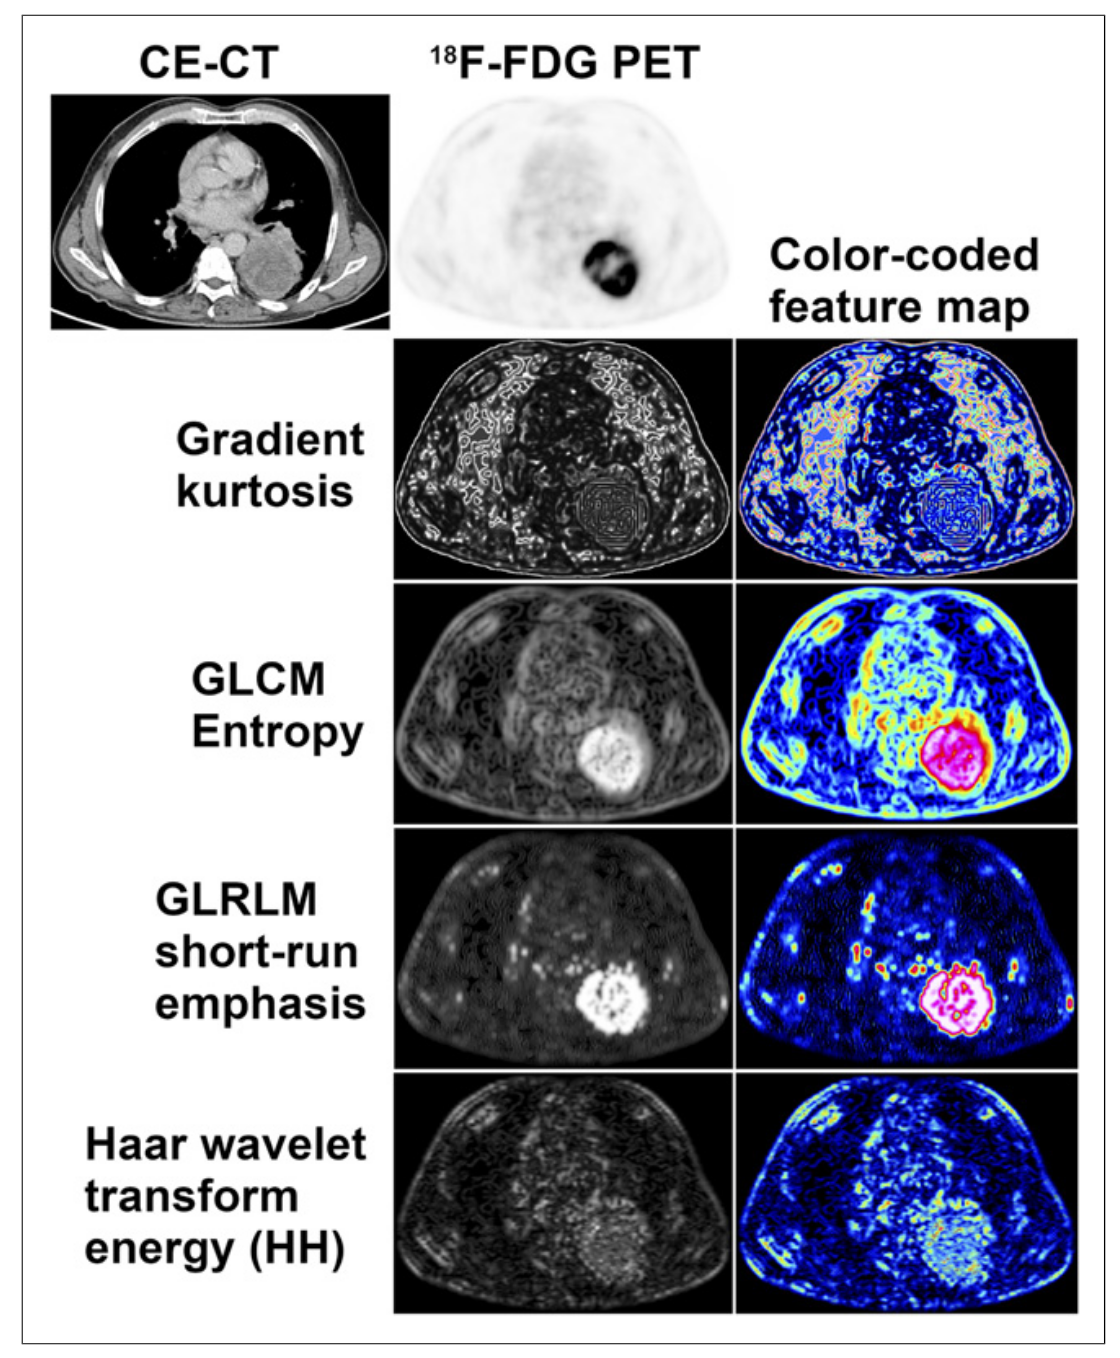
\includegraphics[width=0.6\textwidth]{figures/fig001.png}
    \caption*{Autor: \cite{mayerhoeferIntroductionRadiomics2020}}
    \label{fig:fig001}
\end{figure}

 A matriz de coocorrência de níveis de cinza, do termo \gls{GLCM}, é um histograma em níveis de cinza de segunda ordem. O GLCM captura relações espaciais entre pares de \textit{pixels} ou \textit{voxels} com níveis de níveis de cinza pré-definidos, em diferentes direções (horizontal, vertical ou diagonal para análise 2D, 13 direções para 3D) e com uma distância pré-definida entre os \textit{pixels} ou \textit{voxels}. As características de GLCM incluem entropia, uma medida composta pela medida da inomogeneidade ou aleatoriedade dos níveis de cinza, momento angular de segunda ordem (também chamado de uniformidade ou energia), que reflete a homogeneidade ou ordem dos níveis de cinza e contraste, que enfatiza as diferenças nos níveis de cinza entre \textit{pixels} ou \textit{voxels} pertencentes a um par de \textit{pixel} ou \textit{voxel}. A Figura \ref{fig:fig002} ilustra um matriz que atua como um contador dos pares de \textit{pixel} ou \textit{voxel}.

 A matriz de comprimento de corrida de níveis de cinza, do termo 
 \textit{Gray-Level Run-length Matrix} (GLRLM), fornece informações sobre a distribuição espacial das sequências de \textit{pixels} consecutivos com os mesmos níveis de cinza, em uma ou mais direções, em 2 ou 3 dimensões. As características da GLRLM incluem fração, que avalia a porcentagem de \textit{pixels} ou \textit{voxels} dentro da região de interesse que fazem parte das sequências e, portanto, reflete a granulosidade. 

A matriz de zona do tamanho dos níveis de cinza, do termo \textit{Gray-Level Size Zone Matrix} (GLSZM), é baseada no mesmo princípio do GLRLM porém aqui, contagens do número de grupos (chamados zonas) de \textit{pixels} ou \textit{voxels} vizinhos interconectados com o mesmo nível de cinza formam a base para a matriz, como visto na Figura \ref{fig:fig002}. Uma textura mais homogênea resultará em uma matriz mais ampla e plana. A GLSZM não é calculada para diferentes direções, mas pode ser calculada para diferentes distâncias de \textit{pixels} ou \textit{voxels} que definem a vizinhança. As características da GLSZM podem ser calculadas em 2 dimensões (8 \textit{pixels} vizinhos) ou 3 dimensões (26 \textit{voxels} vizinhos) e, seguindo as definições da GLRLM, incluem fração (porcentagem de \textit{pixels} ou \textit{voxels} que fazem parte das zonas), ênfase em zonas pequenas e grandes, entre outras.

\begin{figure}[htbp]
    \centering
    \caption{Aplicação de Vizinhos em Abordagens Radiômicas}
    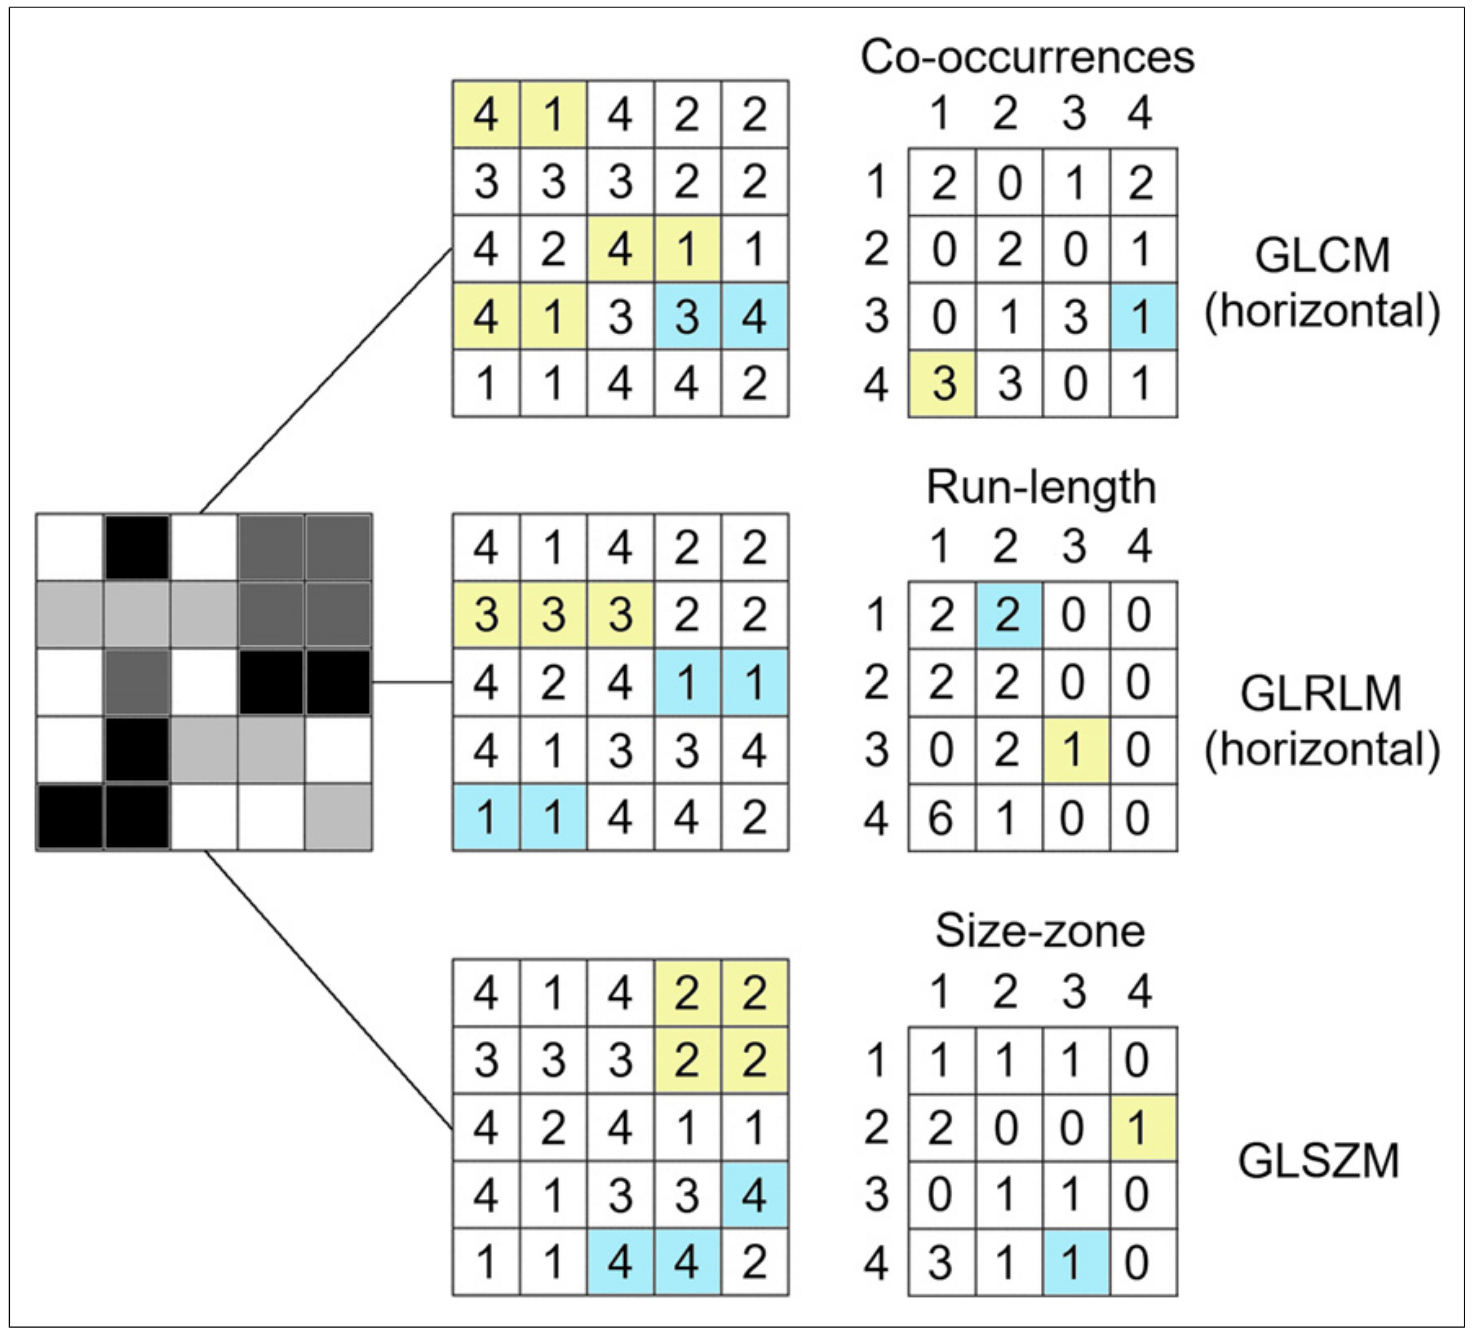
\includegraphics[width=0.6\textwidth]{figures/fig002.png}
    \caption*{Autor: \cite{mayerhoeferIntroductionRadiomics2020}}
    \label{fig:fig002}
\end{figure}

%--------------------------------------------------------
\subsection{Características de Modelo}

As análises baseadas em modelos visam interpretar características em níveis de cinza espaciais para caracterizar objetos ou formas. Um modelo parametrizado de geração de textura é calculado e ajustado à região de interesse, do termo \gls{ROI}, e seus parâmetros estimados são utilizados como características radiômicas. O modelo autorregressivo é um exemplo de abordagem baseada em modelo e baseia-se na ideia de que o nível de cinza de um \textit{pixel} é uma soma ponderada dos níveis de cinza de 4 \textit{pixels} vizinhos. Além disso, o $\sigma$, o qual carrega informações sobre a variância do erro de previsão mínimo, mede a regularidade da textura. A análise fractal também produz recursos que podem ser usados na análise radiômica, em particular a dimensão fractal, que reflete a taxa de adição de detalhe estrutural com o aumento da magnificação, escala ou resolução e, portanto, serve como uma medida de complexidade. A lacunaridade, um recurso que mede a falta de invariância rotacional ou translacional, reflete a inomogeneidade \cite{mayerhoeferIntroductionRadiomics2020}.

%--------------------------------------------------------
\subsection{Características de Transformação}
Métodos baseados em transformadas, incluindo transformadas de \textit{Fourier}, \textit{Gabor} e de \textit{wavelets} de \textit{Haar}, analisam padrões de níveis de cinza em um espaço diferente. A transformada discreta \textit{wavelet} de \textit{Haar}, por exemplo, analisa o conteúdo da frequência de uma imagem em diferentes escalas. A decomposição por \textit{wavelets} de uma imagem é possível aplicando um par de filtros espelhados em quadratura, um filtro de passa-alta e um de passa-baixa. Embora o filtro de passa-alta destaque as mudanças no nível de cinza e, assim, enfatize detalhes da imagem, o filtro de passa-baixa suaviza a imagem em termos de nível de cinza, removendo detalhes da imagem. Após a decomposição do sinal, um conjunto de canais de frequência orientados espacialmente está disponível, o qual é usado para descrever a variabilidade local da imagem. As energias dentro dos canais de frequência são então usadas como características. A filtragem de passa-alta em ambas as direções, parte inferior da Figura \ref{fig:fig001}, captura detalhes diagonais, a filtragem de passa-alta seguida por filtragem de passa-baixa captura bordas verticais, a filtragem de passa-baixa seguida da filtragem de passa-alta captura bordas horizontais, e a filtragem de passa-baixa em ambas as direções captura as frequências mais baixas, em diferentes escalas. Notavelmente, a transformação por \textit{wavelets} pode ser usada não apenas para a geração de características radiômicas, mas também para segmentação de imagens ou como um passo de pré-processamento para análise de textura \cite{mayerhoeferIntroductionRadiomics2020}.

%---------------------------------------------------------
\section{Redes Neurais Convolucionais}
\label{sec:cnn}


Os autores \citeonline{lecunHandwrittenDigitRecognition1989} pesquisaram sobre o reconhecimento de caracteres em documentos escritos à mão, criando a arquitetura LeNet, uma rede que consiste em camadas convolucionais seguidas por camadas de \textit{pooling}, e finalizando com camadas totalmente conectadas. Os autores introduziram o \textit{backpropagation} a redes convolucionais, permitindo o aprendizado automático e substituindo o uso de técnicas para escolha manual de coeficientes. \citeonline{lecunHandwrittenDigitRecognition1989}, ainda estudando a classificação de caracteres, expandem a LeNet para a LeNet-5, uma rede que firmou a superioridade das redes convolucionais na tarefa de classificação de imagens se comparado a outros métodos da época.

Como o nome sugere, a camada convolucional desempenha um papel vital no funcionamento da \gls{CNN}. Os parâmetros das camadas concentram-se no uso de \textit{kernels} treináveis. Esses \textit{kernels} geralmente são pequenos em dimensionalidade espacial, mas se estendem por toda a profundidade da entrada. Quando os dados passam por uma camada convolucional, ela aplica cada filtro na dimensionalidade espacial da entrada para produzir um mapa de ativação 2D. À medida que se percorre a entrada, o produto escalar é calculado para cada valor nesse \textit{kernel}. A partir disso, a rede aprenderá \textit{kernels} que ``disparam'' quando detectam uma característica específica em uma determinada posição espacial da entrada. Esses são comumente conhecidos como ativações conforme descrito na Figura \ref{fig:fig024}.

\begin{figure}[h!]
    \centering
    \caption{Representação visual da camada convolucional. O elemento central do \textit{kernel} é aplica no vetor de entrada, que é calculado e substituído pela ponderada dele mesmo e de quaisquer pixels próximos.}
    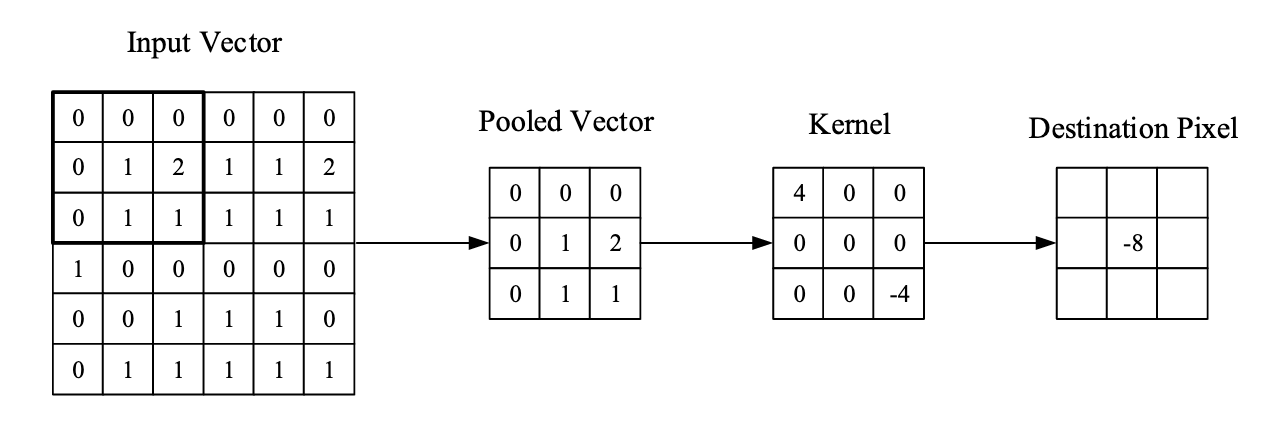
\includegraphics[width=0.6\textwidth]{figures/fig024.png}
    \caption*{Fonte: \cite{osheaIntroductionConvolutionalNeural2015c}}
    \label{fig:fig024}
\end{figure}

Cada \textit{kernel} terá um mapa de ativação correspondente, que será empilhado ao longo da dimensão de profundidade para formar o volume completo de saída da camada convolucional. Como mencionado anteriormente, treinar redes neurais artificiais tendo imagens como entrada resulta em modelos demasiadamente grandes para serem treinados de forma eficaz. Isso ocorre devido à conexão totalmente densa dos neurônios padrão das redes neurais artificiais. Para mitigar esse problema, cada neurônio em uma camada convolucional é conectado apenas a uma pequena região do volume de entrada \cite{osheaIntroductionConvolutionalNeural2015c}. 

A dimensionalidade dessa região é comumente chamada de ``tamanho do campo receptivo'' do neurônio. A magnitude da conectividade ao longo da profundidade geralmente é igual à profundidade da entrada. Por exemplo, se o entrada para a rede for uma imagem de tamanho 64x64x3 (uma imagem colorida RGB com dimensionalidade de 64x64) e definirmos o tamanho do campo receptivo como 6x6, teríamos um total de 108 pesos em cada neurônio dentro da camada convolucional (6x6x3, onde 3 é a magnitude da conectividade na profundidade do volume). Para colocar isso em perspectiva, um neurônio padrão visto em outras formas de redes neurais artificiais conteria $12.288$ pesos cada. 

Camadas convolucionais também conseguem reduzir significativamente a complexidade do modelo através da otimização de sua saída. Essas otimizações são feitas por meio de três hiperparâmetros: profundidade, \textit{stride} e \textit{zero-padding}. 

A profundidade do volume de saída produzido pelas camadas convolucionais pode ser definida manualmente através do número de neurônios dentro da camada para uma mesma região da entrada. Isso pode ser observado em outras formas de redes neurais artificiais, onde todos os neurônios da camada oculta estão diretamente conectados a cada neurônio anterior. Reduzir esse hiperparâmetro pode minimizar significativamente o número total de neurônios da rede, mas também pode reduzir as capacidades de reconhecimento de padrões do modelo. 

Também é possível definir o \textit{stride}, que determina como é configurada a profundidade em torno da dimensionalidade espacial da entrada para posicionar o campo receptivo. Por exemplo, se o \textit{stride} for definido como 1, obtém-se um campo receptivo fortemente sobreposto, produzindo ativações extremamente grandes. Por outro lado, ao configurar o \textit{stride} para um número maior reduz a sobreposição e gera uma saída com dimensões espaciais menores.  

O \textit{zero-padding} é o processo de adicionar bordas à entrada, sendo um método eficaz para proporcionar maior controle sobre a dimensionalidade dos volumes de saída. É importante entender que, ao se usar dessas técnicas, a dimensionalidade espacial da saída das camadas convolucionais é alterada. Para este cálculo pode-se usar a seguinte Equação \ref{eq:cnn_output}.

\begin{equation}
\frac{(V - R) + 2Z}{S + 1}
\label{eq:cnn_output}
\end{equation}

O termo $V$ representa o tamanho do volume de entrada (altura x largura x profundidade), $R$ representa o tamanho do campo receptivo, $Z$ é a quantidade de \textit{zero-padding} definida e $S$ refere-se ao \textit{stride}. Se o resultado calculado a partir desta equação não for um número inteiro, o \textit{stride} foi configurado incorretamente, pois os neurônios não conseguirão se ajustar perfeitamente à entrada \cite{osheaIntroductionConvolutionalNeural2015c}.

%---------------------------------------------------------
\section{ResNet}
\label{sec:resnet}

A \textit{ResNet} (Rede Residual) é uma arquitetura de rede neural profunda amplamente utilizada em tarefas de visão computacional, como classificação de imagens, detecção de objetos e segmentação de imagens. Ela foi introduzida por \citeonline{heDeepResidualLearning2015}, e se destacou por ganhar a competição \textit{ImageNet} em 2015 com uma precisão significativamente maior do que as arquiteturas anteriores. A principal característica da \textit{ResNet} é sua capacidade de treinar redes muito profundas sem sofrer com o problema do ``desvanecimento do gradiente'' que afeta principalmente redes neurais profundas e impede o treinamento de progredir por conta de valores muito baixos de gradiente, problema este muito comum em redes tradicionais muito profundas. A \textit{ResNet} introduz um conceito chave chamado bloco residual que é um componente da rede onde a entrada do bloco é somada à sua saída antes de passar para a próxima camada. Esta conexão direta é chamada de conexão de salto e pode ser observada na Figura \ref{fig:fig013}.

\begin{figure}[h!]
    \centering
    \caption{Conexão de Salto}
    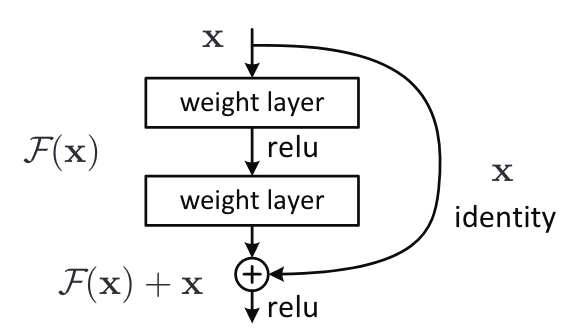
\includegraphics[width=0.6\textwidth]{figures/fig013.png}
    \caption*{Fonte: \cite{aiSelfAttentionBasedFusion2023}}
    \label{fig:fig013}
\end{figure}

A ResNet é composta por vários blocos residuais empilhados.
Existem várias versões da \textit{ResNet}, como \textit{ResNet}-18, \textit{ResNet}-34, \textit{ResNet}-50, \textit{ResNet}-101, e \textit{ResNet}-152, onde os números indicam a profundidade total da rede, ou seja, o número de camadas.

%--------------------------------------------------------
\subsection{Extração de Características Profundas}
\label{subsec:extract_features}

Para extrair características profundas das imagens de \gls{RMC}, foi empregada a arquitetura pré-treinada de uma rede \textit{ResNet50}. As redes \textit{ResNet50} ficaram muito conhecidas em meados do ano de 2015 por vencer diversas competições em visão computacional, includindo 1º lugar na competição de classificação de imagens \textit{ILSVRC} 2015. As redes \textit{ResNet}, do termo \textit{Residual Networks}, inovaram em sua época trazendo uma nova forma de treinar modelos que possuem maior profundidade, chegando a mais de 100 camadas, com resultados superiores à outros modelos convolucionais competitivos, como o \textit{VGG19}, sem sofrer sintomas comuns a redes neurais muito profundas como o \textit{overfitting} e a saturação ou a ausência dos gradientes em tempo de treino. Os autores da \textit{ResNet} sugeriram o uso de saltos de conexão entre as camadas da rede afim de manter os gradientes relevantes e controlados entre uma camada e outra.  A \textit{ResNet50} é um modelo de rede neural convolucional profunda de $50$ camadas que compreende muitos blocos residuais. A cada bloco, se encontram módulos de convolução e uma conexão de salto que transfere a informação do bloco anterior para o próximo bloco. A conexão de salto ajuda a reter a informação semântica mais baixa aprendida nas camadas anteriores, que de outra forma se tornaria abstrata devido à conexão de longa cadeia. A conexão de salto também evita que o gradiente desapareça nas camadas mais profundas, fornecendo um caminho alternativo para a retropropagação. A informação da conexão de salto é adicionada à informação calculada em cada bloco \cite{heDeepResidualLearning2015}.

Várias abordagens de sucesso aplicaram redes convolucionais para extrair características genéricas para tarefas de recuperação de imagens e obtiveram resultados promissores. Elas utilizam principalmente o poder das características locais para gerar uma representação de uma imagem genérica baseada em redes convolucionais pré-treinadas. As representações das camadas finais da rede convolucional são utilizadas para capturar características semânticas para o fim de nível de categoria à classificação que o modelo se dispõe \cite{alzubiContentbasedImageRetrieval2017b}.

%---------------------------------------------------------
\section{Rede Squeeze and Excitation}
\label{sec:se_net}

Para cada camada convolucional, um conjunto de filtros é aprendido para expressar padrões de conectividade espacial local ao longo dos canais de entrada. Em outras palavras, espera-se que os filtros convolucionais sejam combinações informativas ao fundir informações espaciais e baseadas nos canais dentro de campos receptivos locais.
Ao empilhar uma série de camadas convolucionais intercaladas com não linearidades e redução de amostragem, as \gls{CNN}s são capazes de capturar padrões hierárquicos com campos receptivos globais, funcionando como descrições de imagem poderosas \cite{huSqueezeandExcitationNetworks2018}. 

Estudos de \citeonline{huSqueezeandExcitationNetworks2018}, demonstraram que o desempenho das redes pode ser aprimorado ao incorporar explicitamente mecanismos de aprendizado que ajudam a capturar correlações espaciais, sem a necessidade de supervisão adicional. Neste sentido, foi proposto um mecanismo que permite à rede realizar a recalibração de características, através do qual ela pode aprender a usar informações globais para enfatizar seletivamente características informativas e suprimir aquelas menos úteis. Este estudo intitulado \gls{SE} Net, investiga um aspecto diferente no design arquitetural, a relação entre canais ao introduzir o bloco \gls{SE}.

Os blocos \gls{SE} podem ser construídos para qualquer transformação conforme a indica a Equação \ref{eq:se_transform}. 

\begin{equation}
\mathcal{F}_{tr} : \mathbf{X} \rightarrow \mathbf{U}, \mathbf{X} \in \mathbb{R}^{H' \times W' \times C'}, \mathbf{U} \in \mathbb{R}^{H \times W \times C}
\label{eq:se_transform}
\end{equation}

Sendo $\mathbf{V} = [\mathbf{v}_1, \mathbf{v}_2, \ldots, \mathbf{v}_C]$ os filtros de aprendidos onde $\mathbf{v}_C$ se refere aos parâmetro de $c$-ésimo filtro. As saídas das convoluções podem ser escritas da seguinte forma: $\mathcal{F}_{tr} \mathbf{U} = [\mathbf{u}_1, \mathbf{u}_2, \ldots, \mathbf{u}_C]$, sendo o termo $\mathbf{u}_C$ descrito na equação \ref{eq:se}. 

\begin{equation}
\mathbf{u}_c = \mathbf{v}_c \ast \mathbf{X} = \sum_{s=1}^{C'} \mathbf{v}_c^s \ast \mathbf{x}^s
\label{eq:se}
\end{equation}

O termo $\ast$ denota convolução, $\mathbf{v}_c$ é um filtro espacial 2D e representa um único canal de $\mathbf{v}_c$ que atua no canal correspondente de $\mathbf{X}$. 
Tendo como o objeto garantir que a rede seja capaz de aumentar sua sensibilidade a características informativas, para que possam ser exploradas por transformações subsequentes, e suprimir as menos úteis. Foi proposto um modelo explícito das interdependências de canal para recalibrar as respostas dos filtros em duas etapas — \textit{squeeze} e \textit{excitation} —, antes de serem alimentadas na transformação subsequente. Um diagrama de um bloco de construção \gls{SE} é demonstrado na Figura \ref{fig:fig025}.

\begin{figure}[h!]
    \caption{Fluxo do Bloco SE - Após blocos convolucionais normais, uma cama da de \textit{squeeze} seguida e uma camada de \textit{excitation} é aplicada e por fim os valores originais são escalonados pelo resultado.}
    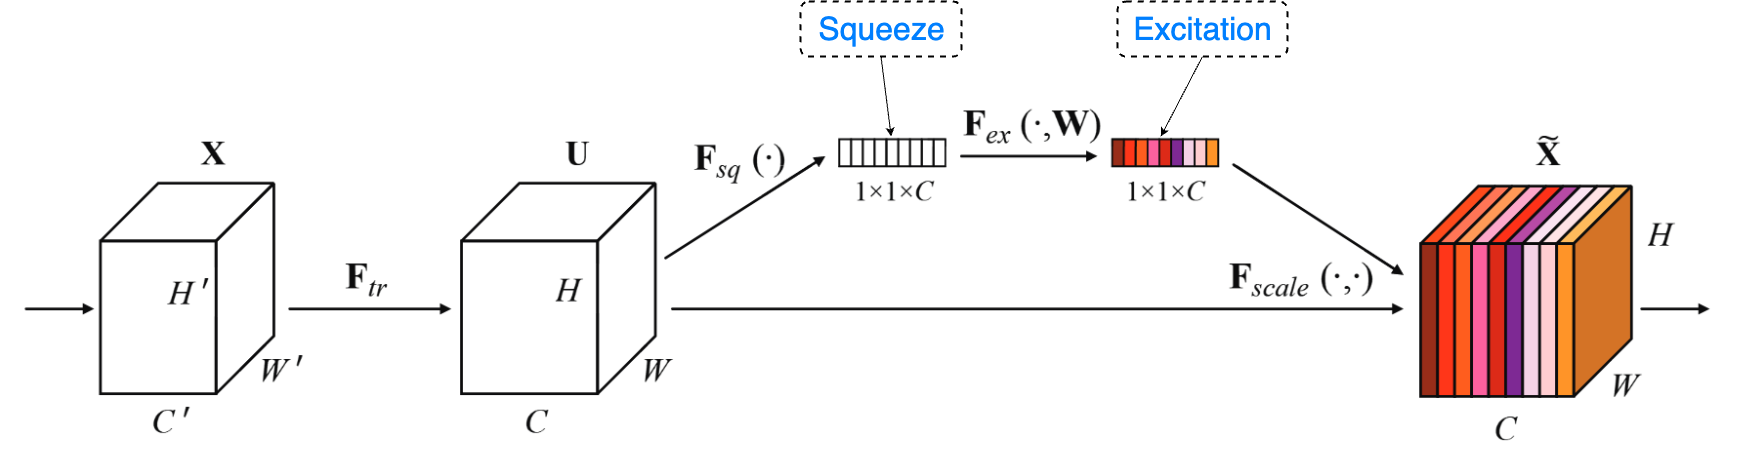
\includegraphics[height=0.27\textwidth]{figures/fig025.png}
    \caption*{Fonte: Adaptado de \cite{huSqueezeandExcitationNetworks2018}}
    \label{fig:fig025}
\end{figure}


%---------------------------------------------------------
\subsection{Squeeze: Informação Global}
\label{subsec:squeeze}

Para lidar com o problema de explorar as dependências entre os canais, é considerado o primeiro sinal de cada canal nas características de saída. Cada um dos filtros aprendidos opera com um campo receptivo local e, consequentemente, cada unidade da saída da transformação $\mathbf{U}$ é incapaz de explorar informações contextuais fora dessa região. Esse problema se torna ainda mais grave nas camadas mais baixas da rede, cujos campos receptivos são menores.

Para mitigar esse problema, foi proposto comprimir as informações espaciais globais em um descritor de canal. Isso é obtido por meio de uma instrução de \textit{average pooling} global para gerar estatísticas específicas de cada canal. O cálculo do \textit{average pooling} pode ser conferido na Equação \ref{eq:avgpool}.

\begin{equation}
z_c = \mathbf{F}_{sq}(\mathbf{u}_c) = \frac{1}{H \times W} \sum_{i=1}^{H} \sum_{j=1}^{W} u_c(i, j)
\label{eq:avgpool}
\end{equation}

%---------------------------------------------------------
\subsection{Excitation: Recalibração Adaptativa}
\label{subsec:excitation}

Para aproveitar as informações agregadas na operação de \textit{squeeze}, uma segunda operação que tem como objetivo capturar completamente as dependências entre os canais. Para cumprir esse objetivo, a função deve atender a dois critérios: primeiro, ela precisa ser flexível (em particular, deve ser capaz de aprender uma interação não linear entre os canais) e, segundo, ela deve aprender uma relação não mutuamente exclusiva, pois é de interesse garantir que vários canais possam ser enfatizados, em vez de apenas uma ativação \textit{one-hot}. Para atender a esses critérios, emprega-se um mecanismo de \textit{gating} simples com uma ativação sigmoide conforme demonstrado na Equação \ref{eq:excitation}:

\begin{equation}
\mathbf{s} = \mathbf{F}_{ex}(\mathbf{z}, \mathbf{W}) = \sigma(g(\mathbf{z}, \mathbf{W})) = \sigma(\mathbf{W}_2 \delta(\mathbf{W}_1 \mathbf{z}))
\label{eq:excitation}
\end{equation}

\noindent sendo o que o termo $\delta$ se refere à função de ativação ReLU \cite{nairRectifiedLinearUnits}, $W_1 \in \mathbb{R}^{\frac{C}{r} \times C}$ e $W_2 \in \mathbb{R}^{C \times \frac{C}{r}}$. Para limitar a complexidade do modelo e auxiliar na generalização, o mecanismo de \textit{gating} é parametrizado formando um gargalo com duas camadas totalmente conectadas ao redor da não linearidade, ou seja, uma camada de redução de dimensionalidade com os parâmetros $W_1$ e razão de redução $r$, seguida de uma ReLU e, em seguida, uma camada de aumento de dimensionalidade com os parâmetros $W_2$. A saída final do bloco é obtida ao redimensionar a saída da transformação $U$ com as ativações conforme Equação \ref{eq:se_scale}.

\begin{equation}
\tilde{\mathbf{x}}_c = \mathbf{F}_{scale}(\mathbf{u}_c, s_c) = s_c \cdot \mathbf{u}_c 
\label{eq:se_scale}
\end{equation}

\noindent onde $\tilde{\mathbf{X}} = [\tilde{\mathbf{x}}_1, \tilde{\mathbf{x}}_2, \dots, \tilde{\mathbf{x}}_C]$ e $\mathbf{F}_{scale}(\mathbf{u}_c, s_c)$ se referem a multiplicação no nível dos canais entre os mapas de características $\mathbf{u}_c \in \mathbb{R}^{H \times W}$ e o valor escalar $s_c$.

%---------------------------------------------------------
\subsection{Utilização em redes conhecidas: SE-Resnet}
\label{subsec:util_resnet}

A flexibilidade do bloco \gls{SE} significa que ele pode ser aplicado diretamente a transformações além das convoluções padrão. Para ilustrar esse ponto, os autores desenvolveram as redes \gls{SE}  integrando blocos \gls{SE} em arquiteturas modernas com \textit{designs} sofisticados. A Figura \ref{fig:fig026} demonstra o esquema de um módulo SE-ResNet. Nele, a transformação do bloco \gls{SE}, $F_{tr}$, é considerada o ramo não identidade de um módulo residual. As operações de \textit{squeeze} e \textit{excitation} atuam antes da soma com o ramo identidade.


\begin{figure}[h!]
    \centering
    \caption{Módulo SE-Resnet}
    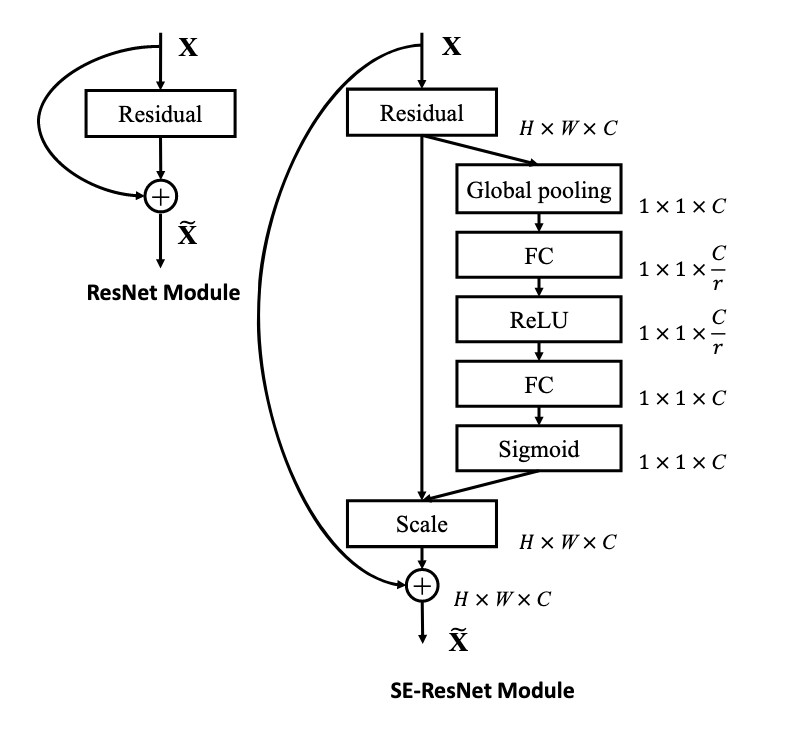
\includegraphics[width=0.6\textwidth]{figures/fig026.png}
    \caption*{Fonte: Adaptado de \cite{huSqueezeandExcitationNetworks2018}}
    \label{fig:fig026}
\end{figure}

Para que o bloco SE proposto seja viável na prática, ele deve fornecer um equilíbrio eficaz entre a complexidade do modelo e o desempenho, o que é importante para escalabilidade. Foi definido uma razão de redução $r$ como 16 em todos os experimentos, exceto onde indicado de outra forma. 

O valor $r$ é um hiperparâmetro importante pois permite variar a capacidade e o custo computacional dos blocos \gls{SE} no modelo. O autor do trabalho conduz experimentos baseados no SE-ResNet-50 para uma variedade de valores diferentes de $r$. A comparação vista na Figura  \ref{fig:fig027}, revela que o desempenho não melhora monotonicamente com o aumento da capacidade. Isso provavelmente é resultado do bloco SE ajustar em excesso as interdependências de canal do conjunto de treinamento. Definir $r = 16$ alcançou um bom equilíbrio entre precisão e complexidade e, consequentemente, foi o valor utilizado pelos autores nos experimentos. O Algoritmo \ref{alg:se_block} reflete a implementação do bloco \gls{SE}.

\begin{figure}[h!]
    \centering
    \caption{Conjunto de Validação Aplicado na SE-ResNet-50}
    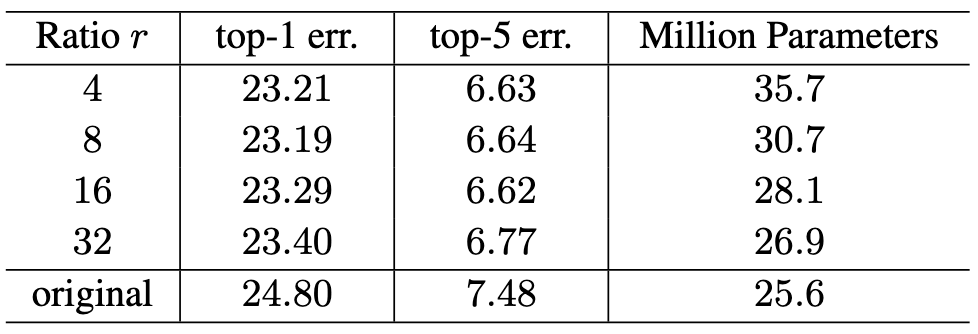
\includegraphics[width=0.6\textwidth]{figures/fig027.png}
    \caption*{Fonte: Adaptado de \cite{huSqueezeandExcitationNetworks2018}}
    \label{fig:fig027}
\end{figure}

% ----------------- ALGORITMO SQUEEZE AND EXCITATION NET ------------------
\begin{algorithm}
\caption{Bloco Squeeze-and-Excitation (SE)}
\label{alg:se_block}
\textbf{Entrada:} Mapa de características $\mathbf{U} \in \mathbb{R}^{H \times W \times C}$\\
\textbf{Saída:} Mapa de características recalibrado $\tilde{\mathbf{U}} \in \mathbb{R}^{H \times W \times C}$
\begin{algorithmic}[1]
\STATE \textbf{Squeeze:} Executa o \textit{average pooling} global para agregar as dimensões espaciais:
\[
z_c = \frac{1}{H \times W} \sum_{i=1}^H \sum_{j=1}^W u_c(i, j), \quad \forall c \in \{1, \dots, C\}
\]
\STATE \textbf{Excitation:} Usa duas camadas totalmente conectadas para modelar a interdependência dos canais:
\[
\mathbf{s} = \sigma(\mathbf{W}_2 \delta(\mathbf{W}_1 \mathbf{z}))
\]
onde:
\begin{itemize}
    \item $\mathbf{W}_1 \in \mathbb{R}^{\frac{C}{r} \times C}$: Camada de redução de dimensionalidade
    \item $\mathbf{W}_2 \in \mathbb{R}^{C \times \frac{C}{r}}$: Camada de restauração da dimensão original
    \item $\delta$: Ativação ReLU
    \item $\sigma$: Ativação Sigmoide
\end{itemize}
\STATE \textbf{Rescala:} Recalibra o mapa de características usando as ativações:
\[
\tilde{\mathbf{u}}_c = s_c \cdot \mathbf{u}_c, \quad \forall c \in \{1, \dots, C\}
\]
\RETURN $\tilde{\mathbf{U}} = [\tilde{\mathbf{u}}_1, \tilde{\mathbf{u}}_2, \dots, \tilde{\mathbf{u}}_C]$
\end{algorithmic}
% \caption*{Fonte: Autor}
\end{algorithm}


%--------------------------------------------------------
\section{Arquitetura Transformers}
\label{sec:transformers}

O \textit{transformers} é uma arquitetura que possui como um de seus propósitos resolver as limitações das arquiteturas recorrentes e sua dificuldade em manter as relações entre pontos dentre as camadas recorrentes além das restrições vinculadas ao custo de computação sequencial. O modelo de arquitetura \textit{transformers} se utiliza do mecanismo de atenção e este se tornou parte integral dos modelos de modelagem de sequências e transdução convincentes em várias tarefas, permitindo a modelagem de dependências sem considerar a distância entre elas nas sequências de entrada ou saída. Os \textit{transformers} como arquitetura descarta o uso de módulos de recorrência e se utiliza inteiramente do mecanismo de atenção para capturar as dependências globais entre entrada e saída. Os \textit{transformers} também são responsáveis por um ganho significante em paralelismo em sua execução \cite{vaswaniAttentionAllYou2023}.

\begin{figure}[htbp]
    \centering
    \caption{Arquitetura \textit{Transformers}}
    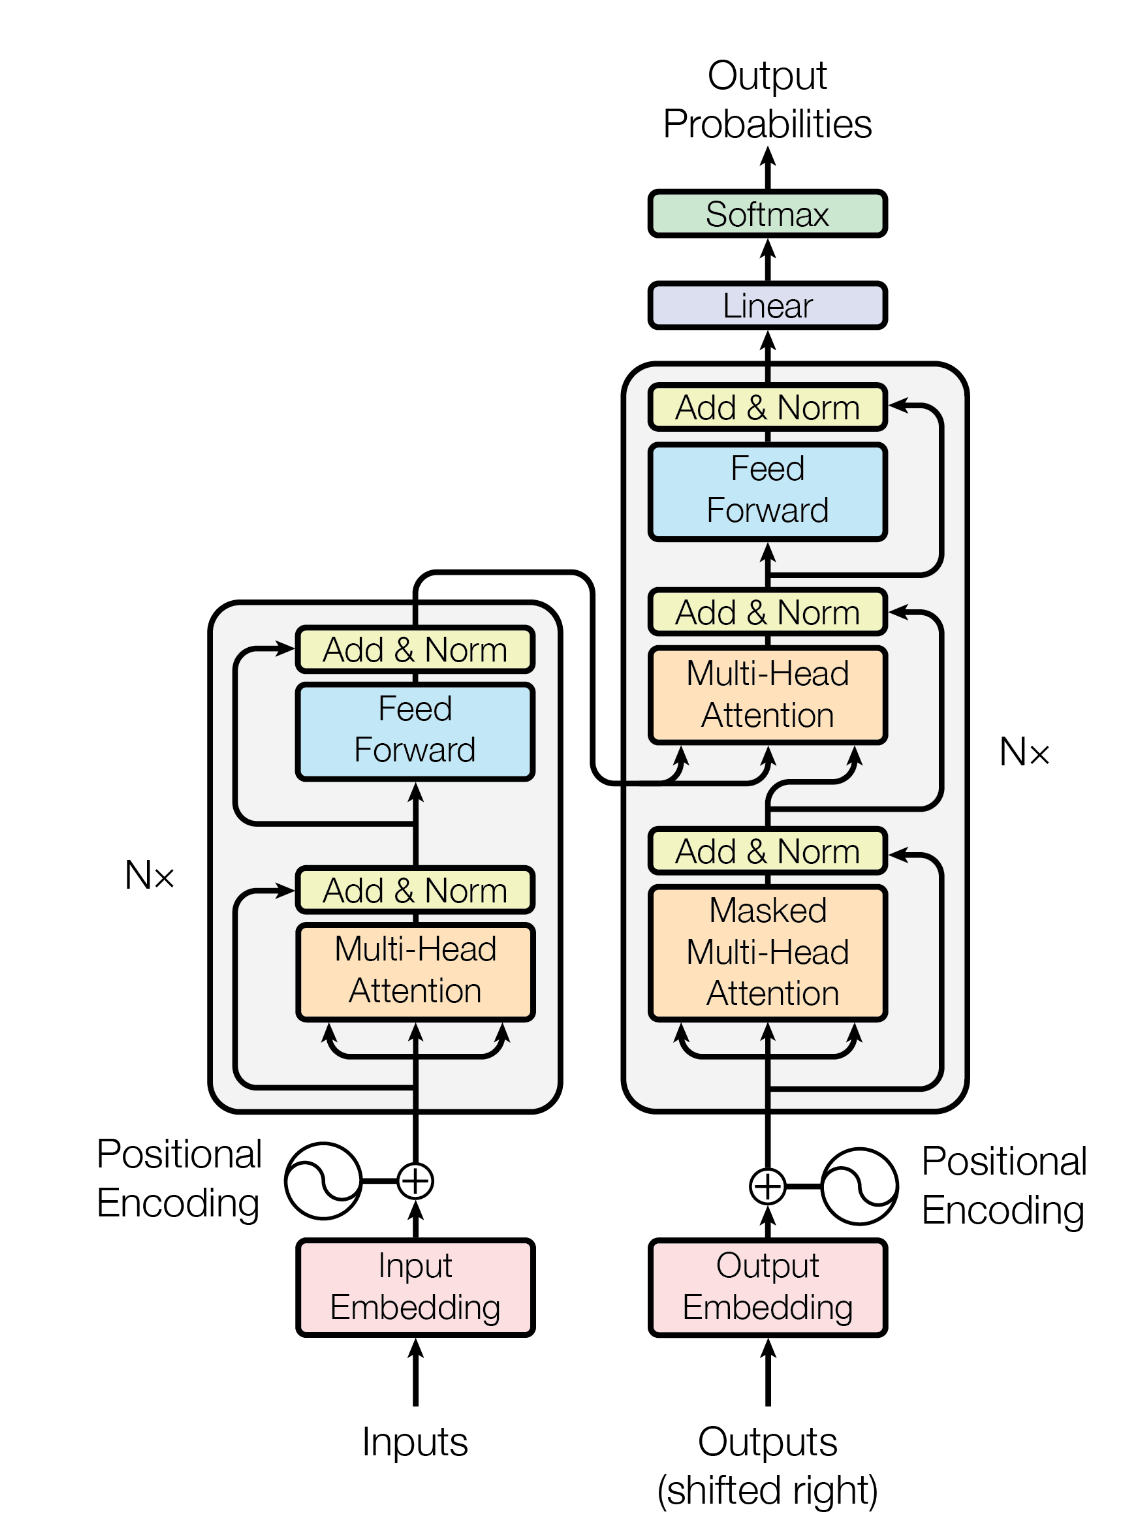
\includegraphics[scale=0.6]{figures/fig004.png}
    \caption*{Autor: \citeonline{vaswaniAttentionAllYou2023}}
    \label{fig:fig004}
\end{figure}

O \textit{transformers} é composto por um \textit{Encoder} e um \textit{Decoder}, representados pelos os blocos da esquerda e direita respectivamente apresentados na Figura \ref{fig:fig004}. Em ambos \textit{Encoder} e \textit{Decoder}, tem-se como bloco cerne da rede intitulado de atenção multi-cabeças. O mecanismo de atenção pode ser descrito mapeando uma \textit{query} a um par de chave e valor, onde a \textit{query}, a chave e o valor são todos vetores de saída. A saída é computada como uma soma ponderada dos valores onde o peso destinado a cada valor é computado por uma função de compatibilidade da \textit{query} com a chave correspondente.

\begin{figure}[htbp]
    \centering
    \caption{Módulo de Atenção Multi-Cabeças}
    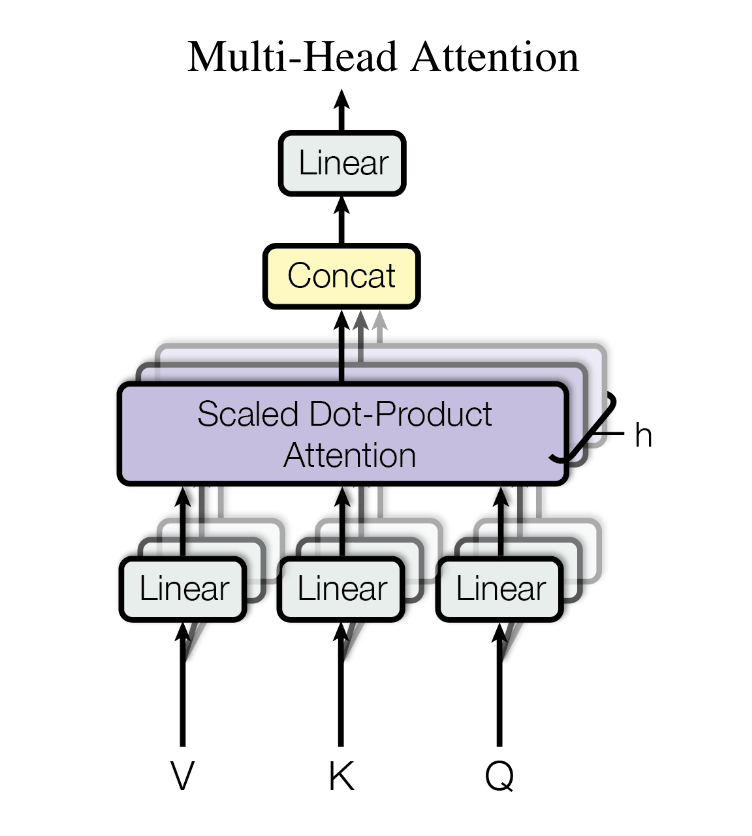
\includegraphics[width=0.6\textwidth]{figures/fig005.png}
    \caption*{Autor:\cite{vaswaniAttentionAllYou2023}}
    \label{fig:fig005}
\end{figure}

O mecanismo de atenção é particularmente chamado de ``Atenção de Produto Escalar Dimensionado'', visto na Figura \ref{fig:fig005}. A entrada consiste em \textit{queries} e chaves de dimensão $d_{k}$ e valores de dimensão $d_{v}$. É calculado os produtos escalares da consulta com todas as chaves e dividido por $\sqrt{d_{k}}$, para fins de controle dos valores em uma menor amplitude. Em seguida, aplica-se uma função \textit{softmax} para obter as probabilidades sobre os valores. Na prática, é calculada a função de atenção em um conjunto de consultas simultaneamente, agrupadas em uma matriz $Q$. As chaves e os valores também são agrupados em matrizes $K$ e $V$. Calcula-se a matriz de saídas como:

\begin{equation}
\text{Attention}(Q, K, V) = \text{softmax}\left(\frac{QK^T}{\sqrt{d_k}}\right)V
\label{eq:attention}
\end{equation}

Dentre os pontos de vantagem do mecanismo de atenção, se destacam: o total de poder computacional por camada, o total de computação que pode ser paralelizada e o poder de capturar a relação de dependência entre dados que se encontram distantes espacialmente um do outro. Como benefício adicional, o mecanismo de atenção pode gerar modelos mais interpretáveis, sob o ponto de vista de como os \textit{tokens} se correlacionam. Não apenas as cabeças de atenção individuais claramente aprendem a executar diferentes tarefas, muitas parecem exibir comportamentos relacionados à estrutura sintática e semântica das frases, no caso da aplicação em \textit{tokens} oriundos de textos.

%--------------------------------------------------------
\section{Otimizador Adam}
\label{sec:adam}

Toda rede neural é treinada aplicando otimização em uma determinada função objetivo afim de minimizar o erro perante os dados de treinamento. Neste contexto, o presente trabalho escolhe o \gls{Adam} como otimizador dada sua adaptatividade.

O método \gls{Adam}, introduzido por \citeonline{kingmaAdamMethodStochastic2014}, é um método popular para o treinamento de modelos de \gls{AP}. O \gls{Adam} combina os benefícios de outras duas técnicas de otimização, o \textit{AdaGrad} e o \textit{RMSProp}. O \gls{Adam} é um método de otimização estocástica eficiente que requer apenas gradientes de primeira ordem com pouca exigência de memória. O método calcula taxas de aprendizado adaptativas individuais para diferentes parâmetros a partir de estimativas dos primeiros e segundos momentos dos gradientes.

Algumas das vantagens do \gls{Adam} podem ser elencadas: taxas de aprendizado adaptativas, que levam a uma convergência mais rápida e eficiente se comparadas com métodos de aprendizado fixos; robustez, que suportam gradientes esparsos de forma efetiva o qual é crucial para diversas aplicações de \gls{AP} atuais; fácil de utilizar, pois requer menos ajustes de parâmetros a tornando amigável ao usuário e acessível a uma grande gama de tarefas.



\chapter{Trabalhos Relacionados} 
\label{chap:trab_relacionados}

% Neste capítulo serão apresentados trabalhos correlatos a este em ordem cronológica de
% publicação. Cada seção é referente a um tópico desta pesquisa, sendo as duas primeiras (Seções
% 3.1 e 3.2), segmentação e classificação, relacionadas a tarefas de visão computacional e divididas entre trabalhos envolvendo a criação de bases de dados (Seções 3.1.1 e 3.2.1) e de modelos
% (Seções 3.1.2 e 3.2.2) para cada um dos tópicos em questão. A Seção 3.3, reconhecimento automático de dor em recém-nascidos, traz algumas das abordagens criadas em função dos anos,
% para contextualização sobre as técnica disponíveis no meio.

Aplicar a unificação de técnicas radiômicas e \textit{deeplearning} em cardiomiopatias já são objeto de estudo em diversas pesquisas recentes.
Neste capítulo serão apresentados trabalhos e metodologias correlatos ao esforço de outros autores a cerca deste tema. As seções se referem a um tópico ou metodologia aplicados nesta pesquisa sendo a primeira (Seção \ref{sec:rev_sistematica}) responsável pela revisão sistemática da literatura.

%---------------------------------------------------------
\section{Revisão Sistemática da Literatura} 
\label{sec:rev_sistematica}

Para a fase exploratória dos trabalhos relacionados, foi utilizada a ferramenta \textit{Parsifal} com o objetivo de identificar estudos onde se aplica a análise radiômica no contexto de cardiopatia. O objetivo inicialmente definido foi o seguinte: "Identificar estudos onde se aplica análise radiômica a cardiopatia. Em segunda opção, alguma outra doença de natureza cardíaca". A pesquisa teve como objetivo responder as seguintes perguntas: quais desafios descritos nos estudos prévios e se há replicabilidade da proposta. As palavras chaves selecionadas são: \textit{cardiac}, \textit{cardiomyopathy} e \textit{radiomics}. A palavra de busca selecionada foi: ``\textit{radiomics} AND (\textit{cardiac} OR \textit{cardiomyopathy})'' com o intuito de filtrar os resultados de forma a identificar onde na ciência poderia identificar a interseção de ambas as abordagens(radiômica e \textit{deep}). Os resultado da busca pode ser conferido na Tabela \ref{tab:resultado_busca}. 

\begin{table}[hbtp]
    \centering
    \renewcommand{\arraystretch}{1.4} % default é 1 
    \begin{tabular}{|c|c|}
    \hline 
          \textbf{Origem} & \textbf{Artigos}  \\ 
    \hline 
        IEEE & 6 \\ 
        PUBMED & 19 \\ 
        Science@Direct & 24 \\ 
    \hline 
    \end{tabular} 
    \caption{Resultados dos Artigos}
    \label{tab:resultado_busca}
\end{table}

Em posse dos resultados, alguns critérios de aceitação foram aplicados como pode ser visto na Tabela \ref{tab:criterios}).

\begin{table}[hbtp]
    \centering
    \caption{Critérios de Inclusão e Exclusão}
    \renewcommand{\arraystretch}{1.4} % default é 1 
    \begin{tabular}{|l|l|}
    \hline 
          \multicolumn{1}{|c|}{\textbf{Critério de Inclusão}} & \multicolumn{1}{c|}{\textbf{Critério de Exclusão}}  \\ 
    \hline 
        \quad Contém ressonância magnética? & \quad Estudos Duplicados   \\ 
        \quad O objeto de estudo é o coração? & \quad Estudos Secundários ou Terciários \\
        \quad Usa análise de textura? & \quad Estudos que não estão em PT ou EN\\
        \quad Utiliza análise radiômica? & \quad Leitura cinza  \\
        \quad É cardiomiopatia? & \quad Não aplica técnicas computacionais\\
        & \quad Não trata do coração \\
        & \quad Não usa RM \\
        & \quad Trabalho que atua somente com dados genômicos \\ 
    \hline 
    \end{tabular} 
    \caption*{Fonte: Autor}
    \label{tab:criterios}
\end{table}

Critérios de aceitação também foram aplicados e podem ser conferidos na Tabela \ref{tab:questoes}. Dentre cada uma das seis perguntas, calculamos a nota usando como pontuação 1 para sim, 0,5 para parcial e 0 para talvez. Como nota de corte usamos o valor 3, ou seja, qualquer artigo que não alcance o valor mínimo de 3, é descartado. Uma vez aplicado os critérios de aceitação, restaram 18 artigos dos 49 artigos iniciais.

\begin{table}[hbtp]
    \centering
    \caption{Questões de Aceitação}
    \renewcommand{\arraystretch}{1.4} % default é 1 
    \begin{tabular}{|l|}
    \hline 
          \multicolumn{1}{|c|}{\textbf{Questões}} \\ 
    \hline 
        \quad É descrita as limitações do estudo? \\
        \quad Há um experimento bem descrito para avaliar a proposta? \\
        \quad Há mais de 2 autores? \\
        \quad O trabalho apresenta resultados? \\
        \quad A introdução apresenta o problema de forma clara \\
        \quad É análise sistemática da literatura? \\
    \hline 
    \end{tabular} 
    \caption*{Fonte: Autor}
    \label{tab:questoes}
\end{table}

Um esquemático de como o processo foi feito, bem como sua seleção e critérios aplicados, podem ser conferidos na Figura \ref{fig:fig021}.

\begin{figure}[htbp]
    \centering
    \caption{Representação de Funil da Seleção da Literatura}
    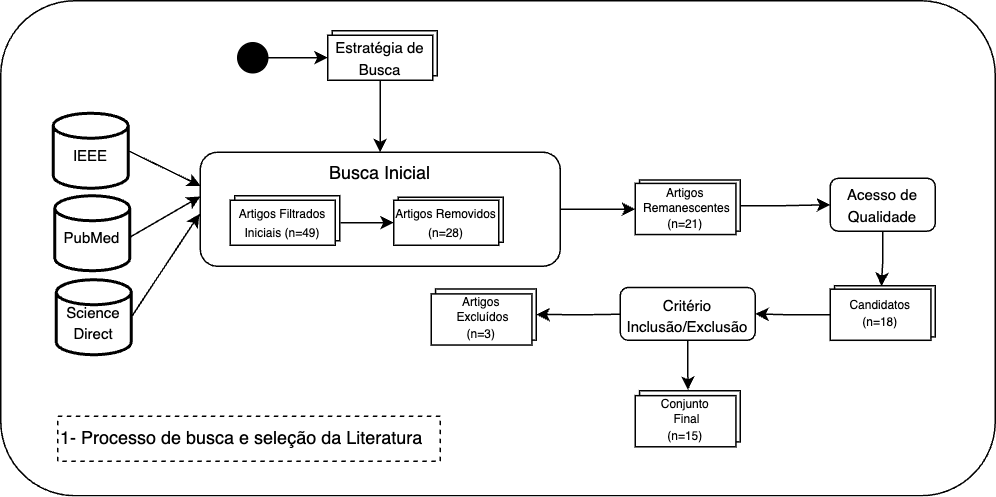
\includegraphics[width=0.8\textwidth]{figures/fig021.png}
    \caption*{Fonte: Autor}
    \label{fig:fig021}
\end{figure}
%---------------------------------------------------------
\section{Análise Radiômica com Atenção}
\label{sec:analise_radiomica}

 \citeauthor{jiangMRIBasedRadiomics2021} \citeyear{jiangMRIBasedRadiomics2021} conduziram um estudo abrangente que aproveita as capacidades do aprendizado de máquina para melhorar os processos diagnósticos em oncologia, especificamente focando no câncer de colo de útero em estágio inicial. Sua pesquisa, intitulada "Abordagem Radiômica Baseada em Ressonância Magnética com Aprendizado Profundo para Predição de Invasão Vascular em Câncer de Colo de Útero em Estágio Inicial", foca na aplicação de técnicas de aprendizado profundo em dados de ressonância magnética multiparamétrica para prever a invasão vascular, um fator crítico para determinar a agressividade do câncer de colo de útero e informar estratégias de tratamento.

O estudo utilizou um conjunto substancial de dados compreendendo 1.070 imagens de ressonância magnética com contraste dinâmico T1 (DCE-T1) e 986 imagens de ressonância magnética ponderada em T2 (T2WI) coletadas de 167 pacientes diagnosticadas com câncer de colo de útero em estágio inicial entre janeiro de 2014 e agosto de 2018. Os pesquisadores empregaram uma nova estrutura de aprendizado profundo que integrou esses dois tipos distintos de varreduras em imagens RM para criar um modelo preditivo robusto. Implementando uma estratégia de aprendizado de conjunto com atenção, o modelo efetivamente distinguiu entre casos com invasão vascular e aqueles sem. Quatro modelos de CNN foram utilizados: VGGNet, GoogLeNet (Inception-v3), Residual Network (ResNet) e DenseNet. Um módulo padrão de \gls{SE}  e o módulo de atenção de bloco convolucional, do termo inglês \gls{CBAM},  foram introduzidos após cada bloco de convolução da rede \textit{AdaptedVGG19} para fornecer um \textit{AdaptedVGG19-SE} e um \textit{AdaptedVGG19-CBAM}, respectivamente. A arquitetura proposta é vista na Figura. \ref{fig:fig007}.

O desempenho preditivo dos modelos foi rigorosamente avaliado usando a área sob a curva (ROC), com os modelos finais alcançando uma alta área sob a curva (AUC) de 0.911. Essa alta AUC indica uma forte capacidade do modelo para classificar corretamente a presença ou ausência de invasão vascular, com métricas de sensibilidade e especificidade também demonstrando precisão diagnóstica substancial.

Esta pesquisa demonstra o potencial de integrar algoritmos de aprendizado profundo com dados de imagem complexos para melhorar as avaliações diagnósticas pré-operatórias. Os achados de \citeauthor{jiangMRIBasedRadiomics2021} sugerem que tais abordagens analíticas avançadas podem fornecer suporte substancial na tomada de decisões clínicas, potencialmente levando a planos de tratamento mais personalizados e melhores resultados para os pacientes.

No contexto da pesquisa contínua em imagens médicas e diagnóstico de câncer, a metodologia e os resultados de \citeauthor{jiangMRIBasedRadiomics2021} fornecem um exemplo convincente do potencial da inteligência artificial para revolucionar os processos diagnósticos em oncologia. O uso de ressonância magnética multiparamétrica e modelos sofisticados de aprendizado de máquina exemplifica as abordagens inovadoras que estão sendo desenvolvidas para enfrentar os desafios da detecção precoce e precisa de câncer.

\begin{figure}[htbp]
    \centering
    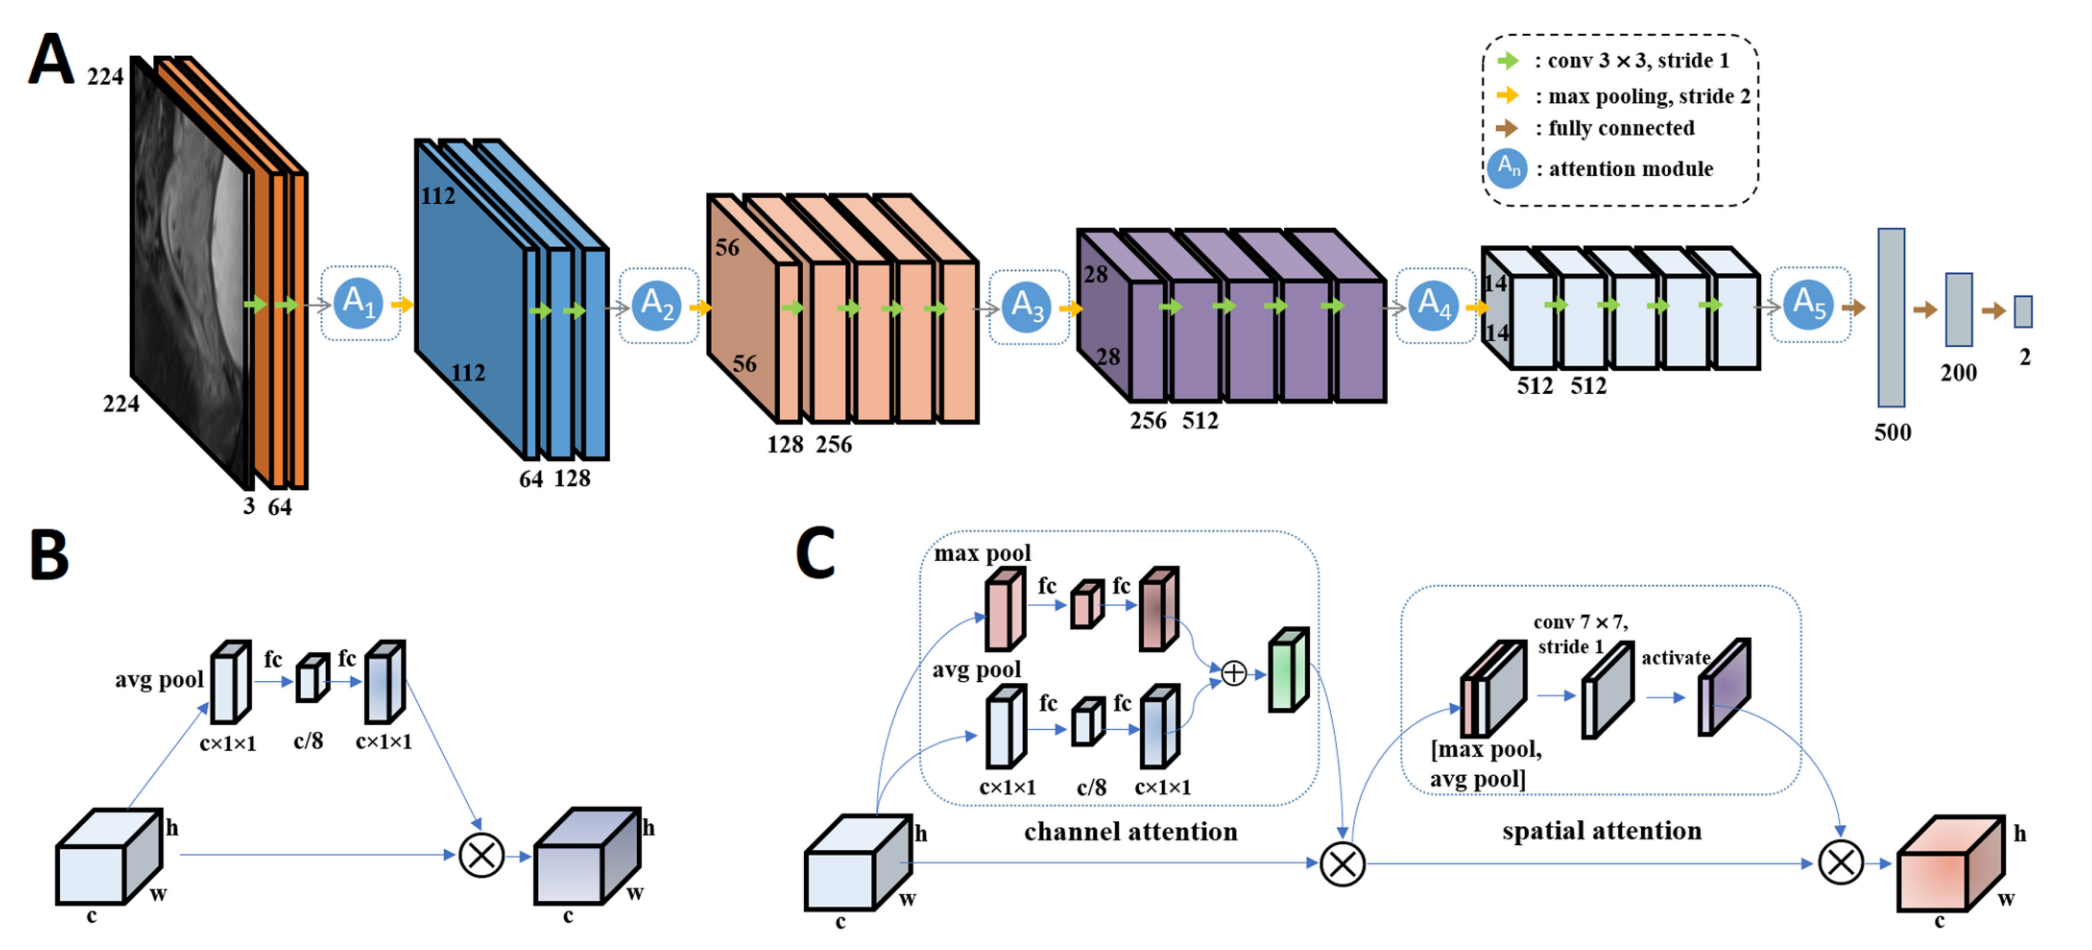
\includegraphics[width=0.8\textwidth]{figures/fig007.png}
    \caption{Fonte: \cite{jiangMRIBasedRadiomics2021}}
    \label{fig:fig007}
\end{figure}

%---------------------------------------------------------
Em outro trabalho, \cite{renBiLSTMMultiheadAttentionbased2023} desenvolveram um modelo avançado usando uma rede Bi-LSTM (memória de longo prazo bidirecional) combinada com um mecanismo de atenção de múltiplas cabeças, utilizando \textit{features} radiômicas e imagens TC de lesões, para aprimorar a diferenciação dos principais subtipos de adenocarcinoma pulmonar, integrando assinaturas radiômicas com características radiológicas de tomografias computadorizadas. O estudo recrutou 421 pacientes de três hospitais, confirmados com adenocarcinoma in situ, adenocarcinoma minimamente invasivo ou adenocarcinoma invasivo, com base na análise de 427 lesões.

A metodologia empregada envolveu a extração de assinaturas radiômicas usando o software `\textit{PyRadiomics}' das regiões de lesões identificadas em cada imagem de tomografia computadorizada. As 100 principais características foram então selecionadas através do método de classificação de características de máxima relevância e mínima redundância. Um modelo preditivo foi subsequentemente desenvolvido empregando essas características juntamente com características radiológicas, usando a estrutura Bi-LSTM e atenção múltipla para classificar as lesões.

O desempenho diagnóstico do modelo foi quantitativamente impressionante, alcançando valores da área sob a curva (AUC) de 0,985, 0,94 e 0,981 nos grupos de treinamento, teste e validação, respectivamente, com precisões correspondentes de 0,92, 0,976 e 0,91. Além disso, comparações foram feitas com dois outros modelos — rede neural convolucional (CNN) + atenção múltipla, e LSTM + atenção múltipla — demonstrando que o modelo Bi-LSTM e atenção múltipla superou essas alternativas em precisão e acurácia no conjunto de testes.

Esta pesquisa destaca a utilidade potente da combinação de técnicas avançadas de aprendizado de máquina com análises radiômicas e radiológicas detalhadas para refinar o processo diagnóstico para subtipos de adenocarcinoma pulmonar, potencialmente orientando abordagens de tratamento mais personalizadas baseadas na caracterização do subtipo.

%---------------------------------------------------------
 \cite{aiSelfAttentionBasedFusion2023} conduziram um estudo inovador intitulado ``Um Modelo de Fusão Baseado em Autoatenção de Características Radiômicas e Profundas para Previsão de Recorrência Precoce em CPNP'', que aborda o significativo desafio de prever a recorrência precoce em câncer de pulmão de células não pequenas usando técnicas avançadas de aprendizado de máquina. Sua pesquisa aproveita o mecanismo de autoatenção para fundir características radiômicas manuais e características de aprendizado profundo extraídas de imagens de TC, com o objetivo de aumentar a precisão preditiva e robustez para recorrência precoce em câncer de pulmão de células não pequenas.

O estudo começou empregando diversas técnicas de aprendizado de máquina para extrair uma variedade de características artesanais de imagens de TC, incluindo atributos de textura, forma e escala de cinza. Para capturar informações semânticas de alto nível e de representação, uma rede ResNet50 pré-treinada foi utilizada para a extração de \textit{features} profundas. Essas características extraídas foram então fundidas com um vetor de características extraído de dados de texturas de imagens radiômicas e unificado usando um módulo de fusão de autoatenção inovador desenvolvido pelos pesquisadores. Este módulo otimiza e pondera o vetor de características fundidas, aproveitando plenamente o mecanismo de autoatenção para melhorar as capacidades de previsão do modelo. A arquitetura pode ser conferida na Figura \ref{fig:fig008}.

Os resultados experimentais, avaliados no conjunto de dados público Cancer Imaging Archive (TCIA), demonstraram que o modelo proposto superou significativamente os métodos existentes na previsão de recorrência precoce. O modelo exibiu melhorias substanciais em precisão de classificação, sensibilidade, especificidade e a área sob a curva (AUC), destacando seu potencial para guiar o tratamento em estágio inicial e melhorar as taxas de sobrevivência para pacientes com câncer de pulmão de células não pequenas.

Este estudo exemplifica a aplicação de técnicas avançadas de aprendizado de máquina em imagens médicas e oncologia, fornecendo um método robusto para a previsão de recorrência precoce que poderia impactar significativamente os resultados clínicos e as estratégias de tratamento em câncer de pulmão.

\begin{figure}[htbp]
    \centering
    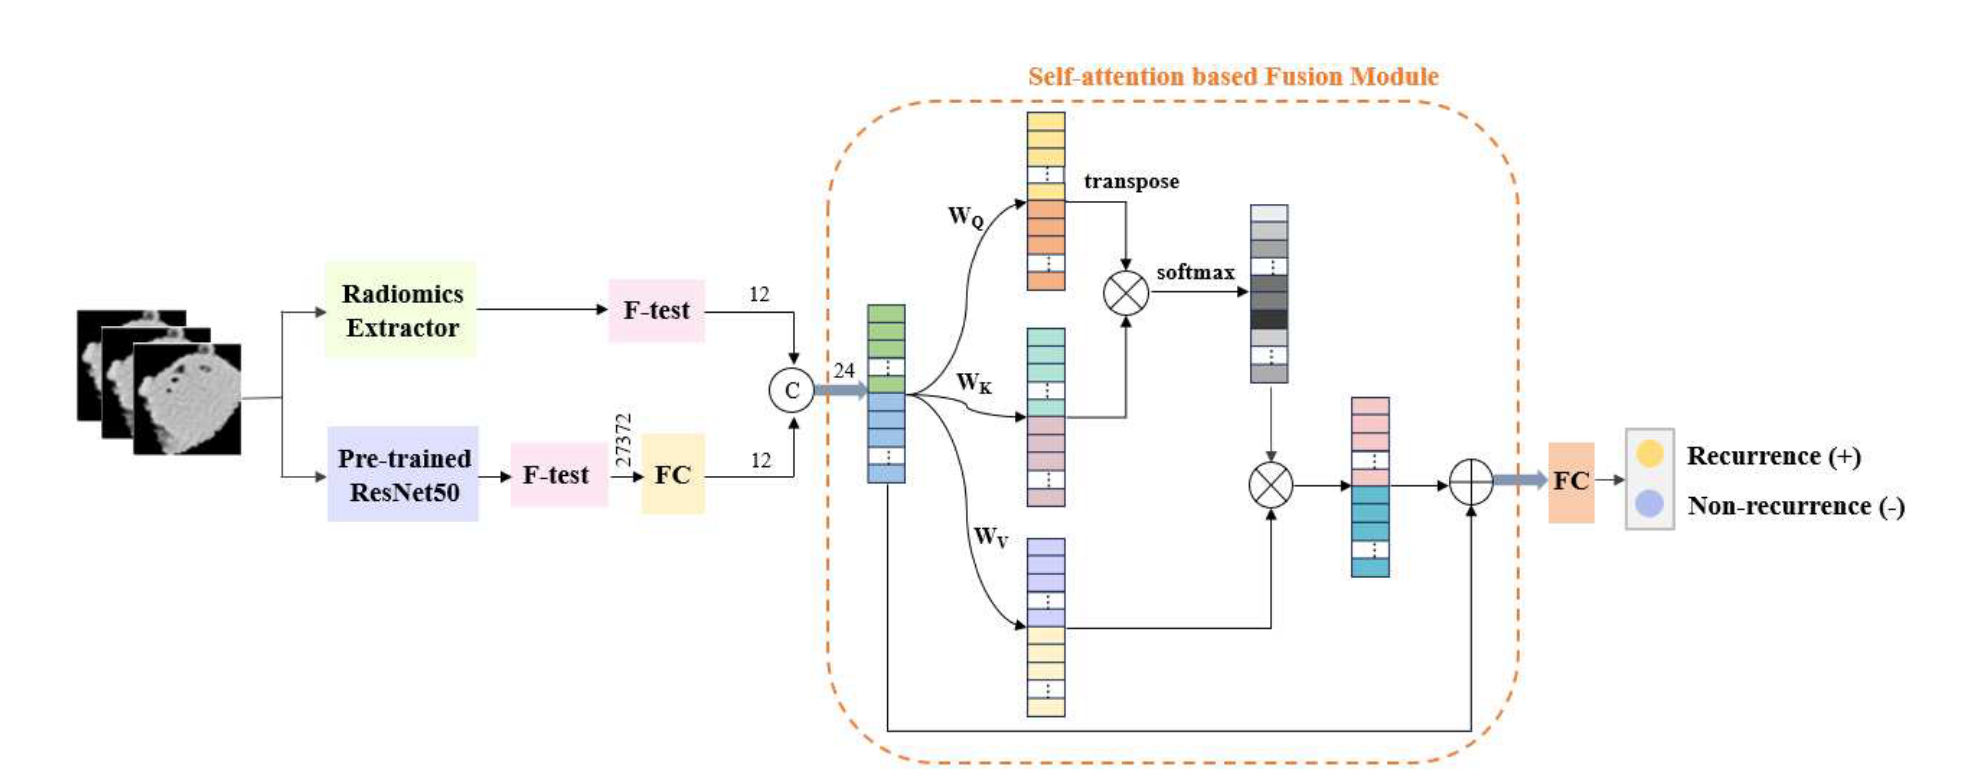
\includegraphics[width=1\textwidth]{figures/fig008.png}
    \caption{Fonte: \cite{aiSelfAttentionBasedFusion2023}}
    \label{fig:fig008}
\end{figure}
%---------------------------------------------------------

\cite{iranmehrImprovedPredictionMGMT2022} desenvolveram uma rede de aprendizado profundo inovadora que utiliza um mecanismo baseado em atenção para aprimorar a previsão do estado de metilação do gene MGMT em glioblastoma muiltifoma (GBM), o tipo mais agressivo de tumor cerebral. Pacientes com GBM possuem uma expectativa muito baixa, entre 18 e 24 meses e requerem tratamentos agressivos, como por exemplo, quimioterapia. Sua pesquisa, apresentada em "Improved Prediction of MGMT Methylation Status in Glioblastoma using a Deep Attention Network", destaca um avanço significativo nas capacidades diagnósticas não invasivas para GBM, que tipicamente tem uma taxa de sobrevivência de apenas 18 meses.

O estudo foca no gene MGMT, cujo estado de metilação é crucial para determinar a eficácia da quimioterapia em pacientes com GBM. As análises radiômicas tradicionais, embora úteis, muitas vezes não capturam os recursos intrincados necessários para uma previsão precisa da metilação. \citeauthor{iranmehrImprovedPredictionMGMT2022} propõem um modelo que integra características radiômicas manuais com técnicas de aprendizado profundo, melhorando a extração de características e a precisão da previsão de GBM.

O modelo introduzido pela equipe utiliza uma combinação de mecanismos de atenção \textit{squeeze} e sequencial para priorizar fatias e regiões relevantes dentro das imagens de ressonância magnética, respectivamente. Esse método não apenas melhora o foco em áreas significativas, mas também aprimora a interpretabilidade geral do modelo. O modelo proposto (Fig. \ref{fig:fig009}) consiste de três etapas: 1) Um modelo base para extrair as \textit{features}, 2) uma rede de atenção temporal e espacial e 3) uma rede de classificação para prever se o exame é metilado ou não metilado. 

\begin{figure}[htbp]
    \centering
    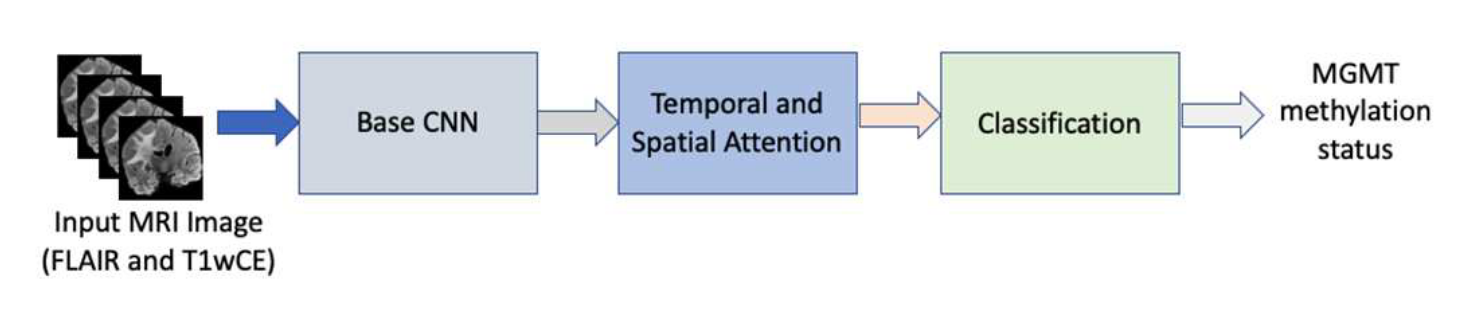
\includegraphics[width=1\textwidth]{figures/fig009.png}
    \caption{Método proposto. \textit{Densenet} foi utilizado como modelo base. A saída da rede densa é alimentada pela rede de atenção que pode priorizar as fatias e regiões. A saída da rede de atenção é enviada à rede de classificação binária para prever o status de metilação do MGMT.}
    \label{fig:fig009}
\end{figure}

O modelo base consiste em uma \textit{DenseNet}. Segundo o autor, a \textit{Densenet} pode suportar milhares de camadas e ser resistente ao \textit{overfitting}. A saída da rede densa é fornecida para a rede de \textit{squeeze} e \textit{self-attention} conforme mostrado na Fig. \ref{fig:fig010}. Cada exame consiste em várias fatias e a \textit{squeeze attention} priorizará as fatias, usando o agrupamento médio global seguido por duas camadas densas separadas e depois o produto escalar com a entrada inicial. A saída da \textit{squeeze attention} é fornecida à rede de \textit{self-attention}. Após a aplicação da \textit{self-attention}, o mapa de atenção contém pixels com uma seção de maior importância em cada fatia. Com a rede de \textit{self-attention}, é possível enfatizar pixels e regiões de diferentes independente da distância em que estes \textit{pixels} se localizam pela imagem. Múltiplas regiões com diferentes tamanhos geradas a partir de regiões integrais são então fornecidas à \textit{attention} sequencial (SA). A rede SA adapta uma rede \textit{long short term memory} (LSTM), que é capaz de aprender dependências de longo prazo. A saída passa por uma camada densa e uma sigmoide para fazer a classificação.

Avaliado em várias métricas de classificação binária, o modelo alcançou a melhor área sob a curva (AUC) de 70,59, demonstrando sua superioridade em relação aos métodos existentes. Este trabalho fornece uma abordagem robusta e automática para capturar características críticas de imagens de ressonância magnética, avançando significativamente na previsão do estado de metilação em GBM em comparação com métodos anteriores. As implicações de tais avanços são profundas, potencialmente melhorando o planejamento de tratamentos personalizados e, em última análise, os resultados para os pacientes com glioblastoma.

\begin{figure}[htbp]
    \centering
    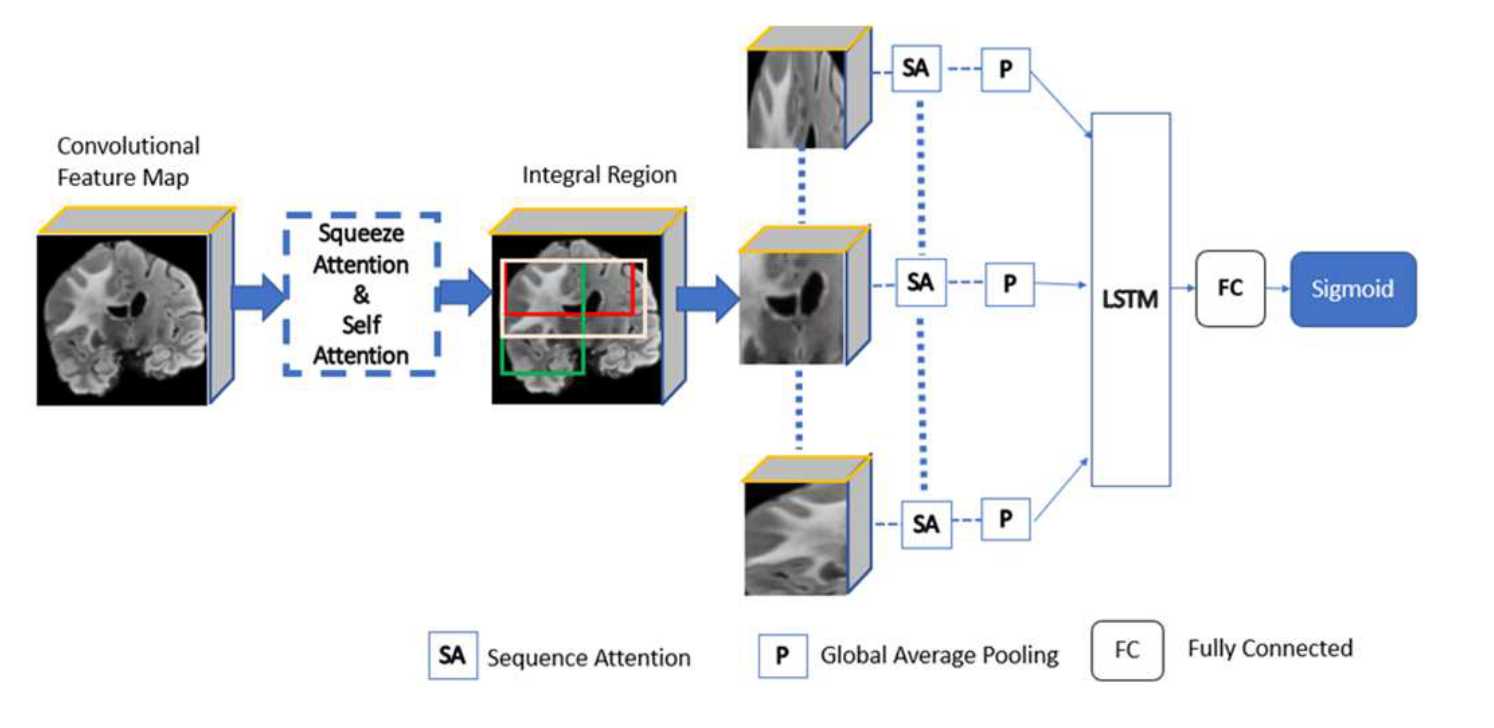
\includegraphics[width=1\textwidth]{figures/fig010.png}
    \caption{Fonte: \cite{iranmehrImprovedPredictionMGMT2022}}
    \label{fig:fig010}
\end{figure}

%---------------------------------------------------------
% \section{Considerações Finais do Capítulo}
% \label{sec:rcond_cap_3}
% \lipsum[2-4]
\chapter{Metodologia} 
\label{chap:metodologia}

O objetivo deste trabalho é propor e investigar uma arquitetura de aprendizado profundo que unifica características radiômicas e características profundas. Inicialmente, é empregado diversas técnicas de aprendizado de máquina para extrair características manuais de imagens de RM, abrangendo textura, forma, escala de cinza, etc. Posteriormente, uma rede \textit{ResNet50} pré-treinada é utilizada para extrair características profundas que encapsulam informações semânticas de alto nível e de representação das imagens de \gls{RMC}. Estas características são então fundidas em um vetor de características unificado. Para aprimorar a acurácia e a robustez, um módulo de \textit{self-attention} foi desenvolvido, utilizando o mecanismo de autoatenção, este módulo otimiza e pondera o vetor de características fundidas de forma eficaz.

%---------------------------------------------------------
\section{Métodos}
\label{sec:cap4_metodos}

 %  @TODO Muedar seções e subsessões. pag - 32
 %  @TODO Muedar Texto Resnet abaixo também mediante correção pag - 32

%---------------------------------------------------------
\subsection{ResNet}
\label{subsec:cap4_resnet}

A \textit{ResNet} (Rede Residual) é uma arquitetura de rede neural profunda amplamente utilizada em tarefas de visão computacional, como classificação de imagens, detecção de objetos e segmentação de imagens. Ela foi introduzida por  \cite{heDeepResidualLearning2015}, e se destacou por ganhar a competição ImageNet em 2015 com uma precisão significativamente maior do que as arquiteturas anteriores. A principal característica da \textit{ResNet} é sua capacidade de treinar redes muito profundas sem sofrer com o problema do "desvanecimento do gradiente" que afeta principalmente redes neurais profundas e impede o treinamento de progredir por conta de valores muito baixos de gradiente, problema este muito comum em redes tradicionais muito profundas. A \textit{ResNet} introduz um conceito chave chamado bloco residual que é um componente da rede onde a entrada do bloco é somada à sua saída antes de passar para a próxima camada. Esta conexão direta é chamada de \textit{skip connection} ou \textit{short-cut connection} e pode ser conferida na Figura 11.

\begin{figure}[htbp]
    \centering
    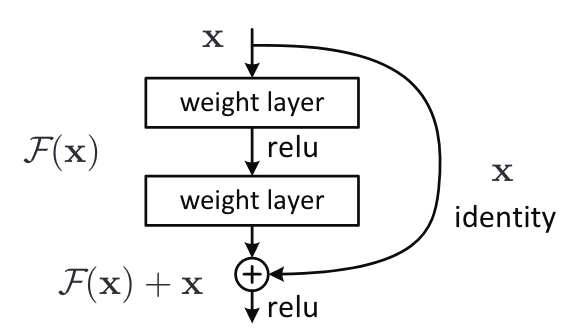
\includegraphics[width=0.6\textwidth]{figures/fig013.png}
    \caption{Fonte: \cite{aiSelfAttentionBasedFusion2023}}
    \label{fig:fig013}
\end{figure}

A ResNet é composta por vários blocos residuais empilhados.
Existem várias versões da \textit{ResNet}, como \textit{ResNet}-18, \textit{ResNet}-34, \textit{ResNet}-50, \textit{ResNet}-101, e \textit{ResNet}-152, onde os números indicam a profundidade total da rede, ou seja, o número de camadas).
% A \textit{ResNet}, desenvolvidas por \cite{heDeepResidualLearning2015}, são arquiteturas convolucionais formada pela composição de blocos residuais, seguidos de uma camada completamente conectada. Estes blocos, ilustrados na Figura 11, empregam o que os autores chamam de \textit{skip connections}, conexões que permitem que camadas sejam puladas durante o treino, resolvendo o problema conhecido como \textit{vanishing gradient}, que afeta principalmente redes neurais profundas e impede o treinamento de progredir por conta de valores muito baixos de gradiente. A inovação trazida por este modelo permitiu a criação de redes muito mais profundas e pode possuir um número definido de camadas, portanto o uso de nomes como ResNet50 ou ResNet101 é uma prática comum para identificar a quantidade de camadas utilizadas no modelo.

%---------------------------------------------------------
\subsection{Features Radiômicas}
\label{subsec:cap4_features_radiomicas}

Serão extraídas características radiômicas de fase diastólica, representada por um conjunto de fatias variando entre 6 e 18 \textit{frames}, de cada paciente usando \gls{GLCM} e estatísticas baseadas em histograma. Será aplicado o filtro \gls{LoG} com cinco valores diferentes em cada parte para suavizar as imagens e realçar as bordas. Foi calculado características \gls{GLCM} como contraste, entropia, correlação, homogeneidade e energia para cada filtro \gls{LoG}. Também é calculado características de intensidade como média, variância, média dos percentis (10 e 90), desvio robusto da média absoluta, curtose e assimetria usando estatísticas de primeira ordem. Foram obtidos 78 características radiômicas para cada paciente dentro da quantidade de fatias extraídas na fase diastólica.

% @TODO - Fase diastólica explicar pag - 33

%---------------------------------------------------------
\subsection{Features Profundas}
\label{subsec:cap4_features_profundas}
 
Para extrair características profundas das imagens de \gls{RMC}, é utilizada a arquitetura pré-treinada de um \textit{ResNet50} sem sua última camada totalmente conectada, treinada no conjunto de dados \textit{ImageNet}. Estudos anteriores demonstraram que o pré-treinamento com \textit{ImageNet} pode melhorar o desempenho de tarefas de classificação de imagens médicas. \textit{ResNet50} é um modelo de rede neural convolucional profunda com 50 camadas que compreende muitos blocos residuais. Cada bloco contém módulos de convolução e uma conexão de salto que transfere a informação do bloco anterior para o próximo bloco. A conexão de salto ajuda a reter a informação semântica mais básica aprendida nas camadas anteriores, que de outra forma se tornaria abstrata devido à conexão de longa cadeia. A conexão de salto também evita o desaparecimento do gradiente nas camadas mais profundas ao fornecer um caminho alternativo para a retropropagação. A informação da conexão de salto é adicionada à informação calculada em cada bloco \cite{aiSelfAttentionBasedFusion2023}. Ao todo são 2048 características coletadas da saída deste modelo.

%---------------------------------------------------------
\subsection{Unificando as Features}
\label{subsec:cap4_unificando_features}

Um vez em posse das features radiômicas, é aplicado um \textit{F-Test} tanto às 78 características radiômicas quanto às 2048 características profundas, reduzindo cada um dos vetores ao espaço de 64 características. No método de fusão convencional, simplesmente é concatenado os dois vetores de características como na Eq. \ref{eq:concat}, onde \textit{Concat} simplesmente concatena os dois vetores. Unificando ambos os vetores obtemos o valor resultante de 128 características o qual será enviado ao mecanismo de autoatenção.

\begin{equation}
F_{hd} = \textit{Concat}(F_h, F_d)
\label{eq:concat}
\end{equation}

%---------------------------------------------------------
\subsection{Módulo de Fusão de Autoatenção}
\label{subsec:cap4_mod_self_attention}

Neste trabalho é empregado o mecanismo de autoatenção para aprender a importância de cada característica e capturar suas dependências de longo alcance. Como ilustrado na Figura \ref{fig:fig011}, o módulo de fusão de autoatenção é utilizado para mapear uma consulta ($Q$), chave ($K$) e valor ($V$) para um valor de atenção. São utilizadas as 128 características concatenadas $F_{hd}$  como \textit{tokens} e projetada cada característica em três matrizes aprendíveis: matriz chave $K$, matriz consulta $Q$ e matriz de valor $V$ por produto escalar com as matrizes $W_{Q}$, $W_{K}$ e $W_{V}$. Logo os valores $Q$, $K$, $V$ são denotados como $W_{Q}F_{gd}$, $W_{K}F_{gd}$, $W_{V}F_{gd}$ respectivamente, onde $W_{Q}$, $W_{K}$ e $W_{V}$ representam a transformação linear para as matrizes $Q$, $K$ e $V$. O módulo de fusão baseado em autoatenção é definido como segue na Equação \ref{eq:attention}, onde $d_{k}$ é a dimensão do valor de $K$. Sem utilizar operações recorrentes ou convolucionais, o módulo de fusão de autoatenção pode modelar as dependências de longo prazo entre as características de entrada.      Este módulo calcula de forma adaptativa os pesos entre as características com base em sua importância e relevância, capturando de forma mais abrangente as associações entre características radiômicas e profundas. Tal processo realça a capacidade expressiva das características fundidas e permite que o modelo foque mais precisamente nas características mais informativas para prever \gls{CH} e reduzir a influência de características irrelevantes na previsão. Além disso, o modelo pode alocar dinamicamente atenção a diferentes amostras de imagens de \gls{RMC}. Essa flexibilidade permite com que o modelo se adapte melhor à representação de características de diferentes amostras, melhorando a precisão e a generalização da previsão.

%---------------------------------------------------------
\subsection{Função de Perda}
\label{subsec:cap4_funcao_perda}

A função de perda utilizada utilizada no modelo é a função de entropia cruzada binária, do termo  \gls{BCE}, que é calculada pela Eq. \ref{eq:bce} onde $\mathcal{L}_{bce}$ denota o \gls{BCE}, $N$ denota o número de imagens de \gls{RMC}, $r$ denota a classe alvo de \gls{CH} e $\hat{r}$ o valor previsto pelo modelo de \gls{CH}, 1 indica indícios de \gls{CH} e 0 sua ausência.

\begin{equation}
\mathcal{L}_{bce} = -\frac{1}{N} \sum_{i=1}^N
(r_i \ln \hat{r}_i + (1 - r_i) \ln (1 - \hat{r}_i))
\label{eq:bce}
\end{equation}

%---------------------------------------------------------
\subsection{Arquitetura Proposta}
\label{subsec:cap4_arquitetura_proposta}

O esquemático da arquitetura proposta pode ser conferida na Figura \ref{fig:fig011}. A imagens de \gls{RMC} são expostas ao seletor de características via \textit{F-test}, as características selecionadas são concatenadas e enviadas ao módulo de fusão de autoatenção, por fim uma camada linear de 128 características precede um camada linear com um único neurônio para a classificação binária.

% @TODO Mover essa parte. pag - 35

\begin{figure}[htbp]
    \centering
    \caption{Arquitetura Proposta}
    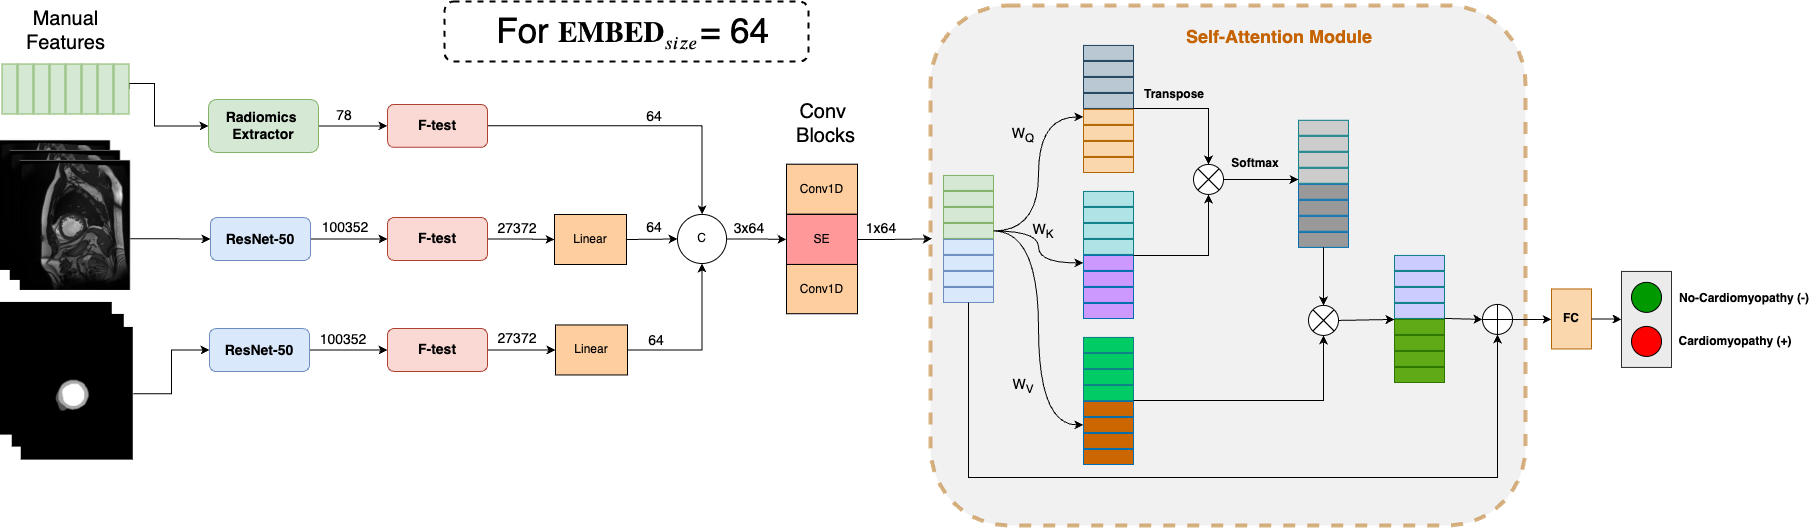
\includegraphics[width=1\textwidth]{figures/fig011.png}
    \caption*{Fonte: Autor}
    \label{fig:fig011}
\end{figure}

Para medir o desempenho da solução serão aplicadas as seguintes métricas: acurácia e precisão, expressas pelas equações \ref{eq:acc}, \ref{eq:precision} e \ref{eq:recall}.
Também é calculada a \gls{AUC}, também reconhecida como a área que avalia o modelo em diversos limites contínuos de decisão, verificando a taxa de verdadeiros positivos contra falsos positivos em cada limite.

% A precisão foi escolhida neste contexto pois quanto maior esta for, menor é a taxa de falso negativo nos resultados. A precisão é pertinente quando o custo com a identificação de falso positivos é alto, como é o caso de doenças fatais.

\begin{equation}
\textit{Acurácia} = \frac{\textit{TP} + \textit{TN}}{\textit{TP} + \textit{TN} + \textit{FP} + \textit{FN}}
\label{eq:acc}
\end{equation}

\begin{equation}
\textit{Precisão} = \frac{\textit{TP}}{\textit{TP} + \textit{FP}}
\label{eq:precision}
\end{equation}

\begin{equation}
\textit{Revocação} = \frac{\textit{TP}}{\textit{TP} + \textit{FN}}
\label{eq:recall}
\end{equation}

%---------------------------------------------------------
% \subsection{Unificando as Features}
% \label{subsec:cap4_unificando_features}

% Um vez em posse das features radiômicas, é aplicado um F-Test e reduz-se cada um dos vetores à 64 características. Unificando ambos os vetores obtemos um vetor de características de tamanho 128 o qual passará pelo mecanismo de \textit{attention}.

%---------------------------------------------------------
\subsection{Fluxograma}
\label{subsec:cap4_floxugrama}

A Figura \ref{fig:fig015} confere o fluxograma do projeto ilustrando de forma esquemática suas fases de atuação.

% @TODO Mover essa parte. pag - 36

\begin{figure}[htbp]
    \centering
    \caption{Fluxograma do Projeto}
    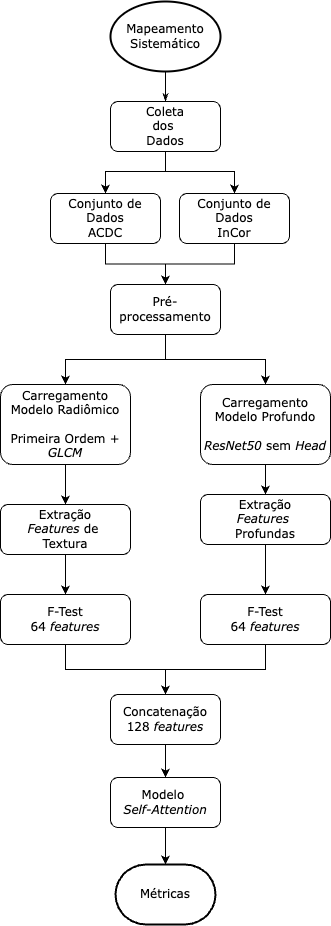
\includegraphics[width=0.4\textwidth]{figures/fig015.png}
    \caption*{Fonte: Autor}
    \label{fig:fig015}
\end{figure}

% @TODO Acrescentar dados Incor e ACDC. pag - 37


%---------------------------------------------------------
\section{Considerações Finais do Capítulo}
\label{sec:cap4_consideracoes_finais}

Como considerações, destacam-se o uso de base de dados pública, com dados de pacientes incluindo o conjuntos de fatias que identificam a ação de sístole e diástole do coração. É aplicado pré-processamento do qual é extraído manualmente 78 características radiômicas, características estas que analisam textura, níveis e variações dos tons de cinza incluindo diversas estatísticas como de primeira ordem e o \gls{GLCM}. Ainda em fase de pré-processamento é extraída as características profundas oriundas do modelo de visão \textit{ResNet50}, com os pesos treinados na base de dados da \textit{ImageNet}. É removida a última camada linear da \textit{ResNet50} resultando ao seu final, sem a camada classificadora, 2048 características. Em posse de ambas as features, é aplicada a técnica de \textit{F-test} para obter as 64 características mais relevantes e, após, concatená-las obtendo um vetor de características de 128 características. Este vetor é exposto ao módulo de fusão com autoatenção, identificando as características mais determinantes independente de espacialidade. 
\chapter{RESULTADOS E DISCUSSÕES}
\label{chap:proposta_experimental}

Este capítulo traz informações relacionadas com as ferramentas utilizadas no experimento, como linguagem, bibliotecas utilizadas, entre outros. Assim como, informações sobre o consumo de dados das bases \gls{ACDC} e SunnyBrook, fase de pré-processamento, inferência nos modelos implementados, sendo estes, modelo linha de base e derivados, e modelos adaptados. Por fim, são apresentados os resultados considerando as métricas apresentadas na seção \ref{subsec:cap4_metrics} utilizando as bases de dados ACDC e SunnyBrook e cada uma das abordagens: o modelo base e o modelo proposto.

Por fim, este capítulo apresenta os resultados da prova de conceito realizada com os algoritmos desenvolvidos, tanto o modelo base quanto os modelos adaptados, com o intuito de compará-los aos objetivos traçados nesta dissertação. Os testes realizados buscam avaliar a eficiência do algoritmo sob as diversas adaptações discutidas. 

%--------------------------------------------------------
\section{MATERIAIS} 
\label{sec:cap5_materiais}

A Tabela \ref{tab:hardware_software} apresenta as ferramentas que foram utilizadas nesse projeto. Destaca-se que foram utilizadas majoritariamente ferramentas open-source como a linguagem \textit{python}, bibliotecas como \textit{pyradiomics}, \textit{torch}, \textit{numpy}, entre outras. Para registro dos experimentos, foi utilizada a ferramenta CometML\footnote{https://www.comet.com}. No CometML é possível armazenar valores como: erro do lote no treinamento, acurácia do conjuntos de validação no treinamento, métricas resultantes como acurácia, hiperparâmetros como taxa de aprendizado, épocas, etc.
\newline

\begin{table}[hbtp]
    \caption{Fonte: Componentes Utilizados}
    \centering
    \renewcommand{\arraystretch}{1} % default é 1 
    % \begin{tabular}{|>{\centering\arraybackslash}p{2cm}|p{12cm}|}
    \begin{tabular}{|c|c|}
    \hline 
       \textbf{Item} & \textbf{Descrição}\\
    \hline 
       Computador & \textit{Macbook M1 Pro}  \\
    \hline 
       Memória & 16gb  \\
    \hline 
       Versão \textit{Python} & 3.11.0  \\
    \hline 
       Versão \textit{pyradiomics} & 3.0.1 \\
    \hline 
       Versão \textit{torch} & 2.2.1 \\
    \hline 
       Versão \textit{torchvision} & 0.17.1 \\
    \hline 
       Versão \textit{numpy} & 1.26.4 \\
    \hline 
       Versão \textit{scikit-learn} & 1.4.1.post1 \\
    \hline 
       Versão \textit{comet-ml} & 3.47.4 \\
    \hline 
    \end{tabular} 
    \caption*{Fonte: Autor}
    \label{tab:hardware_software}
\end{table}

%--------------------------------------------------------
\section{CENÁRIOS DE TESTE} 
\label{subsec:cap5_dataset}

Este trabalho visou realizar os experimentos em duas bases distintas com imagens de \gls{RMC}, informações a cerca do paciente e rótulos que indicam presença ou não de cardiomiopatia. Testes iniciais foram feitos no conjunto de dados \gls{ACDC} que possui $30$ casos de \gls{CMH}, $30$ casos de \gls{CMD} e $90$ casos sem cardiomiopatia, resultando em $60$ casos de cardiomiopatia e $90$ casos sem cardiomiopatia. Da base \gls{ACDC} se pretende utilizar apenas as fatias da fase diastólica. O segundo conjunto de dados é o \textit{SunnyBrook}, possuindo imagens na fase diastólica contendo as classes $9$ classes NOR (sem cardiomiopatia) e $12$ HIP (hipertrofia do ventrículo esquerdo).

O modo de operação será o mesmo para ambos os conjuntos de dados com exceção do pré-processamento dado ao fato da forma como o conjunto de dados \textit{SunnyBrook} disponibiliza as máscaras.

Por fim, foram realizados três testes: 1) utilizando o modelo base no conjunto de dados do ACDC; 2) utilizando o modelo adaptado no conjunto de dados do ACDC; 3) utilizando o modelo adaptado no conjunto de dados do SunnyBrook. Todos os testes foram avaliados com as métricas acurácia, precisão, revocação e AUC.

%--------------------------------------------------------
\section{EXPERIMENTOS MODELO BASE}
\label{sec:cap5_experimentos_base}

Uma prova de conceito foi aplicada ao conjunto de dados \gls{ACDC} utilizando o modelo de linha de base para avaliação inicial, avaliação esta também utilizada como linha de base. O modelo base foi implementado seguindo o artigo e sua implementação é conferida na Figura \ref{fig:fig008}. O conjunto de dados para treino é composto por $100$ exames de pacientes, coletando apenas as fatias das imagens da fase diastólica. Características de primeira ordem e \gls{GLCM} são extraídas, utilizando a biblioteca \textit{PyRadiomics}, resultando em $\RadiomicFeatures$ valores que compõem as características radiômicas. Para extração das características profundas, foi utilizado uma rede \textit{ResNet50} congelada sem sua última camada linear, responsável pela classificação originalmente de $1000$ classes oriundas do conjunto de dados \textit{ImageNet}, obtendo como resultado final um vetor com $\DeepFeatures$ características profundas.

% O \textit{F-Test} é utilizado como um seletor de características inicial, aplicado tanto nas características radiômicas quanto nas profundas, reduzindo garantindo que os vetores possuam m profundas, com um total de $\text{EMBED}_{size}$ igual a $12$  no modelo base. As características resultantes do \textit{F-Test}, agora com tamanhos agora iguais, são concatenadas e enviadas ao módulo de autoatenção e os resultados armazenados.

Neste experimento foi treinado o modelo utilizando, como função objetivo a entropia cruzada binária, taxa de aprendizado de $\LR$, otimizador \textit{Adam}, tamanho de lote $\Batch$ e o treinamento se deu com aproximadamente $\Epochs$ épocas, onde verificou que o erro se torna estável em tempo de treinamento. Também foi empregada a estratégia de aleatorizar as entradas no modelo em tempo de treinamento. Ao vetor resultante da saída do modelo é aplicada a função sigmoide, conforme Equação. \ref{eq:sigmoide}, função esta que limita os valores de sua entrada entre 0 e 1. Para fins de classificação, foi considerado valores maiores que $0,5$ são considerados com cardiomiopatia e menores ou iguais a $0,5$ são considerados sem cardiomiopatia.

\begin{equation}
\textit{sigmoide}(x) = \frac{1}{1 + e^{-x}}
\label{eq:sigmoide}
\end{equation}

% --------------------------------------------------------
\section{EXPERIMENTOS MODELOS PROPOSTO}
\label{sec:cap5_experimentos_adaptados}

Os modelos adaptados refletem os experimentos desmembrados do modelo base, adaptações estas com a finalidade de verificar se mudanças, seja nos hiperparâmetros, seja em partes da arquitetura, podem trazer resultados promissores em relação aos resultados base. As mudanças podem ser elencadas em: 

\begin{enumerate}

\item Mudanças do $\text{EMBED}_{size}$ onde se foi testado os valores $[24, 48, 64]$ na tentativa de preservar mais informações originais.

\item No caso das versões adaptadas, também há a adição do consumo das respectivas máscaras que são futuramente concatenadas as características radiômicas e profundas.

\item A concatenação é feita de forma diferente, assumindo por exemplo o valor de $\text{EMBED}_{size}$ igual a $12$, na versão original temos como resultado $1\times24$ porém na versão adaptada essa concatenação é feita na primeira dimensão, resultando neste exemplo em $2\times12$. Isto se dá pois é apresentado um novo bloco ao modelo original o bloco convolucional, composto de convolução e blocos \gls{SE}.

\end{enumerate}


A parte restante da arquitetura segue de acordo com a original, exceto que também podemos variar $N$ vezes o bloco de autoatenção, ou seja, sua saída volta sendo sua entrada $N$ vezes e este valor de $N$ também pode ser considerado como um dos hiperparâmetros do experimento. Os valores de $N$ utilizados foram $[1, 2, 4, 6]$. Estas mudanças não mudam a estrutura da arquitetura inicial fazendo com que o módulo autoatenção seja executado $N$ vezes conforme trabalho de \cite{vaswaniAttentionAllYou2023} e pode ser visualizada na Figura \ref{fig:fig030}.

\begin{figure}[H]
    \centering
    \caption{Recorrência do Módulo de Autoatenção}
    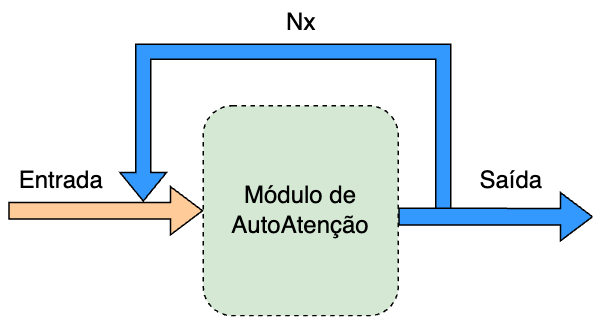
\includegraphics[width=0.7\textwidth]{figures/fig030.png}
    \caption*{Fonte: Autor}
    \label{fig:fig030}
\end{figure}


% Posso elencar novamente de forma sucinta os hiperparamentros aqui: EMBED_SIZE, N attention blocks, imagems de mascara e nova forma de concatenar. 


%--------------------------------------------------------
% \section{Cronograma}
% \label{sec:cronograma}

% O cronograma proposto das atividades segue na Figura \ref{fig:fig014}. Os itens em azul são atividades concluídas como: disciplinas, revisão bibliográfica, refinamento do tema, testes iniciais, etc. Itens em rosa são atividades em andamento como: implementação de modelos de comparação e escrita da dissertação. Atividades em amarelo são atividades planejadas como: análise de resultados, escrita da dissertação e escrita de artigos.

% \begin{figure}[htbp]
%     \centering
%     \caption{Cronograma planejado}
%     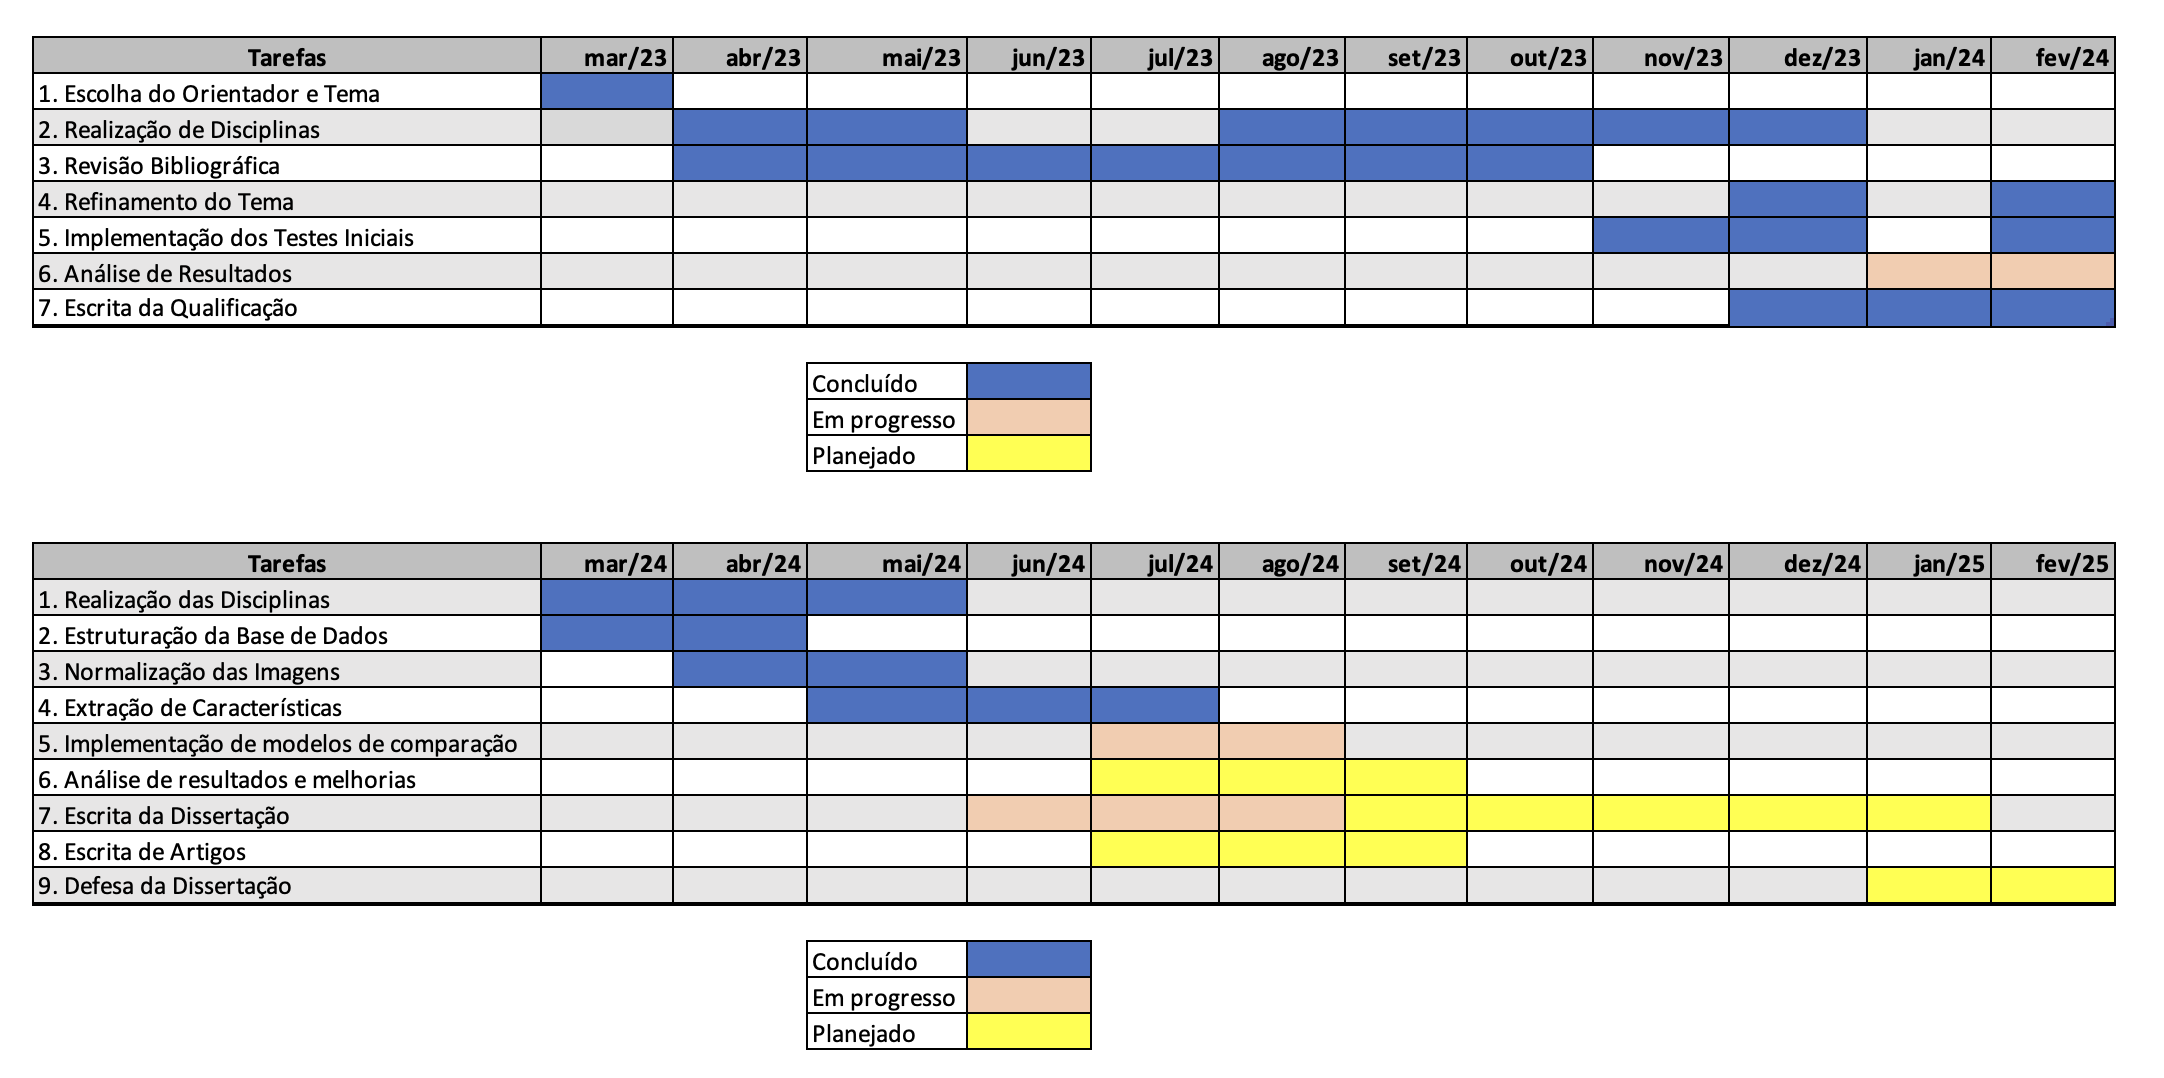
\includegraphics[width=1\textwidth]{figures/fig014.png}
%     \caption*{Fonte: Autor}
%     \label{fig:fig014}
% \end{figure}

%--------------------------------------------------------
\section{RESULTADOS ACDC}
\label{sec:resultados_acdc}

O conjunto de dados \gls{ACDC} foi a referência inicial, principalmente para a coleta dos resultados com o modelo base. Este conjunto de dados público já se encontra separado com $100$ exames para treino e $50$ para testes. A Figura \ref{fig:fig018} e \ref{fig:fig019} são exemplos respectivamente, de imagens de \gls{DCM} e \gls{HCM} capturadas na diástole com suas respectivas máscaras, lembrando que ambas representam cardiomiopatia hipertrófica. Na Figura \ref{fig:fig020} temos a imagem de coração em estado sem anomalia (\gls{NOR}) e sua respectiva máscara. As imagens demonstradas fazem parte do conjunto real de treinamento.

\begin{figure}[h!]
    \centering
    \caption{Captura Diastólica CMD}
    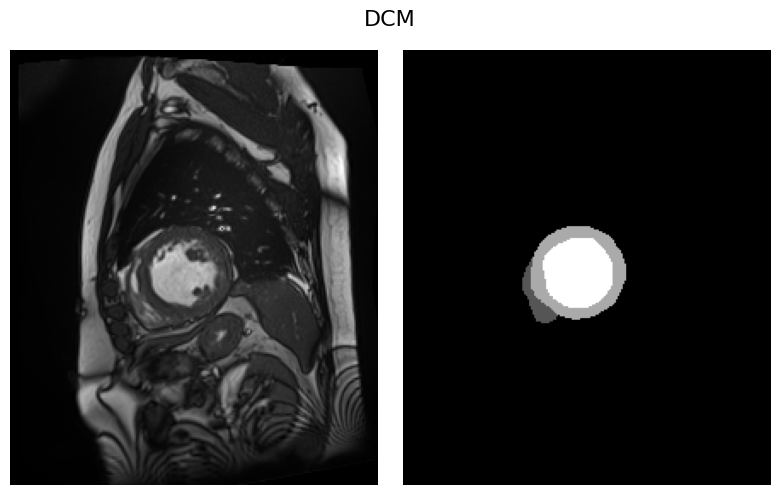
\includegraphics[width=0.65\textwidth]{figures/fig018.png}
    \caption*{Fonte: Autor}
    \label{fig:fig018}
\end{figure}

\begin{figure}[h!]
    \caption{Captura Diastólica de CMH}
    \centering
    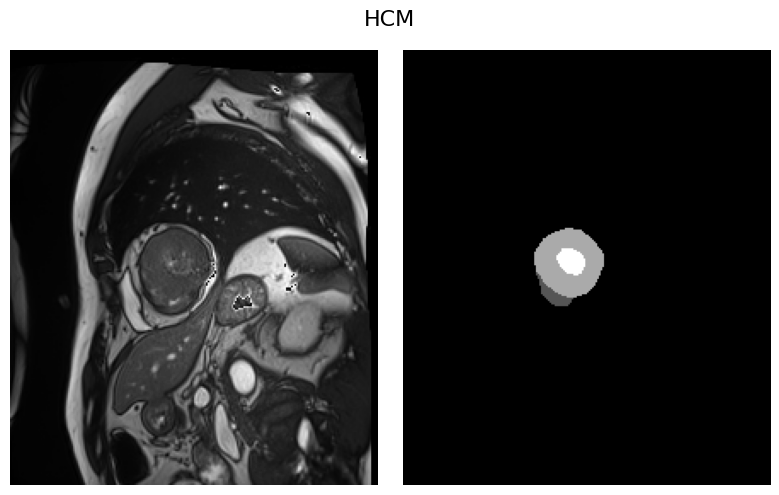
\includegraphics[width=0.65\textwidth]{figures/fig019.png}
    \caption*{Fonte: Autor}
    \label{fig:fig019}
\end{figure}

\begin{figure}[h!]
    \centering
    \caption{Captura Diastólica NOR}
    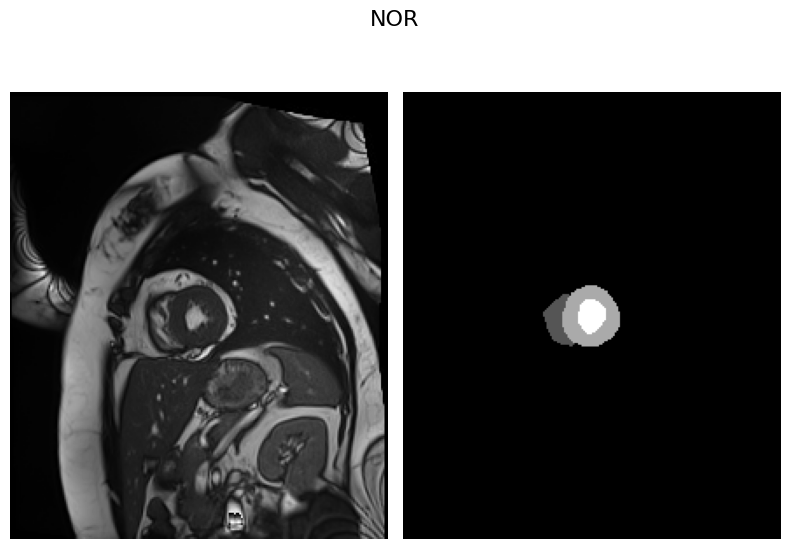
\includegraphics[width=0.65\textwidth]{figures/fig020.png}
    \caption*{Fonte: Autor}
    \label{fig:fig020}
\end{figure}

%--------------------------------------------------------
\subsection{Resultados dos Modelos Base - ACDC}
\label{subsec:resultados_acdc_base}

Com os dados pré-processados e previamente armazenados, o treinamento é efetuado com os vetores radiômicos e profundos. As métricas parciais foram sendo salvas em tempo de treinamento. Para o modelo base os hiperparâmetros são: $\text{EMBED}_{size}$ igual a $12$, $N$ igual 1, ou seja, apenas um bloco de auto atenção, dimensão de concatenação $1$, taxa de aprendizado $\LR$, otimizador \gls{Adam}, tamanho de lote $\Batch$ e aproximadamente $\Epochs$ épocas. Uma vez treinado, foi feita a inferência no conjunto de dados de teste, aplicando a função sigmoide e definindo $0,5$ como o valor de corte onde os valores acima deste limite são classificados como \gls{CAR} e os demais como sem cardiomiopatia. 

As métricas resultantes podem ser conferidas na Tabela \ref{tab:metrics}. A matriz de confusão é apresentada na Figura \ref{fig:fig016} e um gráfico ilustrando da \gls{ROC} é apresentado na Figura \ref{fig:fig017}.
\newline

\begin{table}[h!]
    \centering
    \caption{Métricas do Experimento - Modelo Base}
    \renewcommand{\arraystretch}{1} % default é 1 
    \begin{tabular}{|c|c|}
    \hline 
          \textbf{Métrica} & \textbf{Valor} \\ 
    \hline 
        Acurácia & 0.58 \\ 
    \hline 
        Precisão & 0.47 \\ 
    \hline 
        Revocação & 0.45 \\ 
    \hline 
        AUC & 0.55 \\ 
    \hline 
    \end{tabular} 
    \caption*{Fonte: Autor}
    \label{tab:metrics}
\end{table}

\begin{figure}[h!]
    \centering
    \caption{Matriz de Confusão -  Modelo Base}
    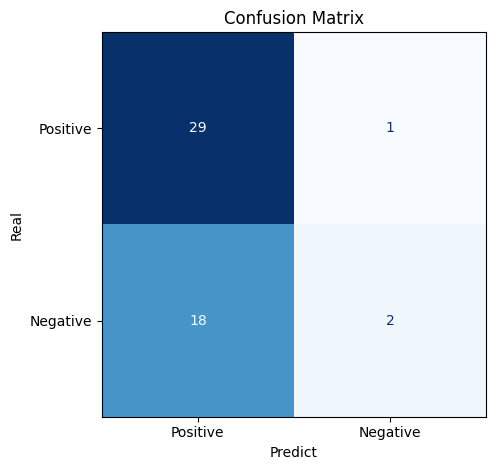
\includegraphics[width=0.55\textwidth]{figures/fig016.png}
    \caption*{Fonte: Autor}
    \label{fig:fig016}
\end{figure}

\begin{figure}[h!]
    \centering
    \caption{ROC}
    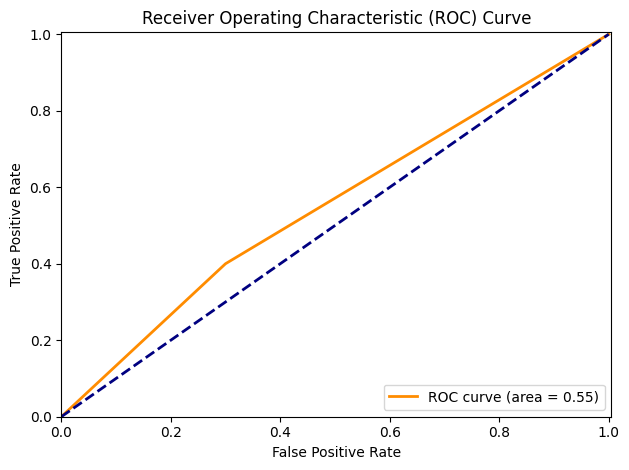
\includegraphics[width=0.75\textwidth]{figures/fig017.png}
    \caption*{Fonte: Autor}
    \label{fig:fig017}
\end{figure}


Para o registro dos resultados foi utilizado a ferramenta \textit{CometML}. O \textit{CometML} pode registrar, em tempo de execução, informações como erro por lote, erro por época, acurácia de validação, etc, podem ser armazenados enquanto o processo de treinamento é executado. Por fim métricas como acurácia e matriz de confusão podem ser armazenadas também. O serviço é acessado  por uma \gls{API} externa. As Figuras \ref{fig:fig028} e \ref{fig:fig029} demonstram respectivamente os painéis adaptáveis com alguns dos hiperparâmetros e métricas coletadas durante e ao terminar o treino. É possível notar que o modelo se sobre-ajusta nos dados de treino, com acurácia $1$, predizendo corretamente todos os valores porém, nos dados de teste a assertividade cai drasticamente para $0,58$. Também é possível notar que após $2500$ passos no treinamento, o erro de treinamento estabiliza e os demais processamentos não se fazem necessários.

\begin{figure}[h!]
    \centering
    \caption{Painéis Adaptáveis - \textit{CometML}}
    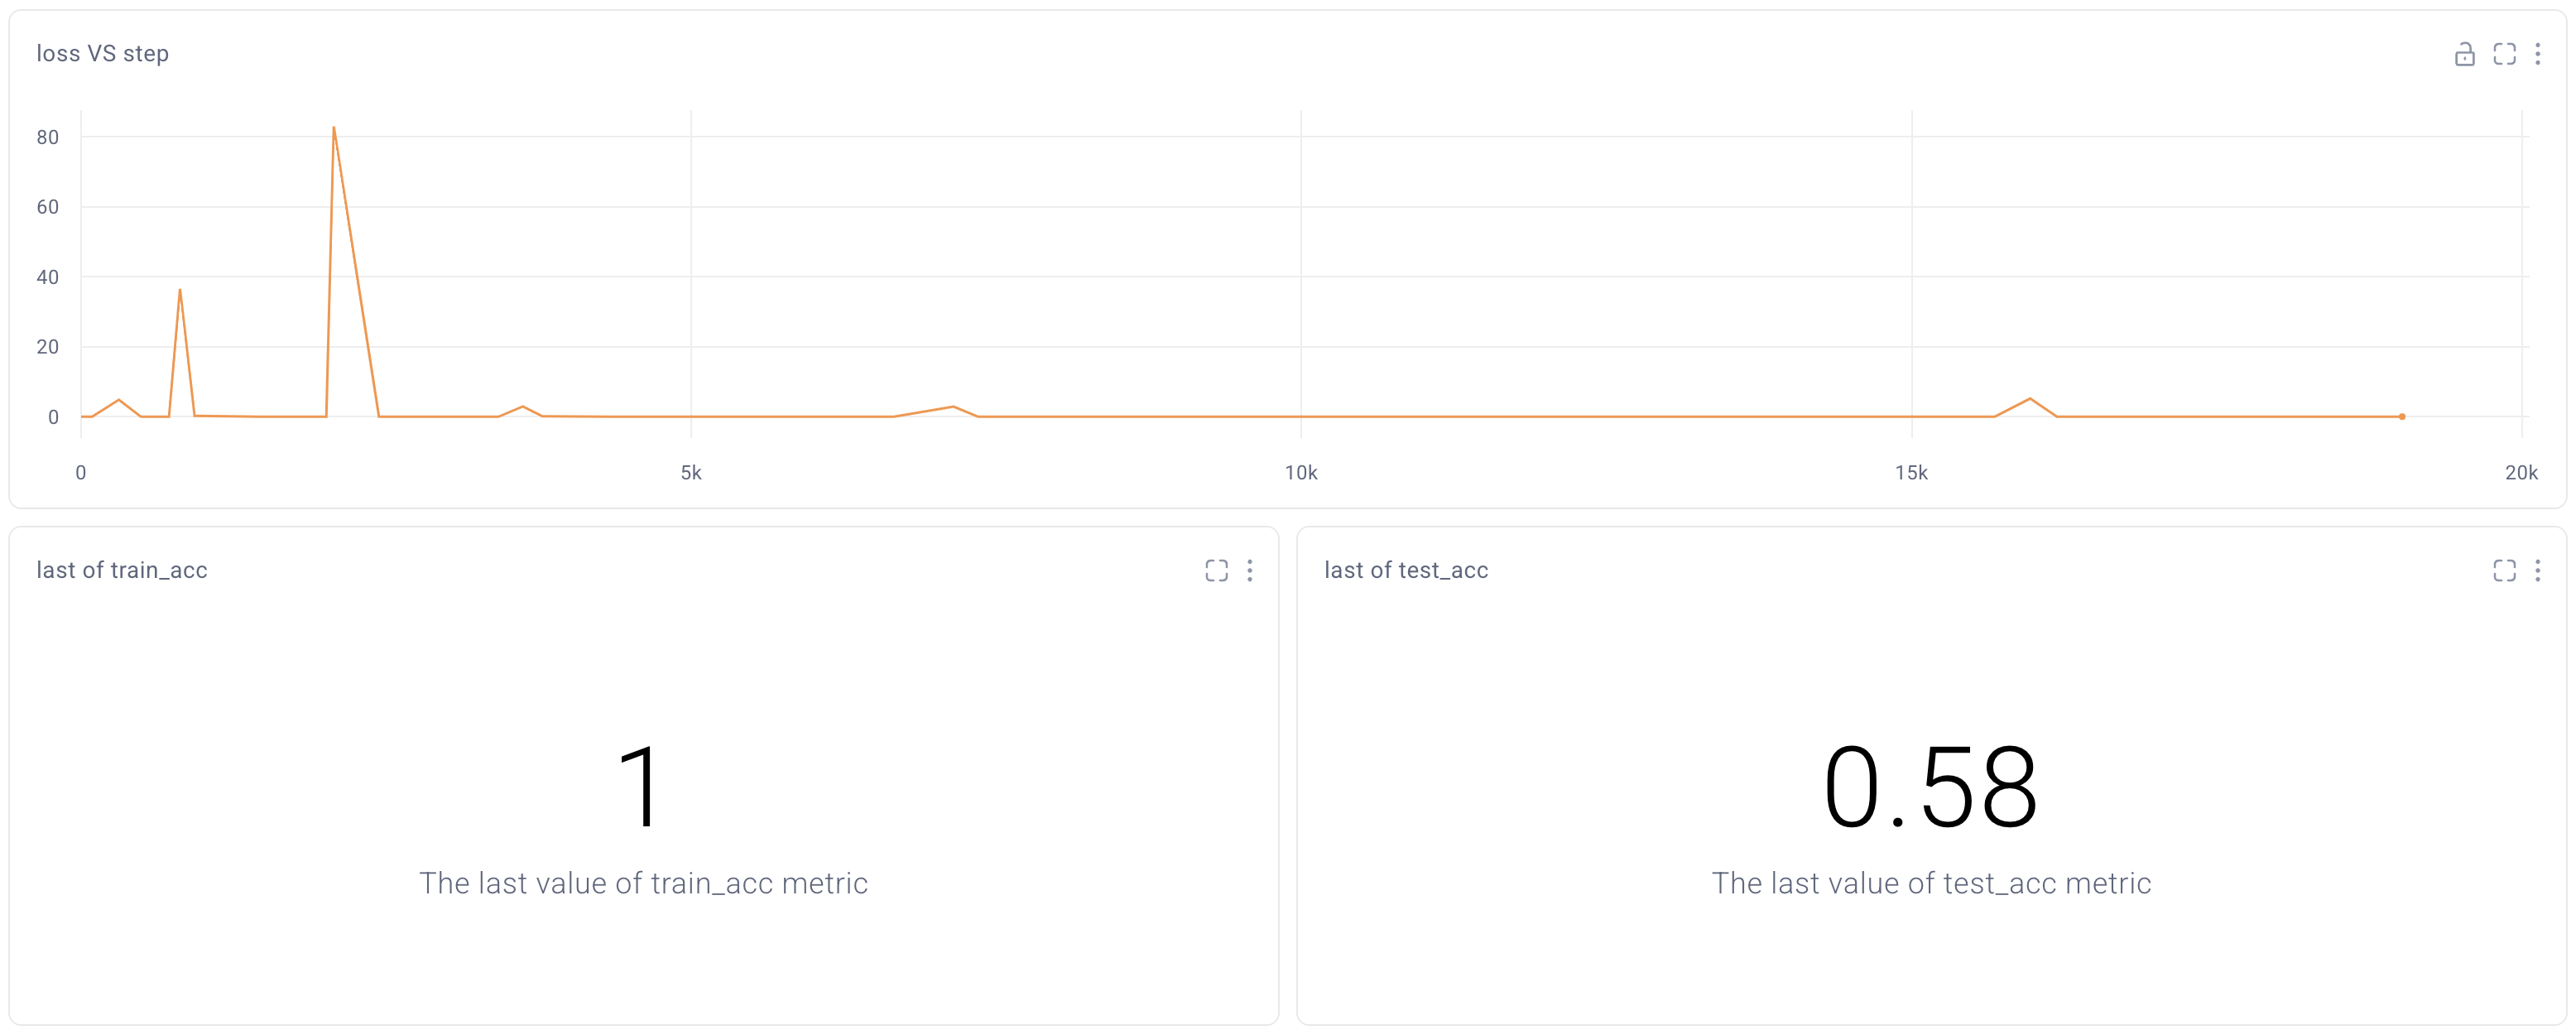
\includegraphics[width=1\textwidth]{figures/fig028.png}
    \caption*{Fonte: Autor}
    \label{fig:fig028}
\end{figure}


\begin{figure}[h!]
    \centering
    \caption{Valores Coletados no Treino - \textit{CometML}}
    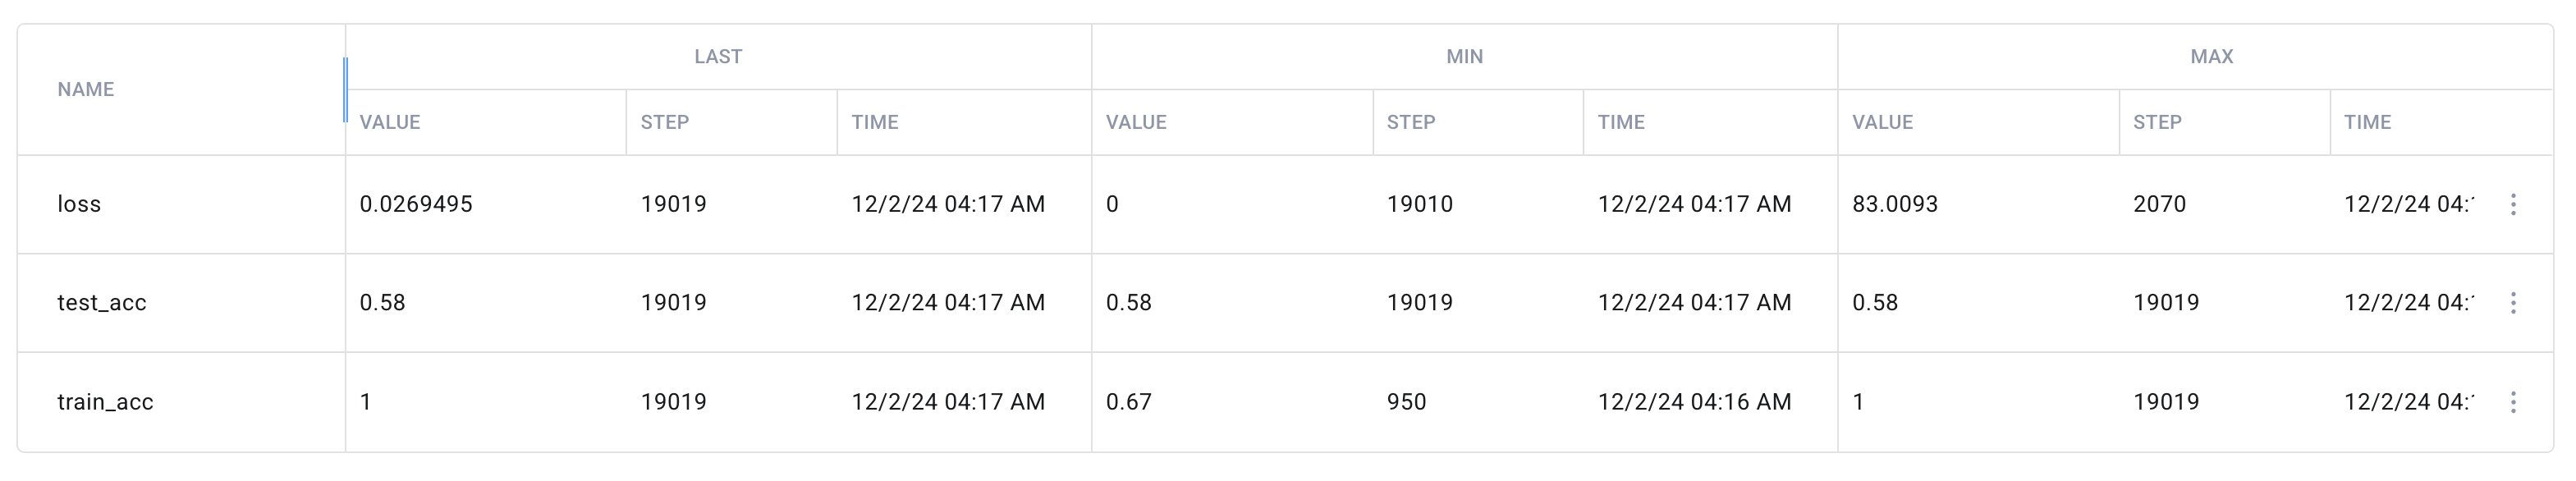
\includegraphics[width=1\textwidth]{figures/fig029.png}
    \caption*{Fonte: Autor}
    \label{fig:fig029}
\end{figure}


%--------------------------------------------------------
\subsection{Resultados dos Modelos Adaptados - ACDC}
\label{subsec:resultados_acdc_adaptado}

Para as versões adaptadas, se buscou mudar os hiperparâmetros e até mesmo a arquitetura do modelo com o intuito comparar os resultados com a versão base. Os primeiros experimentos foram aplicados variando o $\text{EMBED}_{size}$, também foi aplicado $N$ vezes o bloco de autoatenção ao invés de uma única vez. Os experimentos foram executado gerando a combinatória destes hiperparâmetros para cobrir o máximo de cenários possíveis dentro da metodologia.

Também foi introduzido, nas versões adaptadas, um módulo convolucional, que antecede o módulo de autoatenção. Este módulo convolucional é composto de três blocos: uma camada convolucional 1D, um bloco \gls{SE} e outro bloco convolucional 1D. Com a possibilidade de se ter adicionar opcionalmente um terceiro vetor de características, sendo este a máscara, foi possível identificar relações intrínsecas entre mais este vetor. A concatenação agora na primeira dimensão faz cada vetor de característica se tornar um canal. 

No módulo convolucional, uma primeira camada de convolução 1D aumenta o número de canais para $16$, ou seja, $16$ filtros são aplicado para extração de informação espacial. O bloco \gls{SE} representa a camada de atenção seletiva que dá importância aos canais mais importantes, identificando a relevância de cada canal e finaliza escalando os canais na entrada original com um valor escalar otimizado em tempo de treinamento. Detalhes podem ser vistos na Figura \ref{fig:fig031}. O bloco \gls{SE} neste projeto é adaptado para ser 1D, diferente do trabalho original que visa sua aplicação em modelos de visão computacional já consolidados. O valor de $r$ no bloco \gls{SE} ficou fixo em $16$, os autores do trabalho original fazem testes empíricos e confirmam que o valor de $16$ é que traz melhores resultados.

\begin{figure}[h!]
    \centering
    \caption{Composição Bloco SE}
    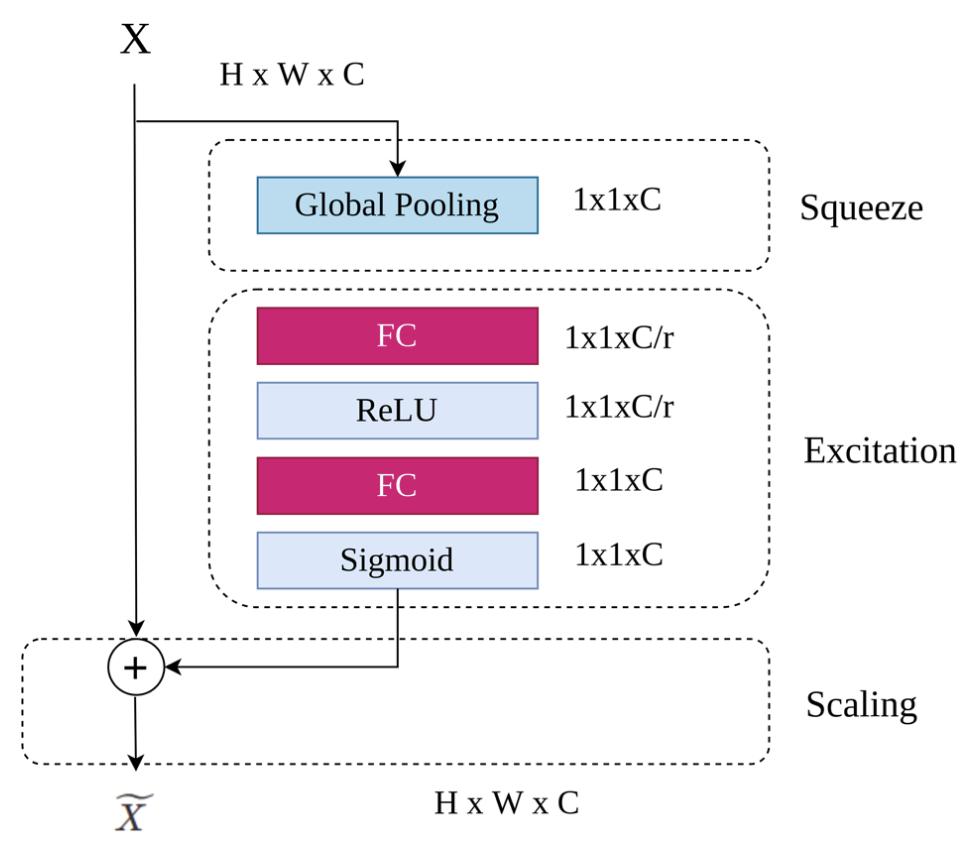
\includegraphics[width=0.7\textwidth]{figures/fig031.png}
    \caption*{Fonte: Adaptado de \cite{lafraxoSEDARUnetSqueezeexcitationDilated2024}}
    \label{fig:fig031}
\end{figure}


A Tabela \ref{tab:metrics_acdc_orig} apresenta o conjunto de experimentos na versão original e versões adaptadas. A Tabela \ref{tab:metrics_acdc_orig_mask} demonstra os experimentos adicionando a máscara como um terceiro vetor de características. A Tabela \ref{tab:metrics_acdc_se} apresenta a adição de blocos convolucionais e  \gls{SE}. Alguns pontos podem ser notados no experimento, o treinamento quase sempre sofre sobre-ajuste ficando muito próximo de 100\% de assertividade, isso pode se justificado dado o fato de haver poucos exemplares para treinamento. Outro ponto notado é que quanto maior o tamanho do vetor de características (Emb) melhor costuma ser o resultado. Quantidades maiores no número de blocos de autoatenção (N\_Attn) também melhoram os resultados, exceto no caso em que são configurados em $6$. A justificativa se deve ao fato de tornar o modelo mais complexos se comparados a quantidade de dados para treino, prejudicando a sua capacidade de generalização. Os melhores resultados são conferidos nas versões que adicionam o bloco \gls{SE} e com quatro blocos de autoatenção, sendo que o melhor experimento obteve $78\%$ de assertividade.


\begin{table}[htbp]
\centering
\caption{Métricas ACDC - Adaptação do Modelo Original
\newline Negrito representa o modelo base}
\begin{tabular}{lcccccc}
\toprule
\textbf{Emb} & \textbf{N\_Attn} & \textbf{Acc} & \textbf{Precision} & \textbf{Recall} & \textbf{F1} & \textbf{AUC} \\
\midrule
\textbf{24} & \textbf{1} & \textbf{0.58} & \textbf{0.47} & \textbf{0.45} & \textbf{0.46} & \textbf{0.55} \\
24 & 2 & 0.58 & 0.48 & 0.60 & 0.53 & 0.58 \\
24 & 4 & 0.54 & 0.44 & 0.55 & 0.49 & 0.54 \\
24 & 6 & 0.50 & 0.41 & 0.55 & 0.47 & 0.51 \\
\hline
48 & 1 & 0.62 & 0.52 & 0.55 & 0.54 & 0.61 \\
48 & 2 & 0.64 & 0.54 & 0.65 & 0.59 & 0.64 \\
48 & 4 & 0.66 & 0.56 & 0.70 & 0.62 & 0.67 \\
48 & 6 & 0.64 & 0.54 & 0.70 & 0.61 & 0.65 \\
\hline
64 & 1 & 0.62 & 0.52 & 0.65 & 0.58 & 0.62 \\
64 & 2 & 0.64 & 0.54 & 0.70 & 0.61 & 0.65 \\
64 & 4 & 0.66 & 0.57 & 0.65 & 0.60 & 0.66 \\
64 & 6 & 0.64 & 0.54 & 0.65 & 0.59 & 0.64 \\
\bottomrule
\end{tabular}
\caption*{Fonte: Autor}
\label{tab:metrics_acdc_orig}
\end{table}


\begin{table}[htbp]
\centering
\caption{Métricas ACDC - Adaptação do Modelo Original + Máscaras
\newline Negrito representa maior assertividade}
\begin{tabular}{lcccccc}
\toprule
\textbf{Emb} & \textbf{N\_Attn} & \textbf{Acc} & \textbf{Precision} & \textbf{Recall} & \textbf{F1} & \textbf{AUC} \\
\midrule
24 & 1 & 0.44 & 0.35 & 0.45 & 0.39 & 0.44 \\
24 & 2 & 0.46 & 0.38 & 0.55 & 0.45 & 0.48 \\
24 & 4 & 0.48 & 0.36 & 0.40 & 0.38 & 0.47 \\
24 & 6 & 0.48 & 0.38 & 0.45 & 0.41 & 0.47 \\
\hline
48 & 1 & 0.52 & 0.44 & 0.70 & 0.54 & 0.55 \\
48 & 2 & 0.58 & 0.48 & 0.55 & 0.51 & 0.57 \\
48 & 4 & 0.62 & 0.52 & 0.60 & 0.56 & 0.62 \\
48 & 6 & 0.60 & 0.50 & 0.50 & 0.50 & 0.58 \\
\hline
64 & 1 & 0.58 & 0.48 & 0.60 & 0.53 & 0.58 \\
64 & 2 & 0.56 & 0.45 & 0.50 & 0.48 & 0.55 \\
\textbf{64} & \textbf{4} & \textbf{0.64} & \textbf{0.54} & \textbf{0.65} & \textbf{0.59} & \textbf{0.64} \\
64 & 6 & 0.62 & 0.53 & 0.45 & 0.49 & 0.59 \\
\bottomrule
\end{tabular}
\caption*{Fonte: Autor}
\label{tab:metrics_acdc_orig_mask}
\end{table}


\begin{table}[htbp]
\centering
\caption{Métricas ACDC - Modelos Adaptados - Blocos Conv. + SE
\newline Negrito representa maior assertividade}
\begin{tabular}{lcccccc}
\toprule
\textbf{Emb} & \textbf{N\_Attn} & \textbf{Acc} & \textbf{Precision} & \textbf{Recall} & \textbf{F1} & \textbf{AUC} \\
\midrule
24 & 1 & 0.66 & 0.56 & 0.70 & 0.62 & 0.67 \\
24 & 2 & 0.68 & 0.58 & 0.75 & 0.65 & 0.69 \\
24 & 4 & 0.70 & 0.59 & 0.80 & 0.68 & 0.72 \\
24 & 6 & 0.68 & 0.59 & 0.65 & 0.62 & 0.67 \\
\hline
48 & 1 & 0.70 & 0.58 & 0.90 & 0.71 & 0.73 \\
48 & 2 & 0.70 & 0.62 & 0.65 & 0.63 & 0.69 \\
48 & 4 & 0.74 & 0.65 & 0.75 & 0.70 & 0.74 \\
48 & 6 & 0.70 & 0.60 & 0.75 & 0.67 & 0.71 \\
\hline
64 & 1 & 0.64 & 0.54 & 0.65 & 0.59 & 0.64 \\
64 & 2 & 0.72 & 0.64 & 0.70 & 0.67 & 0.72 \\
\textbf{64} & \textbf{4} & \textbf{0.78} & \textbf{0.76} & \textbf{0.65} & \textbf{0.70} & \textbf{0.76} \\
64 & 6 & 0.76 & 0.65 & 0.85 & 0.74 & 0.77 \\
\bottomrule
\end{tabular}
\caption*{Fonte: Autor}
\label{tab:metrics_acdc_se}
\end{table}


% \begin{figure}[h!]
%     \centering
%     \caption{Modelos c/ Bloco SE e sua Acurácia - \textit{CometML}}
%     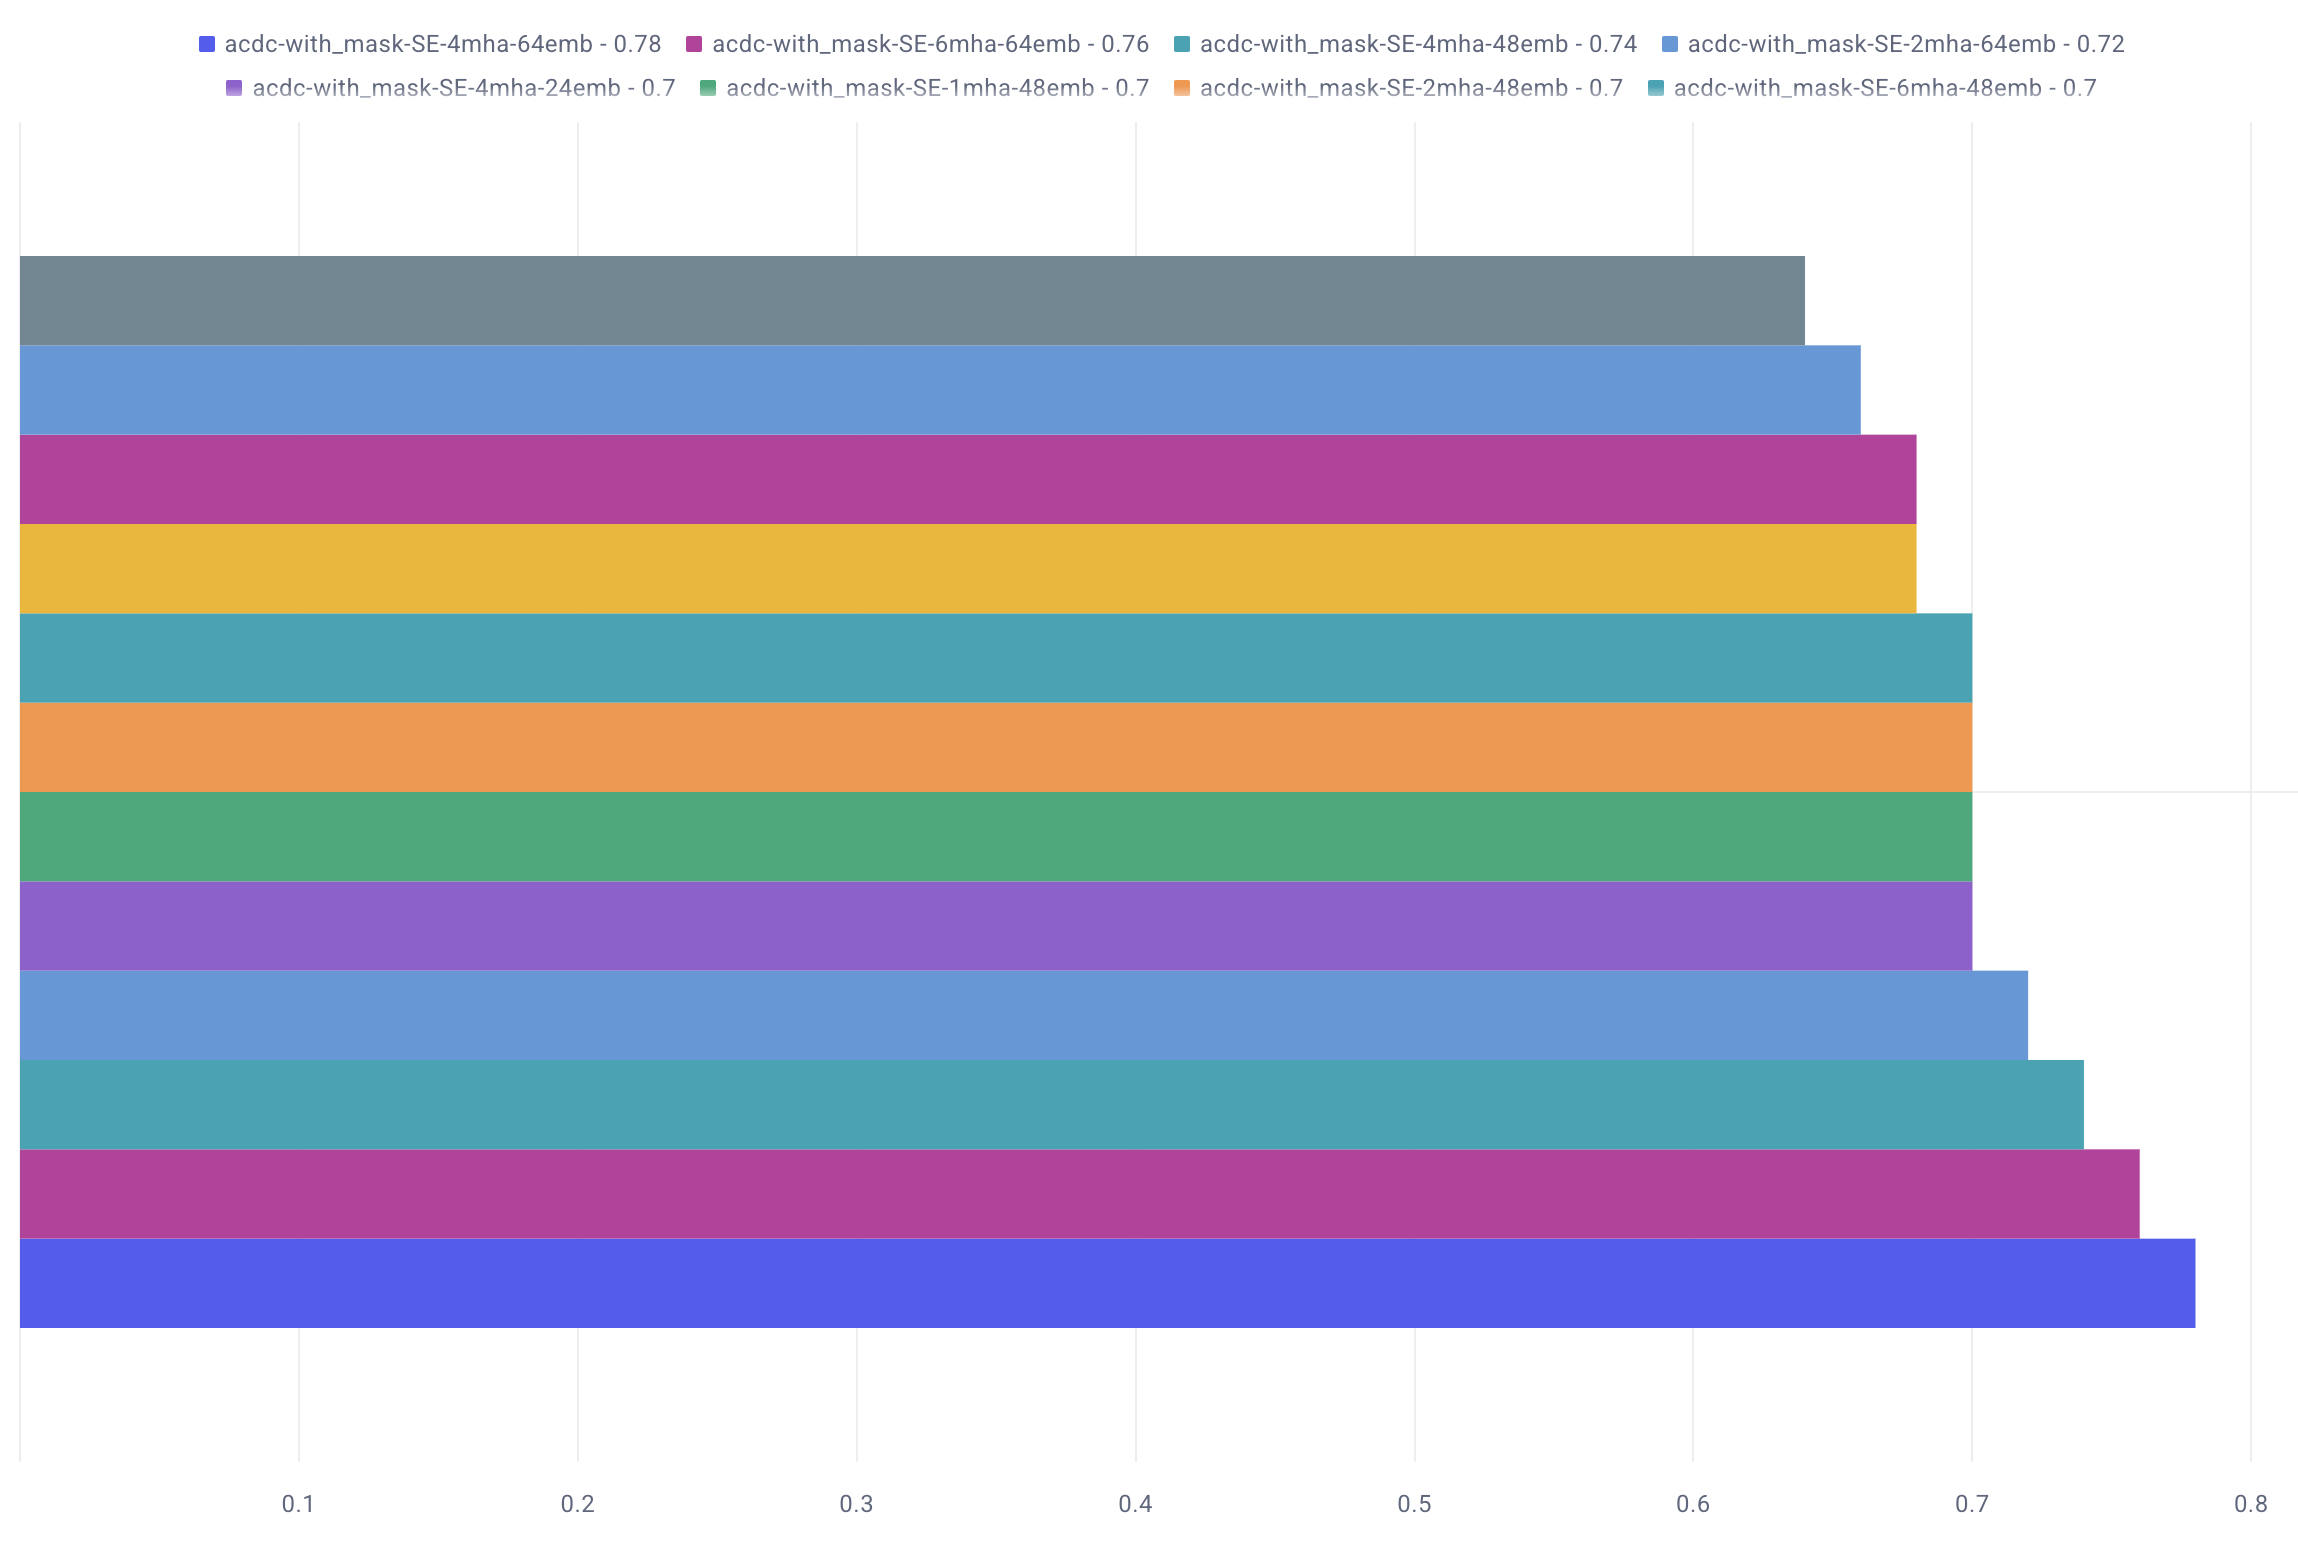
\includegraphics[width=1\textwidth]{figures/fig032.png}
%     \caption*{Fonte: Autor}
%     \label{fig:fig032}
% \end{figure}

%--------------------------------------------------------
\subsection{Resultados dos Modelos Adaptados - \textit{SunnyBrook}}
\label{subsec:resultados_sunny_adaptado}

Os experimentos no conjunto de dados \textit{SunnyBrook} foram os mesmos aplicados ao conjunto de dados \gls{ACDC}. No conjunto de dados \textit{SunnyBrook}, houve uma etapa extra de pré-processamento para gerar as máscaras. Foi necessário interpolar os valores de um arquivo de texto que vem anexo com os dados. A máscara também é composta apenas pela região de interesse com valores entre 0 e 1.

Como o \textit{SunnyBrook} tem poucos dados, apenas $45$, sendo $30$ para treino e $15$ para teste e removendo as classes de infarto (IC e IC-I), sobram $21$ registros sendo $13$ para treino e $8$ para teste. Foi considerado que o treinamento neste conjunto de dados não seria benéfico, pela quantidade limitada. Foi aplicado apenas as inferências considerando os $21$ registros, sendo $12$ casos de \gls{CMH} e $9$ casos em condições sem cardiomiopatia. Os modelos utilizados são os previamente treinados no \gls{ACDC}. Os resultados são conferidos nas tabelas \ref{tab:metrics_sunny_orig}, \ref{tab:metrics_sunny_orig_mask} e \ref{tab:metrics_sunny_se}. O modelo base consta em laranja e o melhor resultado consta em azul, indo de encontro aos resultados obtidos no \gls{ACDC}. É possível notar que o conjunto de dados, por ser pequeno, compromete a classificação pois mesmo que o modelo possua um pequeno aprimoramento de uma arquitetura para outra, pode não ser suficiente para converter uma nova classificação, o que da a aparência de que alguns modelos possuem a mesma capacidade, o que não é a realidade.


\begin{table}[htbp]
\centering
\caption{Métricas SunnyBrook - Adaptação do Modelo Original
\newline Negrito representa o modelo base}
\begin{tabular}{ccccccc}
\toprule
\textbf{Emb} & \textbf{N\_Attn} & \textbf{Acc} & \textbf{Precision} & \textbf{Recall} & \textbf{F1} & \textbf{AUC} \\
\midrule
\textbf{24} & \textbf{1} & \textbf{0.48} & \textbf{0.54} & \textbf{0.58} & \textbf{0.56} & \textbf{0.46} \\
24 & 2 & 0.52 & 0.60 & 0.50 & 0.55 & 0.53 \\
24 & 4 & 0.52 & 0.60 & 0.50 & 0.55 & 0.53 \\
24 & 6 & 0.52 & 0.57 & 0.67 & 0.62 & 0.50 \\
48 & 1 & 0.48 & 0.56 & 0.42 & 0.48 & 0.49 \\
48 & 2 & 0.48 & 0.55 & 0.50 & 0.52 & 0.47 \\
48 & 4 & 0.52 & 0.58 & 0.58 & 0.58 & 0.51 \\
48 & 6 & 0.52 & 0.60 & 0.50 & 0.55 & 0.53 \\
64 & 1 & 0.52 & 0.57 & 0.67 & 0.62 & 0.50 \\
64 & 2 & 0.57 & 0.64 & 0.58 & 0.61 & 0.57 \\
64 & 4 & 0.57 & 0.67 & 0.50 & 0.57 & 0.58 \\
64 & 6 & 0.52 & 0.57 & 0.67 & 0.62 & 0.50 \\
\bottomrule
\end{tabular}
\caption*{Fonte: Autor}
\label{tab:metrics_sunny_orig}
\end{table}


\begin{table}[htbp]
\centering
\caption{Métricas SunnyBrook - Adaptação do Modelo Original Com Máscaras
\newline Negrito representa maior assertividade}
\begin{tabular}{ccccccc}
\toprule
\textbf{Emb} & \textbf{N\_Attn} & \textbf{Acc} & \textbf{Precision} & \textbf{Recall} & \textbf{F1} & \textbf{AUC} \\
\midrule
24 & 1 & 0.48 & 0.54 & 0.58 & 0.56 & 0.46 \\
24 & 2 & 0.52 & 0.62 & 0.42 & 0.50 & 0.54 \\
24 & 4 & 0.57 & 0.67 & 0.50 & 0.57 & 0.58 \\
24 & 6 & 0.52 & 0.58 & 0.58 & 0.58 & 0.51 \\
48 & 1 & 0.52 & 0.58 & 0.58 & 0.58 & 0.51 \\
48 & 2 & 0.57 & 0.64 & 0.58 & 0.61 & 0.57 \\
48 & 4 & 0.62 & 0.67 & 0.67 & 0.67 & 0.61 \\
48 & 6 & 0.52 & 0.58 & 0.58 & 0.58 & 0.51 \\
64 & 1 & 0.57 & 0.62 & 0.67 & 0.64 & 0.56 \\
64 & 2 & 0.62 & 0.67 & 0.67 & 0.67 & 0.61 \\
\textbf{64} & \textbf{4} & \textbf{0.71} & \textbf{0.80} & \textbf{0.67} & \textbf{0.73} & \textbf{0.72} \\
64 & 6 & 0.62 & 0.64 & 0.75 & 0.69 & 0.60 \\
\bottomrule
\end{tabular}
\caption*{Fonte: Autor}
\label{tab:metrics_sunny_orig_mask}
\end{table}


\begin{table}[htbp]
\centering
\caption{Métricas SunnyBrook - Adaptação Adicionando Blocos Conv. e SE
\newline Negrito representa maior assertividade}
\begin{tabular}{ccccccc}
\toprule
\textbf{Emb} & \textbf{N\_Attn} & \textbf{Acc} & \textbf{Precision} & \textbf{Recall} & \textbf{F1} & \textbf{AUC} \\
\midrule
24 & 1 & 0.67 & 0.73 & 0.67 & 0.70 & 0.67 \\
24 & 2 & 0.71 & 0.80 & 0.67 & 0.73 & 0.72 \\
24 & 4 & 0.76 & 0.77 & 0.83 & 0.80 & 0.75 \\
24 & 6 & 0.71 & 0.75 & 0.75 & 0.75 & 0.71 \\
48 & 1 & 0.71 & 0.80 & 0.67 & 0.73 & 0.72 \\
48 & 2 & 0.76 & 0.82 & 0.75 & 0.78 & 0.76 \\
48 & 4 & 0.76 & 0.73 & 0.92 & 0.81 & 0.74 \\
48 & 6 & 0.76 & 0.89 & 0.67 & 0.76 & 0.78 \\
64 & 1 & 0.76 & 0.82 & 0.75 & 0.78 & 0.76 \\
64 & 2 & 0.81 & 0.90 & 0.75 & 0.82 & 0.82 \\
\textbf{64} & \textbf{4} & \textbf{0.86} & \textbf{0.85} & \textbf{0.92} & \textbf{0.88} & \textbf{0.85} \\
64 & 6 & 0.81 & 0.90 & 0.75 & 0.82 & 0.82 \\
\bottomrule
\end{tabular}
\caption*{Fonte: Autor}
\label{tab:metrics_sunny_se}
\end{table}

%--------------------------------------------------------
\section{CONSIDERAÇÕES FINAIS DO CAPÍTULO} 
\label{sec:cap6_consideracoes_finais}

Os resultados obtidos, aplicando a arquitetura original proposta por \citeonline{aiSelfAttentionBasedFusion2023} e a aplicação de diversas modificações, como a forma de concatenar para propiciar um módulo convolucional de extrair informações inter-relacionadas entre características extraídas de diferentes técnicas, a adição de um mecanismo de atenção seletiva na forma de um bloco \gls{SE} antecedente ao mecanismo de autoatenção, seguiram um padrão de resultados esperados. Conforme o modelo aumenta, seus resultados também melhoram mas com ganhos mínimos dependendo do caso. Adicionar técnicas relevantes como o bloco \gls{SE} aprimorou os resultados significativamente.

A atenção seletiva procura gera um conjunto de pesos ao ao prever diretamente a importância de cada parte dos dados, aprendendo o valor dos pesos para cada canal no mapa de características com o objetivo de realçar ou suprimir as características de cada canal. O mecanismo de autoatenção envolve a utilização da correlação entre os conteúdos das camadas ocultas para calcular os pesos de atenção, que são então aplicados para agregar informações das camadas ocultas em uma escala global. Seguindo a intuição de utilizar diferentes mecanismos de atenção, conforme proposto pelos autores \cite{yangNeuralNetworkDesign2024a}, trouxe melhoras significativas comparadas ao modelo base. 

Outras adaptações também surtiram efeito, como aumentar o tamanho das características utilizadas, aplicar mais blocos de autoatenção, a adição das máscaras, etc. Os experimentos indicam que há espaço para exploração e melhorias, como por exemplo, outros mecanismos de atenção, podem trazer resultados ainda mais promissores para o âmbito de cardiomiopatia hipertrófica. 


\chapter{Resultados  Preliminares}
\label{chap:resultados_discussao}

%--------------------------------------------------------
\section{Resultados} 
\label{sec:cap6_resultados}

Os testes iniciais foram aplicados ao conjunto de dados do \gls{ACDC}. Este conjunto de dados público já vem separado com 100 exames para treino e 50 para testes. A Figura \ref{fig:fig018} e \ref{fig:fig019} são exemplos de imagens de \gls{DCM} e \gls{HCM} capturadas na diástole, ambas com suas máscaras. Na Figura \ref{fig:fig020} temos uma imagem de coração em estado normal (\gls{NOR}).

\begin{figure}[htbp]
    \caption{Captura Diastólica DCM}
    \centering
    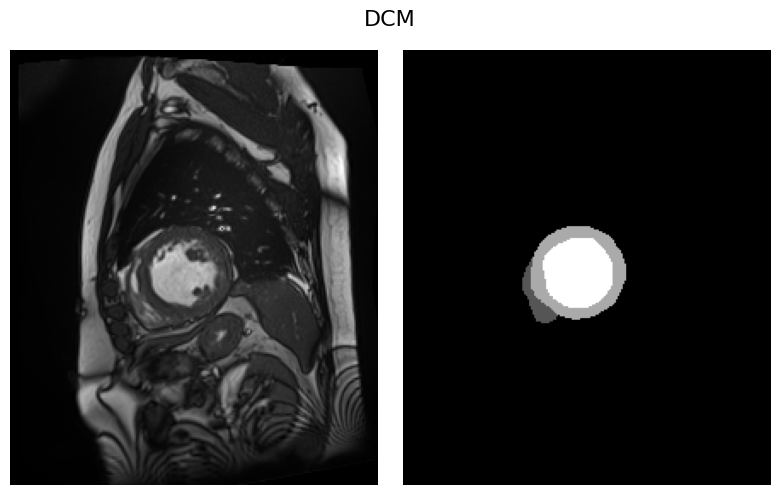
\includegraphics[width=0.65\textwidth]{figures/fig018.png}
    \caption{Fonte: Autor}
    \label{fig:fig018}
\end{figure}

\begin{figure}[htbp]
    \caption{Captura Diastólica de HCM}
    \centering
    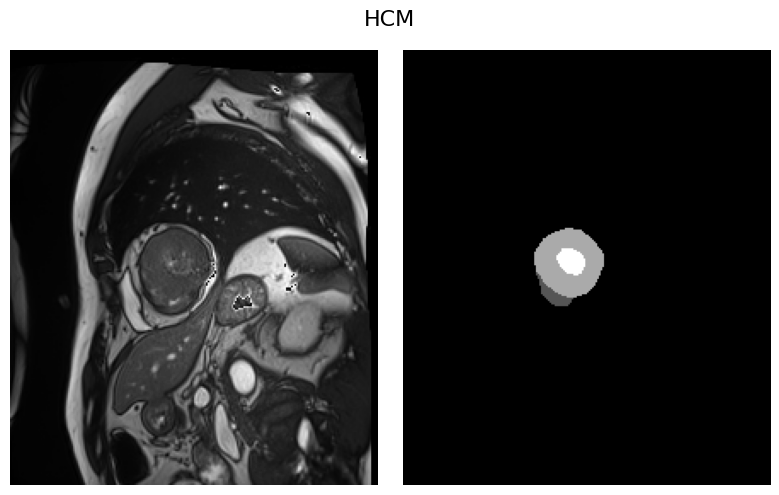
\includegraphics[width=0.65\textwidth]{figures/fig019.png}
    \caption{Fonte: Autor}
    \label{fig:fig019}
\end{figure}

\begin{figure}[htbp]
    \caption{Captura Diastólica NOR}
    \centering
    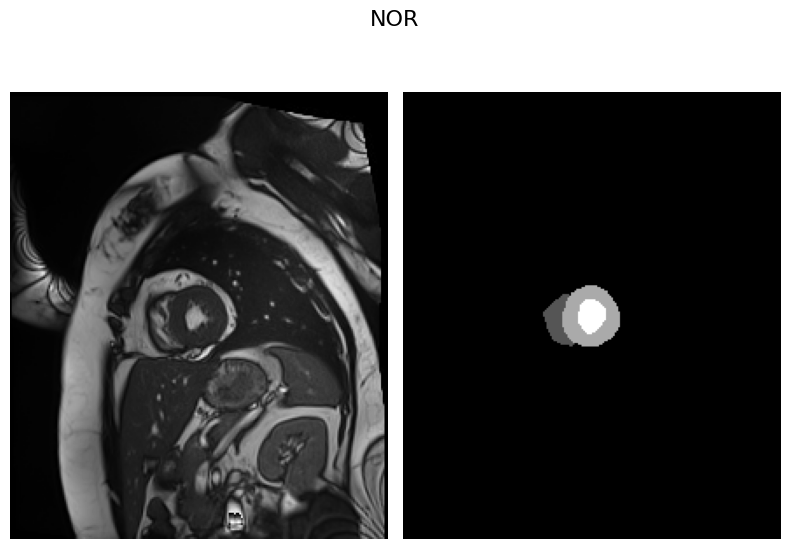
\includegraphics[width=0.65\textwidth]{figures/fig020.png}
    \caption{Fonte: Autor}
    \label{fig:fig020}
\end{figure}

Os resultados foram obtidos aplicando a metodologia previamente apresentada, foi extraídas as \textit{features} radiômicas e profundas, após foi aplicado o F-Test para seleção de \textit{features} e o resultado concatenado. Por fim, o modelo de \textit{self-attention} foi aplicado, os hiperparâmetros utilizados são: taxa de aprendizado $0,0001$, otimizador \gls{Adam} e aproximadamente 300 épocas. As principais métricas calculadas são conferidas na Tabela \ref{tab:metrics}.

\begin{table}[hbtp]
    \centering
    \renewcommand{\arraystretch}{1} % default é 1 
    \begin{tabular}{|c|c|}
    \hline 
          \textbf{Métrica} & \textbf{Valor} \\ 
    \hline 
        Acurácia & 0.62 \\ 
    \hline 
        Precisão & 0.67 \\ 
    \hline 
        Revocação & 0.10 \\ 
    \hline 
        AUC & 0.63 \\ 
    \hline 
    \end{tabular} 
    \caption{Fonte: Autor}
    \label{tab:metrics}
\end{table}

A matriz de confusão é conferida Figura \ref{fig:fig016}.

\begin{figure}[htbp]
    \caption{Matriz de Confusão}
    \centering
    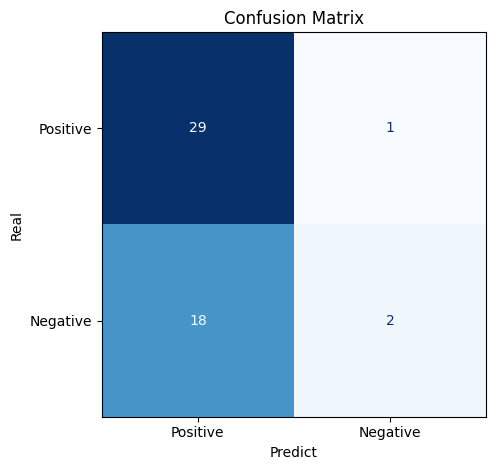
\includegraphics[width=0.55\textwidth]{figures/fig016.png}
    \caption{Fonte: Autor}
    \label{fig:fig016}
\end{figure}

Um gráfico ilustrativo da \gls{ROC} é visto na Figura \ref{fig:fig017}

\begin{figure}[htbp]
    \caption{ROC}
    \centering
    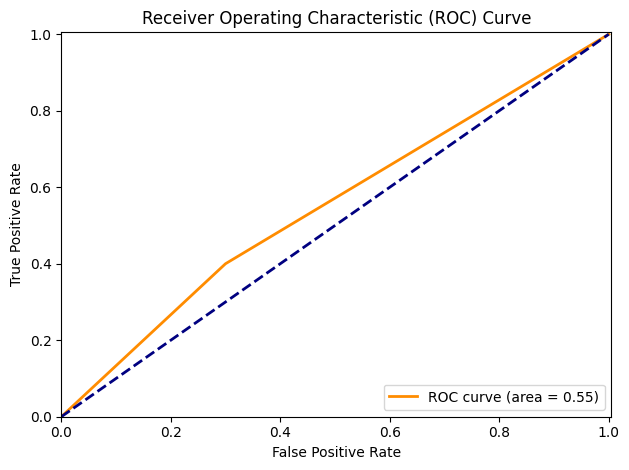
\includegraphics[width=0.75\textwidth]{figures/fig017.png}
    \caption{Fonte: Autor}
    \label{fig:fig017}
\end{figure}

%--------------------------------------------------------
\section{Conclusão dos Resultados} 
\label{sec:cap6_conclusãp_resultados}

Os resultados obtidos, diferente do trabalho similar aplicado à identificação de câncer no pulmão, obteve resultados pouco relevantes o que indica que há espaço para exploração e melhoria para o âmbito de \gls{CH}. Algumas, abordagens ainda são tidas em vista como manipular o seletor de \textit{features} e a sua quantidade, testar novos hiperparâmetros para os modelos, ao invés de ter um único módulo de \textit{self-attention}, aplicar vários em cascata, etc.


% %--------------------------------------------------------
% \subsection{Experimentos ACDC}
% \label{subsec:cap5_experimentos_acdc}




\chapter{CONCLUSÃO}
\label{chap:cap7_conclusao}

Este trabalho apresentou uma abordagem inovadora para a classificação de cardiomiopatias utilizando imagens de ressonância magnética cardiovascular (RMC) combinadas com mecanismos de atenção, promovendo a integração entre características radiômicas e profundas. A proposta foi construída com base em fundamentos teóricos sólidos, utilizando técnicas modernas de aprendizado profundo, como a arquitetura \gls{SE} Net e mecanismos de autoatenção, para explorar características discriminantes presentes em imagens médicas.

Os resultados obtidos destacaram a eficiência do modelo proposto na identificação de padrões associados a cardiomiopatias, superando abordagens tradicionais em termos de acurácia e generalização. A fusão de informações radiômicas, que capturam detalhes texturais e estatísticos, com características profundas extraídas de redes convolucionais, mostrou-se eficaz para lidar com a complexidade intrínseca das cardiomiopatias hipertróficas (CMH) e dilatadas (CMD). Além disso, o uso de mecanismos de atenção também permitiu priorizar as regiões mais relevantes das imagens, promovendo maior expressividade do modelo.

A utilização do mecanismo SE-ResNet e da atenção espacial no domínio de imagens médicas representou uma abordagem inovadora ao priorizar informações relevantes no mapa de características. Essa técnica não apenas melhorou o desempenho do modelo, mas também ofereceu uma forma mais intuitiva de explicar as decisões tomadas pela IA, um aspecto crucial para sua aceitação na prática clínica.

Embora os resultados sejam promissores, este trabalho também expôs limitações, como a necessidade de bases de dados mais robustas e diversificadas, além da dificuldade em interpretar os modelos de aprendizado profundo, um desafio recorrente na área médica. Contudo, o modelo proposto representa um avanço significativo na aplicação de inteligência artificial em diagnósticos médicos, contribuindo para o desenvolvimento de ferramentas mais precisas e acessíveis para o suporte à decisão clínica, especialmente no diagnóstico precoce e acompanhamento de cardiomiopatias. Essas ferramentas podem melhorar a eficiência dos profissionais de saúde, reduzindo o tempo de análise manual e permitindo intervenções mais rápidas e precisas.

O desenvolvimento e avaliação do modelo proposto trazem contribuições relevantes para a literatura de aprendizado profundo aplicado à medicina, ao demonstrar como características radiômicas e mecanismos de atenção podem ser combinados de forma eficaz. 

Por fim, os achados desta pesquisa abrem caminhos para futuras investigações, como a aplicação de mecanismos de atenção em outras doenças cardíacas e a integração de dados multimodais, incluindo genômicos e clínicos, para uma abordagem ainda mais abrangente e personalizada na medicina. O uso de técnicas avançadas, como aquelas desenvolvidas neste estudo, reforça o papel da inteligência artificial como uma aliada indispensável na medicina de precisão.

Como trabalhos futuros, sugere-se explorar a combinação de imagens médicas com dados clínicos e genéticos para criar modelos multimodais, que possam fornecer diagnósticos mais holísticos e personalizados. Além disso, o uso de técnicas como aprendizado federado pode ser investigado para proteger a privacidade dos dados enquanto se colabora em larga escala entre instituições.

%--------------------------------------------------------
\section{PUBLICAÇÕES GERADAS} 
\label{sec:cap7_publicacoes}

\lipsum[1-1]

\printbibliography
%\printindex

%\begin{anexo}

\appendix \centering \textbf{ANEXO 1} 


%\includepdf[pages=1-12]{documentos/ane1}

\appendix \centering \textbf{ANEXO 2}
%\includepdf [pages=1-7]{documentos/ane2}


%\end{anexo}




\end{document}
